%\documentclass[a4paper,UKenglish,cleveref, autoref, thm-restate]{lipics-v2019}
\documentclass[a4paper,anonymous,USenglish]{lipics-v2019}
\pdfminorversion=7 

\usepackage{amssymb}
\usepackage{color}
\usepackage{ifthen}
\usepackage{algorithm}
\usepackage{algpseudocode}
\usepackage{amsmath,multicol}
\usepackage{ioa_code}
\usepackage{graphicx}
\usepackage{subcaption}
\usepackage{diagbox}
\usepackage{enumitem}
\usepackage{booktabs}
\usepackage{subcaption}
\usepackage{cleveref}

  

%%%%%%%%%%%%%%%%%%%%%%%%%%%%%%%%%%%%%%%%%%%%%%
%%%%%% FORMATTING 
%%%%%%%%%%%%%%%%%%%%%%%%%%%%%%%%%%%%%%%%%%%%%%
\newcommand{\case}[1]{
        {\vspace{1em}\noindent{\bf Case #1:}}}
\newcommand{\subcase}[1]
	{{\emph{Case #1:}}}

%Efficiency Metric
\newcommand{\efficiency}{operation latency}

%floor
\newcommand{\floor}[1]{\left\lfloor #1 \right\rfloor}
%ceiling
\newcommand{\ceil}[1]{\lceil #1 \rceil}


%%%%%%%%%%%%%%%%%%%%%%%%%%%%%%%%%%%%%%%%%%%%%%
%%%%%% LIST OF SYMBOLS
%%%%%%%%%%%%%%%%%%%%%%%%%%%%%%%%%%%%%%%%%%%%%%

% Define List of Symbols
% Added by Nicolas Nicolaou
\makeatletter
\def\mainlistofsymbols{
  %\newpage
  %\vspace{.25in}
  %\begin{center}
  %  {\Large\bf LIST OF SYMBOLS}
  %\end{center}
  \normalsize
  \vspace*{1.5 em}
  \@starttoc{los}
}

\def\partonelistofsymbols{
  \normalsize
  \vspace*{1.5 em}
  \@starttoc{p1los}
}

\def\parttwolistofsymbols{
  \normalsize
  \vspace*{1.5 em}
  \@starttoc{p2los}
}

%% Define the formatting of the symbol entry in the addcontentsline command : NN
\def\l@symbol#1#2{\addpenalty{-\@highpenalty} \vskip 4pt plus 2pt
{\@dottedtocline{0}{0em}{8em}{#1}{#2}}}
\makeatother

% Command for list of symbols
%% The symbol appears in both the los and in place in the text : NN
\newcommand{\mainsym}[2]{%
#1%
\addcontentsline{los}{symbol}{\protect\numberline{#1}{#2}}
%\addtocontents{los}{\contentsline{symbol}{\protect\numberline{#1}{#2}}{}}
}

%% The symbol appears in both the los and in place in the text : NN
\newcommand{\partonesym}[2]{%
#1%
\addcontentsline{p1los}{symbol}{\protect\numberline{#1}{#2}}
}

%% The symbol appears in both the los and in place in the text : NN
\newcommand{\parttwosym}[2]{%
#1%
\addcontentsline{p2los}{symbol}{\protect\numberline{#1}{#2}}
}

%% The symbol does not appear in the text but only in the los : NN
\newcommand{\newhiddensym}[2]{%
%% NN uncomment next line to work
%\addcontentsline{los}{symbol}{\protect\numberline{#1}{#2}}
}




%%%%%%%%%%%%%%%%%%%%%%%%%%%%%%%%%%%%%%%%%%%%%%
%IOA
%%%%%%%%%%%%%%%%%%%%%%%%%%%%%%%%%%%%%%%%%%%%%%
\newcommand{\stateSet}[1]{states(#1)}
\newcommand{\startSet}[1]{start(#1)}
\newcommand{\actionSet}[1]{actions(#1)}
\newcommand{\inputSet}[1]{in(#1)}
\newcommand{\outputSet}[1]{out(#1)}
\newcommand{\internalSet}[1]{int(#1)}
\newcommand{\sigSet}[1]{sig(#1)}
\newcommand{\extsigSet}[1]{extsig(#1)}
\newcommand{\transSet}[1]{trans(#1)}
% Automata
\newcommand{\IOA}{A}
\newcommand{\algIOA}[2]{\ifmmode{\text{#1}_{#2}}\else{$\text{#1}_{#2}$}\fi}
% IOA assigned to process #1
\newcommand{\prIOA}[1]{A_{#1}}
\newcommand{\chIOA}[1]{\text{\sc Channel}_{#1}}
\newcommand{\rdIOA}[2]{\algIOA{#1}{#2}}
\newcommand{\wrtIOA}[2]{\algIOA{#1}{#2}}
\newcommand{\srvIOA}[2]{\algIOA{#1}{#2}}
% Memory Automaton
\newcommand{\memIOA}{\mathcal{M}}
% Algorithm Automata
\newcommand{\abdIOA}[1]{\algIOA{\ABD}{#1}}
\newcommand{\fastIOA}[1]{\algIOA{\fast}{#1}}
\newcommand{\sliqIOA}[1]{\algIOA{\SLIQ}{#1}}
\newcommand{\cwfrIOA}[1]{\algIOA{\cwfr}{#1}}
\newcommand{\sfwIOA}[1]{\algIOA{\sfw}{#1}}

%%%%%%%%%%%%%%%%%%%%%%%%%%%%%%%%%%%%%%%%%%%%%%
% Executions and execution fragments
%%%%%%%%%%%%%%%%%%%%%%%%%%%%%%%%%%%%%%%%%%%%%%
\newcommand{\EX}{\ifmmode{\xi}\else{$\xi$}\fi}
\newcommand{\EXF}{\ifmmode{\phi}\else{$\phi$}\fi}
%Extend
\newcommand{\extend}[2]{#1\circ#2}
%Extracted execution
\newcommand{\extract}[2]{#1|#2}
%Actions
\newcommand{\acts}{\alpha}
%Execution Set
\newcommand{\execSet}[1]{execs(#1)}
%Good Executions Set for a particular failure pattern
\newcommand{\gexecSet}[2]{goodexecs(#1,#2)}
%General Good Executions Set
\newcommand{\ggexecSet}[1]{goodexecs(#1)}
%Event History
\newcommand{\hist}[1]{H_{#1}}
%Event History Fragment
\newcommand{\histf}[1]{H_{#1}}

%%%%%%%%%%%%%%%%%%%%%%%%%%%%%%%%%%%%%%%%%%%%%%
% States and State Variables
%%%%%%%%%%%%%%%%%%%%%%%%%%%%%%%%%%%%%%%%%%%%%%
%State of an automaton
\newcommand{\stt}{\sigma}
% Invocation Step
\newcommand{\invStep}[1]{inv(#1)}
\newcommand{\stInv}[1]{\stt_{\invStep{#1}}}
% Response Step
\newcommand{\resStep}[1]{res(#1)}
\newcommand{\stRes}[1]{\stt_{\resStep{#1}}}
%The value of variable #2 in state #1 of process #2 
\newcommand{\stVar}[3]{#1[#2].#3}
%Fix events (read, write, inform)
\newcommand{\stfix}[1]{\st_{fix(#1)}}

%%%%%%%%%%%%%%%%%%%%%%%%%%%%%%%%%%%%%%%%%%%%%%
% Object Type Notation
%%%%%%%%%%%%%%%%%%%%%%%%%%%%%%%%%%%%%%%%%%%%%%
%Object Response Set
\newcommand{\objResSet}[1]{\Gamma_{#1}}
%Object Operation Set
\newcommand{\objOpSet}[1]{\opSet_{#1}}
%Object State Set
\newcommand{\objStSet}[1]{\Sigma_{#1}}
%Object Transition Set
\newcommand{\objTSet}[1]{\Delta_{#1}}
%Object
\newcommand{\obj}[1]{O_{#1}}

%%%%%%%%%%%%%%%%%%%%%%%%%%%%%%%%%%%%%%%%%%%%%%
% Quorum systems
%%%%%%%%%%%%%%%%%%%%%%%%%%%%%%%%%%%%%%%%%%%%%%
\newcommand{\qs}{\mathbb{Q}}
% Biquorum System
\newcommand{\bs}{\mathbb{B}}
% Sub-Quorum system 
\newcommand{\subqs}[1]{\qs^{#1}}
% Quorum
\newcommand{\quo}[1]{Q_{#1}}
% Intersection
\newcommand{\inter}[1]{
	\ifmmode{\left(\bigcap_{\mathcal{Q}\in#1}\mathcal{Q}\right)}
	\else{$\left(\bigcap_{\mathcal{Q}\in#1}\mathcal{Q}\right)$}
	\fi
}
%Intersection Degree
\newcommand{\qsdeg}{\delta}

%%%%%%%%%%%%%%%%%%%%%%%%%%%%%%%%%%%%%%%%%%%%%%
%Identifier sets
%%%%%%%%%%%%%%%%%%%%%%%%%%%%%%%%%%%%%%%%%%%%%%
\newcommand{\idSet}{\mathcal{I}}
%Writer set
\newcommand{\wSet}{\mathcal{W}}
%Readers set
\newcommand{\rdSet}{\mathcal{R}}
%Servers Set
\newcommand{\srvSet}{\mathcal{S}}
%Directory Servers Set
\newcommand{\dirSet}{\mathcal{D}}
%Replica Servers Set
\newcommand{\repSet}{\mathcal{R}}
%File Managers Servers Set
\newcommand{\manSet}{\mathcal{M}}
%Failure Set
\newcommand{\failSet}[1]{\mathcal{F}_{#1}(A)}
%Failure Model
\newcommand{\failModel}[1]{fail(#1)}
%Virtual Node Set
\newcommand{\vSet}{\mathcal{V}}
%Objects set
\newcommand{\objSet}{\mathcal{O}}
% Version Set
\newcommand{\verSet}{\mathit{Versions}}
% Operation Set
\newcommand{\opSet}{\Pi}

%%%%%%%%%%%%%%%%%%%%%%%%%%%%%%%%%%%%%%%%%%%%%%
% Operation Notation
%%%%%%%%%%%%%%%%%%%%%%%%%%%%%%%%%%%%%%%%%%%%%%
\newcommand{\op}{\pi}
% Traceable Operation
\newcommand{\trop}[2]{\op(#1)[#2]}

%Read operation
\newcommand{\rd}{\rho}
%Write operation
\newcommand{\wrt}{\omega}

%Unique write operation
\newcommand{\rf}{\mathfrak{R}}
%Update operation
\newcommand{\upd}{\mathfrak{u}}

\mathchardef\mhyphen="2D
% Write on Traceable Register
\newcommand{\trw}[2]{\act{tr-write}(#1)[#2]}
% Read on Traceable Register
\newcommand{\trrd}[2]{\act{tr-read}(#1)[#2]}
% Write on Ranked Register
\newcommand{\rrw}[2]{rr\mhyphen\wrt(#1)[#2]}
% Read on Ranked Register
\newcommand{\rrrd}[2]{rr\mhyphen\rd(#1)[#2]}


%%%%%%%%%%%%%%%%%%%%%%%%%%%%%%%%%%%%%%%%%%%%%%
% Processes
%%%%%%%%%%%%%%%%%%%%%%%%%%%%%%%%%%%%%%%%%%%%%%
\newcommand{\pr}{p}
%Reader
\newcommand{\rdr}{r}
%Writer
\newcommand{\wrtr}{w}
%Server
\newcommand{\srvr}{s}

%Operation Precedence
\newcommand{\bef}{\rightarrow}
\newcommand{\conc}{\leftrightarrow}

%Techniques Notation
%Virtual Node ID for a reader
\newcommand{\vid}[1]{\ifmmode{\nu_{#1}}\else{$\nu_{#1}$}\fi}
%\newcommand{\vid}[1]{\nu(#1)}
\newcommand{\id}[2]{\tup{#1,#2}}
%Quorum Views
\newcommand{\qv}[1]{{\bf QV#1}}
%Server Side Ordering
\newcommand{\SSO}{{\sc SSO}}
%In progress set
\newcommand{\inps}[1]{\ms{inprogress}_{#1}}
%Seen Set
\newcommand{\seen}{\ifmmode{seen}\else{$seen$}\fi}
%Number of failures
\newcommand{\fnum}{f}

%%%%%%%%%%%%%%%%%%%%%%%%%%%%%%%%%%%%%%%%%%%%%%
% Algorithm Names
%%%%%%%%%%%%%%%%%%%%%%%%%%%%%%%%%%%%%%%%%%%%%%

%Semifast
\newcommand{\SF}{{\sc Sf}}
%Quorum Views (Sliq)
\newcommand{\SLIQ}{{\sc Sliq}}
%Classic writes Fast reads
\newcommand{\cwfr}{{\sc CwFr}}
%Server Side Ordering
\newcommand{\sfw}{{\sc SfW}}
%Approximate Server Side Ordering
\newcommand{\aprxsfw}{{\sc aprx-SfW}}
%ABD
\newcommand{\ABD}{{\sc ABD}}
%MW-ABD
\newcommand{\mwABD}{{\sc mw}\ABD{}}
%Fast
\newcommand{\fast}{{\sc Fast}}
%Erasure COded ABD
\newcommand{\ecoABD}{{\sc eco}-\ABD{}}
%Erasure COded Fast
\newcommand{\ecofast}{{\sc eco}-\fast{}}
%Erasure COded Quorum Views
\newcommand{\ecocwfr}{{\sc eco}-\cwfr{}}

%%%%%%%%%%%%%%%%%%%%%%%%%%%%%%%%%%%%%%%%%%%%%%
% Register Characteristics
%%%%%%%%%%%%%%%%%%%%%%%%%%%%%%%%%%%%%%%%%%%%%%

%Object/File set
\newcommand{\fileSet}{F}
%Value Set
\newcommand{\valSet}{V}
%Register Set
\newcommand{\regSet}{X}
%Timestamp Set
\newcommand{\tsSet}{T}
%Message Set
\newcommand{\msgSet}{M}
%Message
\newcommand{\msg}[1]{m_{#1}}
%Value
\newcommand{\val}[1]{val_{#1}}
%New Value
\newcommand{\newv}{v}
%Previous Value (SF, SLIQ)
\newcommand{\prev}{vp}

%%%%%%%%%%%%%%%%%%%%%%%%%%%%%%%%%%%%%%%%%%%%%%
% Timestamp & Tags
%%%%%%%%%%%%%%%%%%%%%%%%%%%%%%%%%%%%%%%%%%%%%%
%Timestamp of process #1
\newcommand{\ts}[1]{ts_{#1}}
%Timestamp sent by a process #1 for an operation #2
\newcommand{\msgts}[2]{\msgop{#1}{#2}.\ts{}}
\newcommand{\tsop}[2]{\stVar{\stRes{#2}}{#1}{\ts{}}}
%Postit of process #1
\newcommand{\ps}[1]{postit_{#1}}
%Postit sent by a process #1 for an operation #2
\newcommand{\psop}[2]{postit_{#1}(#2)}
%Tag of process #1
\newcommand{\tg}[1]{tag_{#1}}
\newcommand{\msgtg}[2]{\msgop{#1}{#2}.\tg{}}
%Tag returned by a process to an operation
\newcommand{\tgop}[2]{\stVar{\stRes{#2}}{#1}{\tg{}}}
%max timestamp, tag and postit
\newcommand{\maxts}[1]{\ifmmode{maxTS_{#1}}\else{$maxTS_{#1}$}\fi}
\newcommand{\maxtag}[1]{\ifmmode{maxTag_{#1}}\else{$maxTag_{#1}$}\fi}
\newcommand{\maxpair}[1]{\ifmmode{maxMPair_{#1}}\else{$maxMPair_{#1}$}\fi}
\newcommand{\mintag}[1]{\ifmmode{minTag_{#1}}\else{$minTag_{#1}$}\fi}
\newcommand{\maxps}{\ifmmode{maxPS}\else{$maxPS$}\fi}
\newcommand{\conftg}[1]{\ifmmode{confirmed_{#1}}\else{$confirmed_{#1}$}\fi}
\newcommand{\maxconftag}{\ifmmode{\ms{maxCT}}\else{$maxCT$}\fi}
%Max timestamp at read event of read operation
\newcommand{\startmax}[2]{\stVar{\stInv{#2}}{#1}{\maxts{}}}
%Max timestamp at read-fix evernt of read operation 
%\newcommand{\witmax}[1]{\act{witnessed-maxTs}(#1)}
%Max tag at read event of read operation
%\newcommand{\startmaxtg}[1]{\act{start-maxTag}(#1)}
%Max tag at read-fix evernt of read operation 
%\newcommand{\witmaxtg}[1]{\act{witnessed-maxTag}(#1)}
%Min tag at read-fix evernt of read operation 
%\newcommand{\witmintg}[1]{\act{witnessed-maxTag}(#1)}
%Starting timestamp at read event of read operation 
%\newcommand{\startts}[2]{start(\ts{#1}(#2))}
%Starting tag at read event of read operation 
\newcommand{\starttag}[2]{\stVar{\stInv{#2}}{#1}{\tg{}}}

%%%%%%%%%%%%%%%%%%%%%%%%%%%%%%%%%%%%%%%%%%%%%%
% Semifast Variables
%%%%%%%%%%%%%%%%%%%%%%%%%%%%%%%%%%%%%%%%%%%%%%
%seen set of server #2 in state #1
\newcommand{\stateseen}[2]{#1[#2].\seen}
%Set of servers that reply with maxPS to operation #1
\newcommand{\maxpsSet}[1]{PS_{#1}}
%Set of server replies
\newcommand{\ackSet}[1]{srvAck(#1)}
%Set of server replies to operation #1
\newcommand{\psSet}[1]{srvInf(#1)}
%Set of servers that replied with maxTs to operation #1
\newcommand{\maxsrvSet}[1]{maxTsSrv(#1)}
%Set of messages that contained maxTs
\newcommand{\maxmsgSet}[1]{maxTsMsg(#1)}
% read predicate
\newcommand{\semirp}{{\bf SF-RP}}
% Predicate factor
\newcommand{\sffactor}{\beta}

%%%%%%%%%%%%%%%%%%%%%%%%%%%%%%%%%%%%%%%%%%%%%%
% SLIQ notation
%%%%%%%%%%%%%%%%%%%%%%%%%%%%%%%%%%%%%%%%%%%%%%
%Extention of execution #1
\newcommand{\extex}[1]{\Delta(#1)}

%%%%%%%%%%%%%%%%%%%%%%%%%%%%%%%%%%%%%%%%%%%%%%
% CWFR variables
%%%%%%%%%%%%%%%%%%%%%%%%%%%%%%%%%%%%%%%%%%%%%%
\newcommand{\rquo}{replyQ}
\newcommand{\quotg}[2]{(#1)^{>#2}}

%%%%%%%%%%%%%%%%%%%%%%%%%%%%%%%%%%%%%%%%%%%%%%
% Server Side Ordering
%%%%%%%%%%%%%%%%%%%%%%%%%%%%%%%%%%%%%%%%%%%%%%
%write Counter
\newcommand{\wc}{wc}
% Confirmed variable of server #1 for operation #2
\newcommand{\conf}[2]{\msgop{#1}{#2}.\conftg{}}
% Inprogress set of process #1 for operation #2
\newcommand{\inp}[2]{\msgop{#1}{#2}.\inps{}}
% Tag found in the in-progress set of a message
\newcommand{\minptg}[3]{\msgop{#1}{#2}.\inps{}[#3].\tg{}}
% Tag found in the in-progress set
\newcommand{\tginp}[3]{\stVar{{#1}}{#2}{\inps{}[#3].\tg{}}}

%%%%%%%%%%%%%%%%%%%%%%%%%%%%%%%%%%%%%%%%%%%%%%
% Communication
%%%%%%%%%%%%%%%%%%%%%%%%%%%%%%%%%%%%%%%%%%%%%%
%%% Messages
%message sent from a process #1 for operation #2
\newcommand{\msgop}[2]{m(#2)_{#1}}
%Read \rd_{#1} perform its #2 communication round
\newcommand{\rdf}[2]{\rd_{#1}^{#2}}
%Write \wrt_{#1} perform its #2 communication round
\newcommand{\wrtf}[2]{\wrt_{#1}^{#2}}
%Set of servers that reply to operation #1
\newcommand{\replySet}[1]{\srvSet_{#1}}

%%% Quorum Communication
%Contact definition
\newcommand{\contact}[3]{cnt(#3,#2)_{#1}}
%Strictly Contacts
\newcommand{\scontact}[3]{scnt(#3,#2)_{#1}}


%%%%%%%%%%%%%%%%%%%%%%%%%%%%%%%%%%%%%%%%%%%%%%
%% ABBREVIATIONS
%%%%%%%%%%%%%%%%%%%%%%%%%%%%%%%%%%%%%%%%%%%%%%
%Communication round
\newcommand{\comr}{round}%{\sc CR}}

% Read/Write
\newcommand{\rw}{{\sc read/write}}

%single writer single reader 
\newcommand{\swsr}{{\sc swsr}}
%single writer multiple reader 
\newcommand{\swmr}{{\sc swmr}}
%multiple writer single reader 
\newcommand{\mwsr}{{\sc mwsr}}
%multiple writer multiple reader 
\newcommand{\mwmr}{{\sc mwmr}}

%%%%%%%%%%%%%%%%%%%%%%%%%%%%%%%%%%%%%%%%%%%%%%
%% Helper Commands (comments, removals etc.)
%%%%%%%%%%%%%%%%%%%%%%%%%%%%%%%%%%%%%%%%%%%%%%
%\newcommand{\remove}[1]{}

\newcommand{\red}[1]{\textcolor{red}{{#1}}}
\newcommand{\blue}[1]{\textcolor{blue}{{#1}}}
\newcommand{\XA}[1]{#1} % To remove stuff from eXtended Abstract
\newcommand{\XD}[1]{#1} % To remove stuff for DISC submission

\newcommand{\remove}[1]{} % To remove stuff
\newcommand{\algremove}[1]{{#1}}




%\newcommand{\finiteprefix}[2]{{ \sigma_0, a_1,  \sigma_1, \cdots, a_{#1},  \sigma_{#1}, a_{#2}, \sigma_{#2} }}

\newtheorem*{lemma*}{Lemma}
\newcommand{\states}[1]{{\textit{states}(#1)}}
\newcommand{\startstates}[1]{{\textit{start}(#1)}}
\newcommand{\sig}[1]{{\textit{sig}(#1)}}
\newcommand{\inactions}[1]{{\textit{in}(#1)}}
\newcommand{\outactions}[1]{{\textit{out}(#1)}}
\newcommand{\intactions}[1]{{\textit{int}(#1)}}
\newcommand{\extactions}[1]{{\textit{ext}(#1)}}
\newcommand{\trans}[1]{{\textit{trans}(#1)}}
\newcommand{\encode}[3]{{\textit{encode}_{#1, #2}(#3)}}
\newcommand{\decode}[3]{{\textit{decode}_{#1, #2}(#3)}}
\newcommand{\writeop}[2]{{ \textit{write}( #1, #2) }}
\newcommand{\readop}[1]{{ \textit{read}(#1)}}
\newcommand{\Writetr}[1]{{\textit{WRITE}(#1)}}
\newcommand{\Readtr}[1]{{\textit{READ}(#1)}}
\newcommand{\rot}{READ transaction}
\newcommand{\roT}{READ Transaction}
\newcommand{\rots}{READ transactions}
\newcommand{\wot}{WRITE transaction}
\newcommand{\wots}{WRITE transactions}
\newcommand{\wotsSNOW}{\textbf{W}RITE transactions}

\newcommand{\INV}[1]{{\textit{INV}(#1)}}
\newcommand{\RESP}[1]{{\textit{RESP}(#1)}}

\newcommand{\inv}[1]{{\textit{inv}(#1)}}
\newcommand{\resp}[1]{{\textit{resp}(#1)}}

\newcommand{\prefix}[1]{{ P(#1)}}
\newcommand{\frag}[2]{{ F_{#1}(#2)}}

\newcommand{\frage}[3]{{ #1   \ifthenelse{    \equal{#3}{} } {  \ifthenelse{ \equal{#2}{}}{}{(#2)}   }  { \ifthenelse{ \equal{#2}{}}{}{(#2)}^{(#3)}}     }}
\newcommand{\fragt}[3]{{ #1   \ifthenelse{    \equal{#3}{} } {  \ifthenelse{ \equal{#2}{}}{}{}   } 
		{ \ifthenelse{ \equal{#2}{}}{}{}^{(#3)}}     }}
\newcommand{\fragn}[3]{{ #1   \ifthenelse{    \equal{#3}{} } {  \ifthenelse{ \equal{#2}{}}{}{}   } 
		{ \ifthenelse{ \equal{#2}{}}{}{}}     }}

\newcommand{\suffix}[1]{{ S(#1)}}
%\newcommand{\finiteprefix}[2]{{ \sigma_0, a_1,  \sigma_1, \cdots, a_{#1},  \sigma_{#1}, a_{#2}, \sigma_{#2} }}
\newcommand{\finiteprefix}[2]{{ \sigma_0, a_1, \ldots,  a_{#2}, \sigma_{#2} }}
\newcommand{\finiteprefixt}[2]{{ a_1, \ldots,  a_{#2} }}
\newcommand{\finiteprefixA}[2]{{ P_{#2}}}

\newcommand{\send}[2]{{\textit{send}(#1)_{#2}}}
\newcommand{\recv}[2]{{\textit{recv}(#1)_{#2}}}

%\newcommand{\idSet}{\textit{\mathcal I}}

\newcommand{\GetR}{{ \it{read-get}}}
\newcommand{\GetRV}{{ \it{read-value}}}
\newcommand{\CompR}{{ \it{read-complete}}}
\newcommand{\GetW}{{ \it{write-get}}}
\newcommand{\PutW} {{ \it{write-put}}}
\newcommand{\CommitW} {{ \it{write-commit}}}

\newcommand{\readd}{{read}}
\newcommand{\AckR} {{ \it{read-ack}}}
\newcommand{\GetRResp}{{ \it{read-get}}}
\newcommand{\GetRVResp}{{ \it{read-value}}}
\newcommand{\CompRResp}{{ \it{read-complete}}}
\newcommand{\GetWResp}{{ \it{write-get}}}
\newcommand{\PutWResp} {{ \it{write-put}}}
\newcommand{\BCastResp} {{ \it{broadcast}}}
\newcommand{\writeGetTag}{{\sc write-get}}

\newcommand{\readCompleteTag}{{\sc read-complete}}
\newcommand{\writeCommitTag}{{\sc write-commit}}
\newcommand{\readDisperseTag}{{\sc read-disperse}}
\newcommand{\disperseTag}{{\sc disperse}}
\newcommand{\valueTag}{{\sc value}}
\newcommand{\metadataTag}{{\sc metadata}}
\newcommand{\writeCodeElementTag}{{\sc write-code}}


\newcommand{\getTag}{{\it get-tag}}
\newcommand{\getTagArray}{{\it get-tag-array}}
\newcommand{\writeValue}{{\it write-value}}
\newcommand{\readValue}{{\it read-value}}
\newcommand{\readValuesAndTags}{{\it read-values-and-tags}}
\newcommand{\informReaders}{{\it inform-readers}}
\newcommand{\informReader}{{\it inform-reader}}
\newcommand{\informSerializer}{{\it update-coord}}
\newcommand{\updateCoord}{{\it update-coord}}
\newcommand{\commit}{{\it commit}}

\newcommand{\getTagTag}{{\sc get-tag}}
\newcommand{\getTagArrayTag}{{\sc get-tag-array}}
\newcommand{\writeValueTag}{{\sc write-value}}
\newcommand{\readValueTag}{{\sc read-value}}
\newcommand{\readValuesTag}{{\sc read-values}}
\newcommand{\informReadersTag}{{\sc inform-readers}}
\newcommand{\informSerializerTag}{{\sc update-coord}}
\newcommand{\informReaderTag}{{\sc inform-reader}}
\newcommand{\updateCoordTag}{{\sc  update-coord}}
\newcommand{\ackTag}{{\sc acknowledge}}
\newcommand{\commitTag}{{\sc commit}}
\newcommand{\commitedTag}{{\sc commited}}
\newcommand{\tentativeTag}{{\sc tentative}}

\newcommand{\getTagResp}{{\it get-tag-resp}}
\newcommand{\writeValueResp}{{\it write-value-resp}}
\newcommand{\readValueResp}{{\it read-value-resp}}
\newcommand{\informReadersResp}{{\it inform-readers-resp}}
\newcommand{\new}[1]{{\color{blue}[{#1}]}}
\newcommand{\delete}[1]{{\color{red}[{#1}]}}
%\newcounter{algorithm}
%\setcounter {Algorithm} {1} 

\definecolor{worange}{RGB}{245, 128, 37}
\newcommand{\wl}[1]{{\color{worange} #1}}
\newcommand{\true}[1]{{\color{blue} #1}}
\definecolor{hpurple}{rgb}{0.6, 0.4, 0.8}

%\graphicspath{{./graphics/}}%helpful if your graphic files are in another directory

\bibliographystyle{plainurl}% the mandatory bibstyle

\title{SNOW Revisited: Understanding When Ideal READ Transactions Are Possible}


\titlerunning{SNOW Revisited} %TODO optional, please use if title is longer than one line


%\ccsdesc[100]{\textcolor{red}{Replace ccsdesc macro with valid one}} %TODO mandatory: Please choose ACM 2012 classifications from https://dl.acm.org/ccs/ccs_flat.cfm 

\keywords{impossibility results, strict-serializability, transactions, IO Automata} %TODO mandatory; please add comma-separated list of keywords

\category{} %optional, e.g. invited paper

\relatedversion{} %optional, e.g. full version hosted on arXiv, HAL, or other respository/website
%\relatedversion{A full version of the paper is available at \url{...}.}

\supplement{}%optional, e.g. related research data, source code, ... hosted on a repository like zenodo, figshare, GitHub, ...

%\funding{(Optional) general funding statement \dots}%optional, to capture a funding statement, which applies to all authors. Please enter author specific funding statements as fifth argument of the \author macro.


%Editor-only macros:: begin (do not touch as author)%%%%%%%%%%%%%%%%%%%%%%%%%%%%%%%%%%
\EventEditors{John Q. Open and Joan R. Access}
\EventNoEds{2}
\EventLongTitle{42nd Conference on Very Important Topics (CVIT 2016)}
\EventShortTitle{CVIT 2016}
\EventAcronym{CVIT}
\EventYear{2016}
\EventDate{December 24--27, 2016}
\EventLocation{Little Whinging, United Kingdom}
\EventLogo{}
\SeriesVolume{42}
\ArticleNo{23}
%%%%%%%%%%%%%%%%%%%%%%%%%%%%%%%%%%%%%%%%%%%%%%%%%%%%%%

\begin{document}

\maketitle

\begin{abstract}
%\input{abstract-v2.tex}
\rots{} that read data distributed across servers dominate the workloads of real-world distributed storage systems.
The SNOW Theorem~\cite{SNOW2016} proved that ideal \rots{} that have optimal latency and the strongest guarantees---i.e., ``SNOW'' \rots{}---are impossible in one specific setting. That setting requires three or more clients, at least two readers among the clients (SWMR), and does not allow client-to-client communication.
It left many open questions around when SNOW is possible that depend on whether client-to-client communication is allowed, whether clients are readers or writers, and when there are two clients.
%It implicitly left open the possibility of SNOW with client-to-client communication, 
%implicitly left open the possibility of SNOW with one reader and multiple writers (MWSR), and
%explicitly left open the possibility of SNOW with two clients.
We close all of these open questions with new impossibility results or new algorithms.
We prove SNOW is impossible when client-to-client communication is allowed with three or more clients.
That proof uses two writers and one reader, and thus also shows SNOW is impossible for multiple writers and a single reader (MWSR) with client-to-client communication.
We show SNOW's possibility with two clients (SWSR) is dependent on client-to-client communication:
We give an algorithm that provides SNOW when client-to-client communication is allowed;
we prove it is impossible when client-to-client communication is disallowed.






% Large-scale web services are built on distributed storage systems that \textit{shard} data across many machines within a datacenter and \textit{geo-replicate} data across several datacenters.
% At the heart of designing such systems is the trade-off between the strength of guarantees provided to higher-level applications and the performance of the system.
% The performance-guarantee trade-off due to replication has been well studied with impossibility results such as FLP~\cite{Fischer:pds1983} and CAP~\cite{Brewer:pdc2000, Gilbert:sigact2002}. % with several well-known impossibility results that influence the design of practical systems.
% The trade-off due to sharding, in contrast, is far less understood with only one result that is relevant for the \rots{} that dominate real-world workloads.
% This result is the SNOW Theorem \cite{SNOW2016}, which proves the ideal \rots{} that have optimal latency and the strongest guarantees---i.e., ``SNOW'' \rots{}---are impossible.
% %This result is the SNOW Theorem, which proves that it is impossible for \rots{} to have all of the S, N, O, and W properties, where the SNOW properties represent the optimal latency and strongest guarantees.
% Our work builds on the SNOW Theorem to clarify this fundamental trade-off by closing several open questions.
% %and provide rigorously proved results.
% These questions relate to the possibility of SNOW with two clients, multiple writers and a single reader, and when client-to-client communication is allowed.
% We prove that SNOW is possible in some of these settings, but that it is impossible in the most general case even with client-to-client communication.
% %This general impossibility raises the question of what the best achievable latency is for \rots{} with the strongest guarantees.
% %Surprisingly, no existing algorithm provides bounded latency.
% %We present the first algorithms with bounded latency for \rots{} with the strongest guarantees.
% %We provide rigorous proofs for the SNOW theorem with three clients and show the impossibility of SNOW with two clients.
% Our proofs require delicate reasoning about the inter-play of the SNOW properties and asynchrony, therefore, we rely heavily on I/O automata theory to derive these results.

%Surprisingly, no existing algorithm provides bounded latency.
%We present two algorithms with bounded latency that differ in the number of rounds they take and the number of versions of data they return.
%Our final algorithm provides optimal latency in its best case and has a worst case of two non-blocking rounds that return two versions of the requested data.


%% In this paper, we revisit SNOW with greater rigor to strengthen the fundamental understandings in sharding dimension.
%% We present a rigor proof of the SNOW Theorem using I/O automata and five new (im)possibility findings with different system settings and client-to-client communication.
%% We also present a set of novel {\sc READ} transaction algorithms that achieve bounded latency in strictly serializable systems that have transactional writes.
%% Previous work either potentially requires indefinite blocking and/or unbounded number of round trips.



% Large-scale web services are built on distributed storage systems, that \textit{shard} (i.e., partition) data across many machines within a datacenter and \textit{geo-replicate} the data across several datacenters.
% %Their distributed nature within and across datacenters suggests a fundamental tradeoff between performance and consistency.
% At the heart of designing such systems is the trade-off between the strength of guarantees provided to overlying applications and the performance of the system.
% %The performance-guarantee trade-off due to replication has been well studied with impossibility results such as FLP~\cite{Fischer:pds1983} and CAP~\cite{Brewer:pdc2000, Gilbert:sigact2002}. % with several well-known impossibility results that influence the design of practical systems.
% The trade-off due to sharding, in contrast, is far less understood with only one result that is relevant for the \rots{} that dominate real-world workloads.
% This result is the SNOW Theorem \cite{SNOW2016} that proves the ideal \rots{} that have optimal latency and the strongest guarantees---i.e., ``SNOW'' \rots{}---are impossible.
% %This result is the SNOW Theorem, which proves that it is impossible for \rots{} to have all of the S, N, O, and W properties, where the SNOW properties represent the optimal latency and strongest guarantees.
% Our work builds on the SNOW Theorem to clarify this fundamental trade-off by closing several open questions and provide rigorously proved results.
% These questions relate to the possibility of SNOW with two clients, multiple writers and a single reader, and when client-to-client communication is allowed.
% We prove that SNOW is possible in some of these settings, but that it is impossible in the most general case even with client-to-client communication.
% %This general impossibility raises the question of what the best achievable latency is for \rots{} with the strongest guarantees.
% %Surprisingly, no existing algorithm provides bounded latency.
% We present the first algorithms with bounded latency for \rots{} with the strongest guarantees.
% We provide rigorous proofs for the SNOW theorem for the three-client  and show the impossibility of SNOW properties for transaction system with two-clients. Our proofs require delicate reasoning about the inter-play of the SNOW properties and asynchrony,therefore, we rely heavily on I/O automata theory to derive these results.

% %Surprisingly, no existing algorithm provides bounded latency.
% %We present two algorithms with bounded latency that differ in the number of rounds they take and the number of versions of data they return.
% %Our final algorithm provides optimal latency in its best case and has a worst case of two non-blocking rounds that return two versions of the requested data.


% %% In this paper, we revisit SNOW with greater rigor to strengthen the fundamental understandings in sharding dimension.
% %% We present a rigor proof of the SNOW Theorem using I/O automata and five new (im)possibility findings with different system settings and client-to-client communication.
% %% We also present a set of novel {\sc READ} transaction algorithms that achieve bounded latency in strictly serializable systems that have transactional writes.
% %% Previous work either potentially requires indefinite blocking and/or unbounded number of round trips.

\end{abstract}


\section{Introduction}
\label{sec:intro}
% what are distributed storage systems; why they are important.
Today's web services are built on \textit{distributed storage systems} that provide fault tolerant and scalable access to data.
%, i.e., a fundamental building block for large-scale applications such as Facebook, Google, and Amazon, which have a great impact on people's everyday life.
Distributed storage systems scale their capacity and throughput by \textit{sharding} (i.e., partitioning) data across many machines within a datacenter, i.e., each machine stores a subset of the data.
They also \textit{geo-replicate} the data across several geographically dispersed datacenters to tolerate failures and to increase their proximity to users.

% consistency and performance tradeoff
Distributed storage systems abstract away the complexities of sharding and replication from application code by providing guarantees for accesses to data.
These \textit{guarantees} include consistency and transactions.
\textit{Consistency} controls the values of data that accesses may observe
and \textit{transactions} dictate what accesses may be grouped together.
Stronger guarantees provide an abstraction closer to a single-threaded environment, greatly simplifying application code.
Ensuring the guarantees hold, however, often comes with worse performance.
Therefore, the tradeoff between performance and guarantees lies at the heart of designing such systems.

%% Despite their distributed nature, these systems provide guarantees on \textit{consistency}, which arbitrates the commit order of distributed operations: stronger consistency provides an abstraction closer to a single-threaded environment, greatly simplifying application code. However, stronger consistency often comes with worse performance due to the overhead in coordinating an order among operations. Therefore, the tradeoff between performance and consistency lies at the heart of designing such systems.

% earlier work on replication
The performance-guarantee tradeoffs that result from replication have been well-studied with several well-known impossibility results~\cite{AW94, Fischer:pds1983,Gilbert:sigact2002, lipton88pram}.
For instance, the CAP Theorem~\cite{Gilbert:sigact2002} proves that system designers must choose either availability during network partitions (performance) or strong consistency across replicas (guarantee).
However, little prior work exists on what performance-guarantee tradeoffs result from sharding.
%(splitting datasets across multiple servers).
%, i.e., within the scope of a datacenter across hundreds of thousands of machines.

Understanding the performance-guarantee tradeoff due to sharding is important because user requests are typically handled across many shards but within a single nearby datacenter (replica).
This is particularly true for the reads needed to handle a user request, which are what dominate real-world workloads:
Facebook reported 500 reads for every write in their TAO system~\cite{TAO2013} and
Google reported three orders of magnitude more reads than general transactions for their F1 database that runs on their Spanner system~\cite{Corbett:osdi2012}.
In this work we focus on clarifying the performance-guarantee tradeoff for reads that results from sharding.
%, an impossibility result proving that there exists a fundamental tradeoff between the latency of {\
%  \sc READ} transactions and the consistency systems provide.
% SNOW
%\subsection{\roT{} Guarantees and Latency}
Distributed storage systems group read requests (that each individually access a separate shard) into \textit{\rots{}} that together return a consistent, cross-shard view of the system.
Whether a view is consistent is determined by the consistency model a system provides.
The ideal \rots{} would have the strongest guarantees:
They would provide strict serializability~\cite{Papadimitriou79}, the strongest consistency model,
and they could be used in a system that also includes \textit{\wots{}} that group write requests (each to a separate shard) together.
The alternative to the latter property are \rots{} that can only be used in systems that have non-transactional, \textit{simple writes}.

The ideal \rots{} would also provide the best performance.
In particular, they would provide the lowest possible latency because the prevalence of reads makes them dominate the user response times that are aggressively optimized by web services~\cite{latency:shopzilla, latency:amazon,
  latency:search}.
The \textit{optimal latency} for a \rot{} is to match the latency of non-transactional, \textit{simple reads}:
complete in a single round trip of non-blocking parallel requests to the shards that return only the requested data~\cite{SNOW2016}.


\subsection{Previous Results and Open Questions}
To the best of our knowledge, the only result in the sharding dimension that is relevant to \rots{} is the SNOW Theorem~\cite{SNOW2016}.
The SNOW Theorem is an impossibility result that proves no \rot{} can provide \textbf{S}trict serializability with \textbf{N}on-blocking client-server communication that completes with \textbf{O}ne response per read in a system with \wotsSNOW{} (\S\ref{sec:snow}).
It shows there is a fundamental tradeoff between the latency and guarantees of \rots{} that system designers must grapple with, they must pick either the strongest guarantees (S and W) or optimal latency (N and O).
%Section~\ref{sec:snow} defines the four SNOW properties more precisely.

SNOW is trivially possible in systems with a single client or a single server because the single entity naturally serializes all transactions.
The SNOW Theorem shows SNOW is impossible in systems with at least three clients and at least two servers.
It explicitly leaves open the question of the possibility of SNOW in a system with two clients.

In addition, the model used in the prior work implicitly leaves open several questions.
It assumed the three clients were a single writer and multiple readers (SWMR).
This leaves open the possibility of SNOW with multiple writers and a single reader (MWSR).
The SNOW Theorem also implicitly disallowed client-to-client communication (C2C).
This leaves open the possibility of SNOW when client-to-client communication is allowed.

In this work, the new impossibility results % built upon the SNOW Theorem 
are philosophically similar to other impossibility results---such as FLP~\cite{Fischer:pds1983} and CAP~\cite{Brewer:pdc2000, Gilbert:sigact2002}---in that they help system designers avoid wasting effort in trying to achieve the impossible. That is, the SNOW Theorem identifies a boundary in the design space of \rots{}, beyond which no algorithms can possibly exist. By revisiting SNOW, our work makes this boundary more precise.


\subsection{Our Results}
Our work builds on the SNOW Theorem to clarify this fundamental tradeoff by providing a thorough proof for the SNOW Theorem~\cite{SNOW2016} and answers the open questions mentioned above.
%Figure~\ref{fig:contr_table_a} summarizes our new findings.
First, we present a new, rigorous proof, using I/O automata~\cite{Lynch1996}, of the impossibility of SNOW with three or more clients even when client-to-client communication is allowed (\S\ref{sec:formal_proof}). In our proof we use two writers and one reader.
Then, we find that SNOW's possibility with two clients depends on whether client-to-client communication is allowed:
when it is not allowed, SNOW is impossible (\S\ref{subsec:no_snow_no_c2c}) for any one writer and one reader system;
when it is allowed, SNOW is possible (\S\ref{subsec:yes_snow_yes_c2c}) for any multi-writer and single reader client system.
Our algorithm demonstrating the latter possibility also shows that SNOW is possible with multiple writers and a single reader using client-to-client communication.

\remove{ KMK
The general impossibility of SNOW, even with client-to-client communication, raises the question of what the best achievable latency is for \rot{}s with the strongest guarantees (S and W).
Surprisingly, there are no existing algorithms with bounded latency.
All algorithms either have an unbounded amount of blocking~\cite{Mu:osdi2016, Thomson:sigmod2012, Mu:osdi2014} or take an unbounded number of rounds~\cite{Wei:sosp2015, Lee:sosp2015, Aguilera:sosp2007}.
One algorithm was previously believed to provide a bounded number of non-blocking rounds~\cite{Lloyd:nsdi2013}, but we show that it does not provide strict serializability (\S\ref{sec:eiger}).

We present the first \rot{} algorithms with bounded latency that can be used in systems with the strongest guarantees.
Figure~\ref{fig:contr_table_b} summarizes what our new algorithms achieve.
Our algorithms all use only non-blocking operations, making them SNW algorithms.
The one response per read (O) property requires one round trip from the client to the servers and that the responses contain only a single version of each requested object.
While providing both parts of the O property is impossible for SNW algorithms, we show that either part is individually possible.

Our first algorithm returns one version of each requested data item and finishes in two rounds (\S\ref{mwmr_snow_one_version}).
Our second algorithm finishes in one round and returns $W$ versions, where $W$ is the number of ongoing \wots{} (\S\ref{mwmr_snow_one_round}).
%Our third algorithm always completes with two or fewer versions returned in two or fewer rounds with its best case completing in a single round with single versions (\S\ref{mwmr_snow_one_round}).
%This final algorithm thus provides SNOW in its best case and remains close to SNOW with only an extra round and version in its worst case.
We prove that our algorithms are non-blocking, strictly serializable, and respect write isolation.
}

%\begin{figure}[t]
  \centering
  \begin{subfigure}[b]{0.49\columnwidth} {
      \begin{center}
\begin{tabular}{@{}c c c@{}}
  \midrule
                   \multicolumn{3}{c}{\phantom{ABCDef}\textbf{Client-to-Client?}}\\
  \textbf{Setting} & \textbf{Yes}        & \textbf{No}\\
  \hline\\[-1.8ex]
  2 clients        & $\checkmark$   & $\times$ \\
  MWSR             & $\checkmark$   & $\times$ \\
  $\ge 3$ clients  & $\times$       & ($\times$)\\
  \midrule
\end{tabular}
      \end{center}
    }
    \caption{Is SNOW possible?}
    \label{fig:contr_table_a}
  \end{subfigure}
  \hfill
  \begin{subfigure}[b]{0.49\columnwidth} {
      \begin{center}
\begin{tabular}{@{}c c c c@{}}
  \midrule          
  & \multicolumn{3}{c}{\phantom{a}\textbf{Rounds}}\\
  \textbf{Versions} & \textbf{1}    & \textbf{2}    & $\boldsymbol{\infty}$ \\
  \hline\\[-1.8ex]
                1   & $(\times)$    & $\checkmark$  & $(\checkmark)$ \\
%                2   &               & $\checkmark$  & \\
              $|W|$ & $\checkmark$  &  & \\
  \midrule\\
\end{tabular}
      \end{center}
    }
    \caption{Bounded SNW algorithms.}
    \label{fig:contr_table_b}
  \end{subfigure} 
  \caption{A summary of our new results.  Previous results are marked in parentheses.
    $\times$ indicates we have proved that such \rots{} are impossible.
    $\checkmark$ indicates we have described such a new \rot{} algorithm. % and proved it correct.
    %C2C is client-to-client communication and
    $|W|$ is the number of concurrent \wots{}.}
  \label{tbl:result_map}
  %\setlength{\belowcaptionskip}{-50pt}
  \vspace{-1.5em}
\end{figure}



%\section{Model and architecture}\label{model}
%\input{system-model-arch-short-v1.tex}

\section{Transactions Processing System}
\label{sec:prelim}
%\subsection{Web Service Architecture}
%\label{subsec:web}
Web services typically have two tiers of machines within a datacenter: a stateless
frontend tier and a stateful storage tier.
The frontends handle user requests by executing application logic that generates
sub-requests to read/write data in the storage tier that shards (or splits) data across many machines.
We refer to the front-ends as the \textit{clients}, the storage machines as
the \textit{servers} and the stored data items as \textit{objects}, to match common terminology.
While web services are typically geo-replicated, we focus on sharding within a datacenter because the reads that dominate their workloads are handled within a single datacenter.

We consider a transaction processing system that comprises a set of read/write objects $\mathcal{O}$,
 where each object 
$o \in \mathcal{O}$ is maintained by a separate server process,
%, and all processes are connected via a  communication network.
and also another set of processes, we refer to as \emph{clients}, that can initiate transactions.
 The system allows two types of transaction: {\sc READ} transaction, a group of read requests for the values stored in some subset of objects in $\mathcal{O}$; and {\sc WRITE} transaction, a group of write requests intending to update the values stored in some subset of objects  $\mathcal{O}$.
 A read-client executes only READ transactions, while write-client executes only WRITE transactions; no client executes both types of transaction.

A typical READ transaction, we denote as $\textit{R}(o_{i_1}, o_{i_2}, \ldots, o_{i_q})$ or in short by $R$, consists a set of individual read requests
  $read(o_{i_1})$,  $read(o_{i_2})$ and  $read(o_{i_q})$ to read values in objects $o_{i_1}, o_{i_2}, \ldots, o_{i_q}$, respectively.
   $read(o)$ denotes a read that intends to read the value of object $o$.
 A typical WRITE, denoted as   
 $\textit{W}((o_{i_1}, v_{i_1}), (o_{i_2}, v_{i_2}), \ldots, (o_{i_p}, v_{i_p}))$ or in short as $W$, consists of a set of which requests to update the values of objects $o_{i_1}, o_{i_2}, \ldots, o_{i_p}$ with  $v_{i_1}, v_{i_2}, \ldots, v_{i_p}$, respectively.
  
 A read (or write) client initiates a  READ (or WRITE) transaction with an invocation step  $\INV{R}$ (or $\INV{W}$), then it carries out the read or write operations in the transaction; and eventually completes  the transaction with a $\RESP{R}$ (or $\RESP{W}$).
 After the completion of the reads or writes in a transaction the client responds, in the case of $R$, with the values of objects;  and, in the case of $W$, an \emph{ok} status, to the external client.

We assume that the network channels are reliable but asynchronous, i.e., any message sent by a process will eventually arrive at its destination uncorrupted. We assume  local computations are  asynchronous, i.e., local computations at various processes proceed at arbitrary and unpredictable speeds. When a client receives a transaction request, usually from an external client, such as an user's device,  it  executes the transaction, denote by $R$ or $W$,  and finally, responds to the external client with the results.

\remove{KMK
The impossibility results we prove in this work involve showing the impossibility of algorithms for transaction processing where the executions are expected to guarantee  certain properties, such as the SNOW properties, described below. Our proofs rely on showing contradictions in some execution of an algorithm $\mathcal{A}$,  if such an algorithm was possible.  A typical proof assumes a simple set of transactions whose outcome is obvious,  satisfies the SNOW properties (described below) and also shows the existence of an execution $\alpha_0$, with desired properties,  of $\mathcal{A}$. Based on this,
we inductively argue the existence of a sequence of executions, with the properties, of $\mathcal{A}$, and finally arrive at an execution that contradicts at least one of the properties.  Since $\mathcal{A}$ can be any algorithm,  simple or complex, as long as it (to be precise, its executions) respects the same properties, there are innumerable  types of executions due to the asynchrony and the steps of $\mathcal{A}$. To create a series of possible executions, $\{\alpha\}_{i=0}$ we create the new execution $\alpha_{i+1}$, with the properties,  by starting with $\alpha_i$ and then perturbing (delaying or speeding up, using the liberty allowed by asynchrony) the occurrence of some events of $\alpha_i$ and thereafter allowing $\mathcal{A}$ to execute.
}

%In order to carry out our proofs we use IO Automata, which is  useful for careful analysis of the executions of $\mathcal{A}$ in asynchronous setting. Below we describe the following using the IO Automata: $(i)$ The models for the client and the servers processes, and the channels; $(ii)$ any execution  of $\mathcal{A}$ in terms of transition steps of individual automata; $(iii)$ the SNOW properties  of the algorithm; and  $(iv)$ the SNOW theorem.

\remove{
%\subsection{System Model and Assumptions}
\subsection{Algorithm Specification with I/O Automata}
\label{subsec:model}

\paragraph{\textbf{Processes and channels.}}
We consider a set $\Omega$ of $n$ processes in the system: $P_1, P_2, \ldots, P_n$. Each process represents a machine in the datacenter. More specifically, we denote client machines (processes) that can issue reads (readers) by $r_1, r_2, \ldots, r_k$, the clients that can issue writes (writers) by $w_1, w_2, \ldots, w_l$, and servers that store the data by $s_1, s_2, \ldots, s_m$, with $r, w, s \in \Omega$. Each client can only have one outstanding transaction, i.e., it cannot issue a new transaction until the outstanding transaction finishes. As a result, each client can either be a reader or a writer but not both at a given time.

%\paragraph{\textbf{Executions and I/O automata.}}
We model a distributed algorithm using   the I/O Automata~\cite{Lynch1996}.
%. A detailed account on IO Automata can be found in ~\cite{Lynch1996}. 
Here we limit our discussion of I/O Automata to the relevant concepts, but for a detailed account the reader should refer 
to ~\cite{Lynch1996}.
An algorithm is a composition $\mathcal{A}$ of a set of \emph{automata} where each automaton  $A_i$ corresponds to a process (e.g., client or server) or a communication channel in the system.  $A_i$ is defined in terms of
a set of deterministic transition functions  $\trans{A_i}$ (also called \textit{actions}), which can be thought of as the algorithmic steps of $A_i$;  and  a set of states $\states{A_i}$. 
%Each process is an automation $A_i \in A$, i.e., a deterministic state machine. $A_i$ contains a set of states $\states{A_i} \subseteq \states{A}$. 
%The set of possible initial state of $A_i$ is $\startstates{A_i} \subseteq \states{A_i}$. 
An execution of $\mathcal{A}$ is a sequence of alternating states and actions of $A$,  $\sigma_0, a_1, \sigma_1, a_2, \sigma_2, \ldots, \sigma_n$. 
A state change, called a \textit{step}, is a 3-tuple $(\sigma_i, a_i, \sigma_{i+1})$, with $\sigma_i, \sigma_{i+1} \in \states{A_i}$ and $a_i \in \trans{A_i}$. 
%$a_i$ is an input action if it receives a message. 
The set of input actions is denoted by $\inactions{A_i}$, e.g.,  $a_i \in \inactions{A_i}$ is an input action if it receives a message. The set of output actions is denoted by $\outactions{A_i}$. The input and output actions are also called external actions, denoted by $\extactions{A_i}$ and $\inactions{A_i} \cup \outactions{A_i}=\extactions{A_i}$. If an action $a_i \notin \extactions{A_i}$, then $a_i$ is an internal action.
Communications between any two automata $A_i$ and $A_j$ is modeled by using channel automata $Channel_{i, j}$ for sending messages from $A_i$ to $A_j$; and $Channel_{j, i}$ for sending message from $A_j$ to $A_i$. When $A_i$ sends some
message $m$ to $A_j$ the following sequence of actions occur: $send(m)_{i,j}$  occurs at $A_i$, then 
$send(m)_{i,j}$ followed by $recv(m)_{i, j}$ occur at $Channel_{i,j}$; then finally, $A_j$ receives $m$ via the action $recv_{i,j}(m)$.
In our model,  the communication channels are simple because we assume reliable communication between each pair of processes. Therefore, we ignore the actions in the $Channel_{i, j}$ and instead say   $send(m)_{i,j}$  occurs at $A_i$ and then $A_j$ receives $m$ via the action $recv_{i,j}(m)$.
%$a_i$ is an external action, i.e., $a_i \in \extactions{A_i}$, if $a_i$ receives/sends a message from/to another automation, otherwise $a_i$ is an internal action of $A_i$. 
%
%An execution of algorithm $\pi$ is a composition $E$ of $E_i$, i.e., the execution on each automation. 
An execution fragment $\alpha$ %is a continuous segment of $E$. $\alpha$ 
can be either finite, i.e., having finite states, or infinite.
% We use the notation $trace(\alpha)$ to denote the sequence of external actions in $\alpha$; and by $trace(\alpha) | A_i$ we denote the sequence of external actions in $trace(\alpha)$ that belongs to automaton $A_i$. 
If $\alpha$ is a finite execution and $\beta$ is an execution fragment, such that $\beta$ starts with the final state of $\alpha$ then we use $\alpha \circ \beta$ to denote the concatenation of $\alpha$ and $\beta$.
If $\epsilon$ and $\epsilon'$ are two execution fragments, such that they have the same sequence of states at automaton $A_i$, i.e., $\epsilon|A_i = \epsilon'|A_i$, then $\epsilon$ and $\epsilon'$ are indistinguishable at $A_i$, denoted by $\epsilon \stackrel{A_i}{\sim} \epsilon'$. When the context is clear, we simply use $\epsilon \sim \epsilon'$. 
}
We model a distributed algorithm using the I/O automata modeling framework (see ~\cite{Lynch1996} for a detailed account or the appendix, for a brief description).
In the rest of this paper, for any execution of an automaton $\mathcal{A}$, 
$\finiteprefix{k-1}{k}\ldots$, where $\sigma$'s and $a$'s are states and actions,
we use the notation $\finiteprefixt{k-1}{k}\ldots$ which shows only the actions to simplify notation. 
% The network is either asynchronous or partially synchronous, i.e., there do not exist perfect wall clocks in the system that atomically synchronize the sending and receiving of messages. That is, messages can be delayed and the delay is assumed to be either unbounded or bounded by some upper bound.
We use the notation $\textit{prefix}(\alpha, a)$ to refer to the finite prefix of any execution $\alpha$ ending with action  $a$ such that $a$ occurs within $\alpha$.
In our model, an individual read, such as $read(o)$, in some read transaction $R$ initiated by some read client $r$ consists of the following sequence of actions: after $\INV{R}$ at $r$, $r$ sends a message $m$ (requesting the value stored in $o$) to a server $s$ via action $\send{m}{r, s}$. When  $s$ receives $m$ via  action $\recv{m}{r, s}$ it sends the value $v$ (stored in $o$) to $r$  via action $\send{v}{s, r}$. Then $read(o)$ completes as soon as $r$ receives $v_j$ via action  $\recv{v}{s, r}$. 

\remove{
\subsection{Transactions Processing System}
\label{subsec:notation}
We consider a transaction processing system that comprises a set $\mathcal{O}$ of read/write objects,
 where each object 
$o \in \mathcal{O}$ is maintained by a separate server process, and we consider a set of client process,  and all processes are connected via  reliable and asynchronous communication channels.
%The system has a set of physical objects (data items) sharded across many (server) processes. Without loss of generality, we treat the group of objects that reside on the same process $P_k$ as a single logical object $o_k$, where $o_k \in \mathcal{O}$ and $\mathcal{O}$ is the set of logical objects.  
%We assume that between any pair of processes $p_1$ and $p_2$,   such that $p_1 \neq p_2$,   there are channel automata $Channel_{p_1, p_2}$ and $Channel_{p_2, p_1}$.
%\hl{I commented out the text on assuming there is a channel between each pair of processes here.}
\sloppy 
The distributed algorithm $\mathcal{A}$  for the transaction processing system runs on these set of processes. In this setting,  there are two types of transactions: READ and WRITE transactions. The \textit{invocation} of a \rot{} $R$, denoted by $\INV{R}$, is the external action at a read client process $\textit{READ}(o_{i_1}, o_{i_2}, \ldots, o_{i_q})$, for any subset  of objects $o_{i_1}, o_{i_2}, \ldots, o_{i_q}$ in $\mathcal{O}$.
%
%, which sends messages to the server processes that hold objects $o_{i_1}, o_{i_2}, \ldots, o_{i_q}$. More specifically, $\INV{R}$ consists of a set of output actions, $\send{m_j^{r}}{r, s_j}$, which sends a message $m_j^{r}$ from reader $c_r$ to server $s_j$.
%Server $s_j$ starts processing $R$ with an input action $\recv{m_j^{r}}{r, s_j}$ that receives the message $m_j^{r}$, and finishes processing $R$ by an output action $\send{v_j}{ s_j, r}$ that sends value $v_j$ to $c_r$. 
The \textit{response} of $R$, denoted by  $\RESP{R}$,  occurs at the same read client by returning the value read from each of the  objects $o_{i_1}, o_{i_2}, \ldots, o_{i_q}$.
%
%\sloppy We model the processing of \wots{} in the same way.
 The goal of a write transaction $\textit{WRITE}((o_{i_1}, v_{i_1}), (o_{i_2}, v_{i_2}), \ldots, (o_{i_p}, v_{i_p}))$,  we denote by $W$, is to update the 
 value of object $o_{i}$ to $v_i$.  The invocation of a \wot{} $W$, denoted by $\INV{W}$, is 
 $\textit{WRITE}((o_{i_1}, v_{i_1}), (o_{i_2}, v_{i_2}), \ldots, (o_{i_p}, v_{i_p}))$, which writes $o_i$ with value $v_i$. The response of $W$, denoted by $\RESP{W}$, is simply $\textit{ok}$. %The lifetime of a transaction is the time between invocation and response.
}

\subsection{SNOW Properties} 
In this subsection, we define the SNOW properties for a transaction 
processing system.  Namely, we require that any fair execution of the
system satisfies the following
 four properties: $(i)$ \emph{Strict serializability} (S), which means there is a total ordering  of the transactions such that  all transactions in the resulting execution  appear to be processed by  a single machine one at a time; $(ii)$ \emph{Non-blocking operations} (N), which  means that the servers respond immediately to the read requests of a READ transaction without waiting for any input from other processes; $(iii)$ \emph{One response per read} (O), which requires that any read operation  consists of one round trip of communication with a server,  and also, that  the server responds with a message that contains exactly  one version of the  object value; and $(iv)$ \emph{WRITE transactions that conflict} (W) implies the  existence of concurrent WRITE transactions that update the data objects  while READ transactions are in progress reading the same objects.  Below we describe the individual properties of the SNOW properties in more detail.

{\bf Strict serializability (S).} By \emph{strict serializability} (for a formal definition please see~\cite{HW90}), we mean each WRITE or READ transaction appears to the clients to be executed atomically, at some point in an execution  between the invocation and response events.
%In other words,  for  each transaction, we can associate a 
%serialization point between the invocation and response actions, such that all  the read operations return values such that the transactions appear to  occur in the same order as the serialization points.

Next, we describe the non-blocking and one-response 
properties.  Both are defined as properties of read operations to an 
individual object. For the purpose of elucidation, we consider an execution $\alpha$ of a transaction processing system $T$ that has a set of objects $\mathcal{O}$, where there is a READ transaction  $\textit{R}(o_{i_1}, o_{i_2}, \ldots, o_{i_q})$, in short $R$, invoked at some reader $r$, such that $R$ contains a read $read(o_j)$ for some $o_j \in \mathcal{O}$ maintained at server $s_j$.
% By $\textit{prefix}(\alpha', a)$ we denote the execution fragment in $\alpha$ from the  beginning of $\alpha$ to the state immediately following any action $a$ in $\alpha$.
 %Consider a READ transaction  $\textit{READ}(o_{i_1}, o_{i_2}, \ldots, o_{i_q})$,   denote it by $R$, initiated at read client $r$. 
 % where $R$ contains the individual reads $read(o_{i_1})$,  $read(o_{i_2})$ and  $read(o_{i_q})$ to read values stored in $o_{i_1}, o_{i_2}, \ldots, o_{i_q}$, respectively.
%
  % and there is  a read operation in it  to  read the value of some object $o_i$ managed by some server $s_i$.
% If The read operation involves $r$ communicating a \emph{send value} message   to $s_i$ requesting the stored value of $o_i$. 

{\bf Non-blocking reads (N).} The \emph{non-blocking} property means that if $r$ sends any message to any $s_i$ ($s_i$ manages object $o_i$) during the transaction then  $s_i$ can  respond to  $r$ without waiting for any external input event, such as the arrival of messages, any mutex operations, time, etc. This property ensures that {\sc READ} transactions are delayed only due to delay in message delivery between $r$ and $s_i$. We define this property formally as follows.

\begin{definition}[Non-blocking read (N)]
%The one-round, one-version and non-blocking properties states the following properties for $\alpha$.
 Suppose in  $\alpha$, following the action $\INV{R}$,  the actions  $\recv{m_j^{r}}{r, s_j}$ and   $\send{v_j}{ s_j, r}$
   corresponding to $read(o_j)$, occurs at $s_j$.  Then there  exists an execution $\alpha'$ of $T$ such that
  \begin{enumerate}
  \item[ $(i)$ ] The execution fragments 
 $\textit{prefix}( \alpha, \recv{m_j^{r}}{r, s_j})$ and $\textit{prefix}( \alpha', \recv{m_j^{r}}{r, s_j})$ are identical, where
 $\textit{prefix}(\alpha, a)$.
 \item [ $(ii)$] In $\alpha'$ the action  $\send{v_j}{ s_j, r}$ at $s_j$ occurs after $\recv{m_j^{r}}{r, s_j}$ without any input action in between.
\end{enumerate}
\end{definition}
  
{\bf One-response per read (O).} The \emph{one-response} property requires that each read operation, $read(o_i)$,  during any
READ transaction, completes successfully in one round of client-to-server communication and the \emph{one-version}  states that exactly one version of the value is sent by server $s_i$, that manages $o_i$, to $r$. \emph{One-round} consists of 
a read  request from the client initiating the read operation to the server  and  the response containing value sent by the server.
%, and subsequently, the server sending only one version of the object value  in its response. 

\begin{definition}[One response per read (O)]
%The one-round, one-version properties states the following properties for $\alpha$.
 Suppose in  $\alpha$, the action $\INV{R}$ occur at $r$  then in $\alpha$ there exists  exactly a pair of actions $ \recv{m_j^{r}}{r, s_j})$ and   $\send{v_j}{ s_j, r}$, corresponding to $R$,  occur at $s_j$, such that 
 $v_j$ is the object value of $o_j$.
\end{definition}
If the reads,  of some READ transaction, of a transaction processing system respect the \emph{non-blocking} and \emph{one-response} properties then each read includes one-round trip from client to server,  where the server returns only the requested value as soon as it receives the request. It is worth noting that the READ transaction can complete only after all the $read(\cdot)$s in it complete.

\begin{definition}[Conflicting writes (W)]
%The one-round, one-version properties states the following properties for $\alpha$.
 Suppose in  $\alpha$, the action $\INV{W}$, the actions  occur
  at a write client $w$ then there is an action $\RESP{W}$ in $\alpha$ that appears after $\INV{W}$.
\end{definition}


%\paragraph{Concurrent and conflicting writes (W)} The \emph{concurrent and conflicting writes}
{\bf WRITE transactions that conflict (W).} The \emph{conflicting writes}
 property states that READ transactions complete even in the presence of concurrent WRITE
  transactions, where the write operations  might update some objects that are also being read by read operations in READ transaction. 
  This shows that READ transactions can be invoked at any point, even in the presence of ongoing WRITE
   transactions.  Note that the liveness of any WRITE transaction is not implied by any of 
   the SNOW properties;  however, for useful practical systems   the  WRITE transactions must eventually complete. 
   % is essential in practical systems where \emph{WRITE}s complete if the writer 
 % transactions is essential
   % to avoid trivial and uninteresting  executions such as  executions where no \emph{WRITE} transaction ever completes 
   % but the \emph{READ} transactions return the  initial values of the objects. 
    Therefore, we assume that every WRITE
    transaction eventually completes via the $RESP$ event, and think of this constraint as a part of the W property.  

\remove{KMK
\subsection{One-Version, Multi-Round Property (o)} 
We also introduce a weaker version of the O property, denote it as ``o'',  where during a read operation the  server returns exactly one object value but there exists a finite bound on the number of rounds of communication between the client and the  server. We use the acronym SNoW to denote the S, N, o, and W properties.  Moreover,  it is easy to realize that if an algorithm satisfies the SNoW properties then READ transactions always complete, and hence, READ transactions are always live. This is because the N and o properties imply that the server must immediately respond to a read request due to a read operation with exactly one object value without waiting in expectation of incoming messages, and 
there is a fixed upper bound on the number of such rounds for a READ.
}
%The system has a set of physical objects (data items) sharded across many (server) processes. Without loss of generality, we treat the group of objects that reside on the same process $P_k$ as a single logical object $o_k$, where $o_k \in \mathcal{O}$ and $\mathcal{O}$ is the set of logical objects. The \textit{invocation} of a \rot{} $R$, denoted by $\INV{R}$, is the external action on a client process: $READ(o_{i_1}, o_{i_2}, \ldots, o_{i_q})$, which sends messages to the server processes that hold objects $o_{i_1}, o_{i_2}, \ldots, o_{i_q}$. The \textit{response} of $R$, denoted by $\RESP{R}$, is the external action on the same client process: $RECV(v_{i_1}, v_{i_2}, \ldots, v_{i_q})$, which returns the value of each object. For simplicity, we often omit ``RECV" when the context is clear. The invocation of a \wot{} $W$, denoted by $\INV{W}$, is $WRITE((o_{i_1}, v_{i_1}), (o_{i_2}, v_{i_2}), \ldots, (o_{i_p}, v_{i_p}))$, which writes each object $o_i$ with new value $v_i$. The response of $W$, denoted by $\RESP{W}$, is $ok$. The lifetime of a transaction $T$ is the time between its invocation and response.

%\section{Formalizing the SNOW Theorem}
{\bf The SNOW Theorem.}
\label{sec:snow}
%This section explains the SNOW properties and the theorem as presented in the original paper.  
Consider a transaction processing system with an asynchronous network where a set $\mathcal{O}$ of objects are maintained by individual server processes,  with at least one write client and at least two read clients. Then the SNOW Theorem~\cite{SNOW2016} can be stated as follows.
%Appendix~\ref{app:snow} restates them formally.
%\subsection{The SNOW Properties}
%\label{subsec:properties}


%More formally, a {\sc READ} transaction $R=READ(\{o_i\})$ is said to allow write transactions that conflict if for any execution $E$, given a {\sc WRITE} transaction $W=WRITE(\{o_j\})$ with  $\RESP{R}$ appears after $\INV{W}$ and $\INV{R}$ appears before $\RESP{W}$ in $E$ and $o_i \cap o_j \neq \phi$, there exists an execution $E'$ equivalent to $E$, such that the execution fragment $E'_R$, which starts with $\INV{R}$ and ends with $\RESP{R}$ has no input actions from $\INV{W}$ and vice versa, i.e., the execution fragment $E'_W$, which starts with $\INV{W}$ and ends with $\RESP{W}$ has no input actions from $\INV{R}$.  

%\subsection{Existing Impossibility Result}
%\label{subsec:theorem}
%\paragraph{\textbf{The SNOW Theorem~\cite{SNOW2016}.}} 
\emph{``For any transaction processing system in an asynchronous setting, with at least one writer and two reader clients, and at least two sharded objects, it is impossible to have an algorithm such that all of its executions guarantee the SNOW properties.''} %\blue{need better phrasing to define the problem}

%\begin{theorem}\label{thm:snow3}
 %The SNOW properties cannot be implemented in a system with at least three clients and one writer, for two servers.
%\end{theorem}

%More formally, given a {\sc READ} transaction $R=READ(\{o_i\})$ and a {\sc WRITE} transaction $W=WRITE(\{o_j\})$ with $o_i \cap o_j \neq \phi$, there does not exist an algorithm $\pi$ executed by automata $A$, such that for any execution $E$ of $A$ satisfies: (1) $\RESP{R}$ appears after $\INV{W}$ and $\INV{R}$ appears before $\RESP{W}$, (2) for any execution fragment $E_R \in E$, which starts with $\INV{R}$ and ends with $\RESP{R}$, $E_R|A_i$ has at most one pair of $\recv{m_i^{r}}{r, s_i}$ and $\send{v_i}{ s_i, r}$ with $m_i^{r}=read(o_i)$ and $c_r$ is $R$'s originating client, and there is no other input action between $\recv{m_i^{r}}{r, s_i}$ and $\send{v_i}{ s_i, r}$, and (3) $E$ has an equivalent execution $E'$, where the execution fragment $E'_R$, which starts with $\INV{R}$ and ends with $\RESP{R}$ has no input actions from $\INV{W}$ and vice versa for $E'_W$, with $E'_R$ appearing before $E'_W$ if $\RESP{R}$ happens before $\INV{W}$ in real time or appearing after $E'_W$ if $\RESP{W}$ happens before $\INV{R}$.

%\hl{The formal re-definitions of snow properties and the theorem are commented out. Do we really not want a more rigorous re-statement of them? One reviewer complained about ``even the snow theorem is not formalized."}

\section{Technical Preliminaries}
\label{sec:summary}
%This section explains at a high level our proof techniques and the roadmap of the proofs.
In this section, we describe the proof techniques and some useful preliminary results for proving the main impossibility results.
Those main results will be proven by showing contradictions.
In each proof, we use a simple system consisting of two servers, $s_x$ and $s_y$, and either two or three clients.
One of the clients is a writer $w$, which initiates only \wots{}.
One or two of the clients are readers, $r_1$ and $r_2$, which initiate only \rots{}.

{ \color{blue} 
{\bf Client-to-client (C2C) communication.}
We consider two types of settings pertinent to communication among the clients: $(i)$ allow C2C communication, where a client can send a message to any other client, and $(ii)$ disallow C2C communications, where a client cannot send any message directly to another client in the system.
}

%\wl{Note, i tried to unify definition above so it can be used in 5 and 6.1 and need not be repeated.}

Servers $s_x$ and $s_y$ store values for objects $o_x$ and $o_y$, respectively.
%the values  in $o_1$ and $o_2$ belong to the domains $V_1$ and $V_2$, respectively;
the initial values of $o_x$ and $o_y$ are $x_0$ and $y_0$, respectively. Because there is one  object on each server  the server and object identifiers are often used interchangeably to remove redundancy. For instance, we simply say that $s_x$ returns $x_0$ to the client that initiated the transaction, which means that $s_x$ returns the value $x_0$ of object $o_x$ at the end of the READ transaction.  
%We denote the automata for servers $s_x$ and $s_y$ by $s_x$ and $s_y$, respectively, and the automata for the clients  $r_1$, $r_2$ and $w$ by $r_1$, $r_2$  and $w$, respectively.   
% We denote by $S_1$  the subsystem consisting of $s_x$, $s_y$, $r_1$ and $w$,  and  by $S_1$  the  automata composed of  $s_x$, $s_y$, $r_1$ and $w$, i.e., $s_x \times s_y \times w$. 
% Also, we  denote by $\mathcal{A}$,  the automaton representing the entire system consisting of $S_1$ and $r_2$ (i.e., $s_x \times  s_y$  $\times$ $r_1$ $ \times w$ $ \times r_2$). 
 %We assume that between any pair of processes $p_1$ and $p_2$,   such that $p_1 \neq p_2$,   there are channel automata $Channel_{p_1, p_2}$ and $Channel_{p_2, p_1}$.
%Again, with abuse of notation we denote by $\mathcal{S}$ the automata composed of the automatons $s_x$, $s_y$ and $w$. Also, by $\mathcal{T}$ we denote the composition of automaton $\mathcal{S}$ and $r$, i.e., represents the entire system.  
%We used the notation $\writeop{o}{v}$ to mean a write operation with value $v$ on object $o$; and similarly, by $\readop{o}$ we mean a read operation on $o$.
%We  denote by $S_2$ the system, and also the  composed automaton,  consisting of  $s_x$, $s_y$, $r$ and  $w$, by composing the automatons $S_1$ and $r$, i.e., the automaton $S_1 \times r$.
%
%Here, we consider only fair  executions of ${\mathcal A}$.
%For the purpose of proving by contradiction, we  also assume that  any fair execution of $\mathcal{A}$  respects  the SNOW properties. 
 %Also, we assume that in any execution  of $\mathcal{A}$  we can identify each transaction with a unique identifier.
 %Also, we  denote by $\mathcal{A}$, which can also be interpreted as the algorithm, the automaton representing the entire system consisting of $S_1$ and $r$ (i.e., $s_x \times  s_y$ $ \times w$ $ \times r$).

%``All finite executions are fair and in every infinite fair execution all processes takes steps infinitely often.''
%\hl{I commented out the informal def of fair executions here. It's currently not helpful. We either need a formal def of it or omit it for not making it come back to us. No previous reviews questioned it either. I propose not defining it and even take out fair executions from later proofs.}
\remove{
\sloppy Consider an execution of ${\mathcal A}$ with  three transactions: a \wot{} $W \equiv $ $WRITE($$ (o_1, x_1),  (o_2, y_1) )$ initiated by  $w$, where $x_1 \neq x_0$ and $y_1 \neq y_0$; and  \rots{} $R_1 \equiv READ$$(o_1, o_2)$  and   $R_2 \equiv READ$$(o_1, o_2)$
 initiated by $r_1$ and $r_2$, respectively.  Let us denote by 
$op_1^r$ and $op_2^r$  the read operations of types $\readop{o_1}$ and  $ \readop{o_2} $, respectively. Any distributed algorithm $\mathcal{A}$ in this setting can be represented by the composition of the individual process and channel automatons. 
}
\remove{
Now we describe the set of actions corresponding to the  \rots{} in a fair execution $\epsilon$ of $\mathcal{A}$. 
%Consider an arbitrary execution $e$ of $\mathcal{A}$ where $R$ is a \rot{} and $W$ is a \wot{}.
 %During the execution of $R$,  in $\epsilon$, each of  the read operations $op_1^r$ and $op_2^r$ in  $R$  is associated  with a sequence of external actions.
   Clearly,  in $\epsilon$, the actions $\inv{op_i^r}$ and $\resp{op_i^r}$ appear between the actions $\INV{R}$ and $\RESP{R}$. The  action  $\inv{op_i^r}$ is followed by action $send(m_i^r)_{r, s_i}$, which is 
 for  sending  the read object value request to server $s_i$. This request $m_i^r$ is communicated to $s_i$, via the channel automaton $Channel_{r, s_i}$.  Automaton 
 $s_i$ eventually receives the request 
  via the action   
   $recv(m_i^r)_{r, s_i}$,  and subsequently, responds back to $r$, with object value $v_i$,  through the action $send(v_i)_{s_i, r}$.  Next, 
   value $v_i$, $v_i \in V_i$,  communicated by the automaton  $Channel_{s_i, r}$,  is 
received at $r$ via the action  $recv(v_i)_{s_i, r}$, and finally,  $op_i^r$ completes with  response action $\resp{op_i^r}$ and returns $v_i$ to $r$. 
}

Our proofs often use a special type of execution fragment, named non-blocking fragments, that represent the \rot{} algorithm is non-blocking and returns one version of each object. The one-round property is captured by allowing only one non-blocking fragment on each server for a \rot{}. Our proof strategy plays non-blocking fragments against the requirements of strict serializability and write isolation under the freedom of network asynchrony. We explain non-blocking fragments and helper notations in the context of execution $\alpha$, of the system described as above, as follows:

%Due to the wait-free requirement for  the \wots{}, $W$ completes, and we denote by $\INV{W}$ the invocation action and $\RESP{W}$ the response action in $\alpha$. 
%We assume an omniscient  adversary that can control the  patterns of  sequences of invocations of transactions,  the times of these invocations,  and delays in local computation and message deliveries. 

% We assume that the  patterns of  sequences of invocations of transaction,  the times of these invocations,  and delays in local computation and message deliveries,  are controlled by an omniscient entity. 
% which we refer to as the \emph{adversary}. The assumption of such an adversary is in accordance with  the asynchronous nature of the model. 
%This is also important in practical systems, because such executions are possible to occur and thus important for making  the system safe.
%In the rest of the section,  in order to reduce notational clutter, for any   execution of $\mathcal{A}$, 
%$\finiteprefix{k-1}{k}\cdots$, where $\sigma$'s and $a$'s are states and actions,
%we use the notation  $\finiteprefixt{k-1}{k}\cdots$ that shows only the actions while leaving out the states.
%

%\paragraph{\textbf{Notations and Definitions.}}
%We  introduce  the following notations and definitions in the context of a fair execution $\alpha$, of $\mathcal{A}$, with transactions $R$ and $W$ in it,
%
%\begin{notation}
%We introduce the following notations for   actions relevant to $R$ in $\epsilon$,
% where  $ j \in \{1, 2\}$:

%\wl{The first 4 bullet points are redundant with things in Section 2 I think.}

\begin{enumerate}[leftmargin=*]
%\item $\INV{R}$ and  $\RESP{R}$:  invocation and  response actions for  $R$,  at  $r$; 
%\item $\INV{W}$ and   $\RESP{W}$: invocation and  response actions for  $W$, at $w$;
%\item $\send{m_j^{r}}{r, s_j}$: an  output action at $r$,  which sends a message $m_j^{r}$ from reader $r$ to server $s_j$, requesting the value for $o_j$;
%\item $\recv{m_j^{r}}{r, s_j}$: an input action at $s_j$, that receives the message $m_j^{r}$, sent from $r$;
%\item $\send{v_j}{ s_j, r}$: an output action at $s_j$,  that  sends value $v_j$, for   $o_j$, to $r$.
%\item $\recv{v_j}{ s_j, r}$: an input action at $r$,  to receive a message $v_j$ from $s_j$ at  $r$.
%
%\end{notation}
%
%\begin{definition}
\item \emph{Non-blocking fragments $\frage{F_{i,j}}{\alpha}{v_j}$, $j \in \{x, y\}$.}
 For a \rot{} $R_i$ by reader $r_i$, $i\in \{1, 2\}$, suppose there is a execution fragment that starts with $recv(m_j^r)_{r_i, s_j}$ and ends with
 $send(v_j)_{s_j, r_i}$, both of which  occur  at $s_j$. Moreover, suppose there is  
 no other input action at $s_j$ in this fragment. Then we call this execution fragment 
   a \emph{non-blocking fragment} for $R_i$ at  $s_j$ (Fig.~\ref{fig:exe3_fragments}).

   When the context is clear, we omit the first subscript of $F$ that denotes the reader. For instance, for a \rot{} $R$, $\frage{F_{x}}{\alpha}{x_0}$ denotes the non-blocking fragment of $R$ on $s_x$.  
%We use the notation  $\frage{F_i}{\alpha}{v_j}$ to denote this fragment of   execution of $\alpha$ (Fig.~\ref{fig:exe3_fragments}). In the context of a \rot{} $R_i$, for $i\in \{1, 2\}$, we use the notation $\frage{F_{i,j}}{\alpha}{v_j}$ to denote $\frage{F_j}{\alpha}{v_j}$.

%
%\end{notation}
%
%\begin{definition}
\item Suppose \rot{} $R_i$ completes in $\alpha$. Consider the execution fragment in $\alpha$  between the event 
$\INV{R_i}$  and  whichever of the events  $\send{m_y^{r_i}}{r_i, s_y}$ and  $\send{m_x^{r_i}}{r_i, s_x}$ that occurs later. If all the 
actions in this fragment occur at  $r_i$, then we denote this fragment as $\frage{I_i}{\alpha}{}$ (Fig.~\ref{fig:exe3_fragments}).  
%In case of a \rot{} $R_i$, for $i\in \{1, 2\}$, we use the notation $\frage{I_i}{\alpha}{}$ for $\frage{I}{\alpha}{}$.

% Similarly, corresponding to  $R_2$ the fragment of $\epsilon$
%between $\INV{R_2}$ and   $\send{m_2^{r_2}}{ r_2, s_y}$,   with $\send{m_1^{r_1}}{ r_1, s_x}$  in between, contains only actions at $r_2$ then we denote this
%fragment as $\frage{I_2}{\epsilon}{}$ (Fig.~\ref{fig:exe3_fragments}).

   %Similarly, if such an execution fragment occurs  with $m_2^r$, $y$ and $s_y$ then we denote this by  $\frag{2}{\epsilon}$ and refer to it as a non-blocking response fragment for $op_2^r$ at  $s_y$.
 %\end{definition} 
\item Suppose \rot{} $R_i$  completes in $\alpha$. Consider the execution fragments in $\alpha$ that
occurs between the later of the events   $\recv{x}{ s_x, r_i}$ or  $\recv{y}{s_y, r_i}$, i.e., at the point in $\alpha$ when $r_i$ receives responses from both servers,  and the event $\RESP{R_i}$. If all the 
actions in this fragment occur at $r_i$, then we denote this fragment by $\frage{E_i}{\alpha}{x, y}$, where $R_i$ returns the values $(x, y)$  (Fig.~\ref{fig:exe3_fragments}) to the external client.  %   In case of a \rot{} $R_i$, for $i\in \{1, 2\}$, we use the notation $\frage{E_i}{\alpha}{x, y}$ for $\frage{E}{\alpha}{x, y}$.
%Similarly, corresponding to  $R_2$ if  all the actions in  the execution fragment,  in $\epsilon$, 
% between the later of the events   $\send{x}{ s_x, r_2}$ or  $\send{y}{s_y, r_2}$,  and $\RESP{R_2}$ are at $r_2$ then we denote this
%fragment as $\frage{E_2}{\epsilon}{x, y}$  (Fig.~\ref{fig:exe3_fragments}).

%\begin{notation}
\item We use $R(\alpha)$ and $W(\alpha)$ to denote the READ and WRITE transactions in the context of $\alpha$. When the the context is clear, we simply use $R$ and $W$.
%\item For any $v^i_j\in V_j$,  the superscript $i$ corresponds to the version identifier, which uniquely identifies a version from a totally ordered  set.
\item We use the subscript of a returned value to denote the version identifier, which uniquely identifies a version from a totally ordered set. For instance, $x_0$ is the $0^{\textit{th}}$ version of $x$ (the initial value of object $o_x$) on server $s_x$.
%\end{notation}

%\begin{notation}
 %\item 
%$\frage{F}{\alpha}{x_1}$ $\frage{F}{\alpha}{}$  $\frage{F}{}{y_1}$  $\frage{G}{\epsilon}{y_1}$ $\frage{G_2}{}{+}$
%If the non-blocking fragment $\frag{1}{\epsilon}$ appears in $\epsilon$ such that $recv(m^r_2)_{r, s_y}$, at $s_y$,  does not occur before
% $\frag{1}{\epsilon}$ completes and $\epsilon$ is of the form $\finiteprefix{\ell-1}{\ell} \circ \frag{1}{\epsilon} \circ a_m , \sigma_{m}\ldots$  for some positive integers $\ell$ and $m$, then we denote $\finiteprefix{\ell-1}{\ell} $ by $\prefix{\epsilon}$.
%\end{notation}
\end{enumerate}

\remove{
%\vspace{-1.5em}
 \begin{figure}[t]
      \centering
         %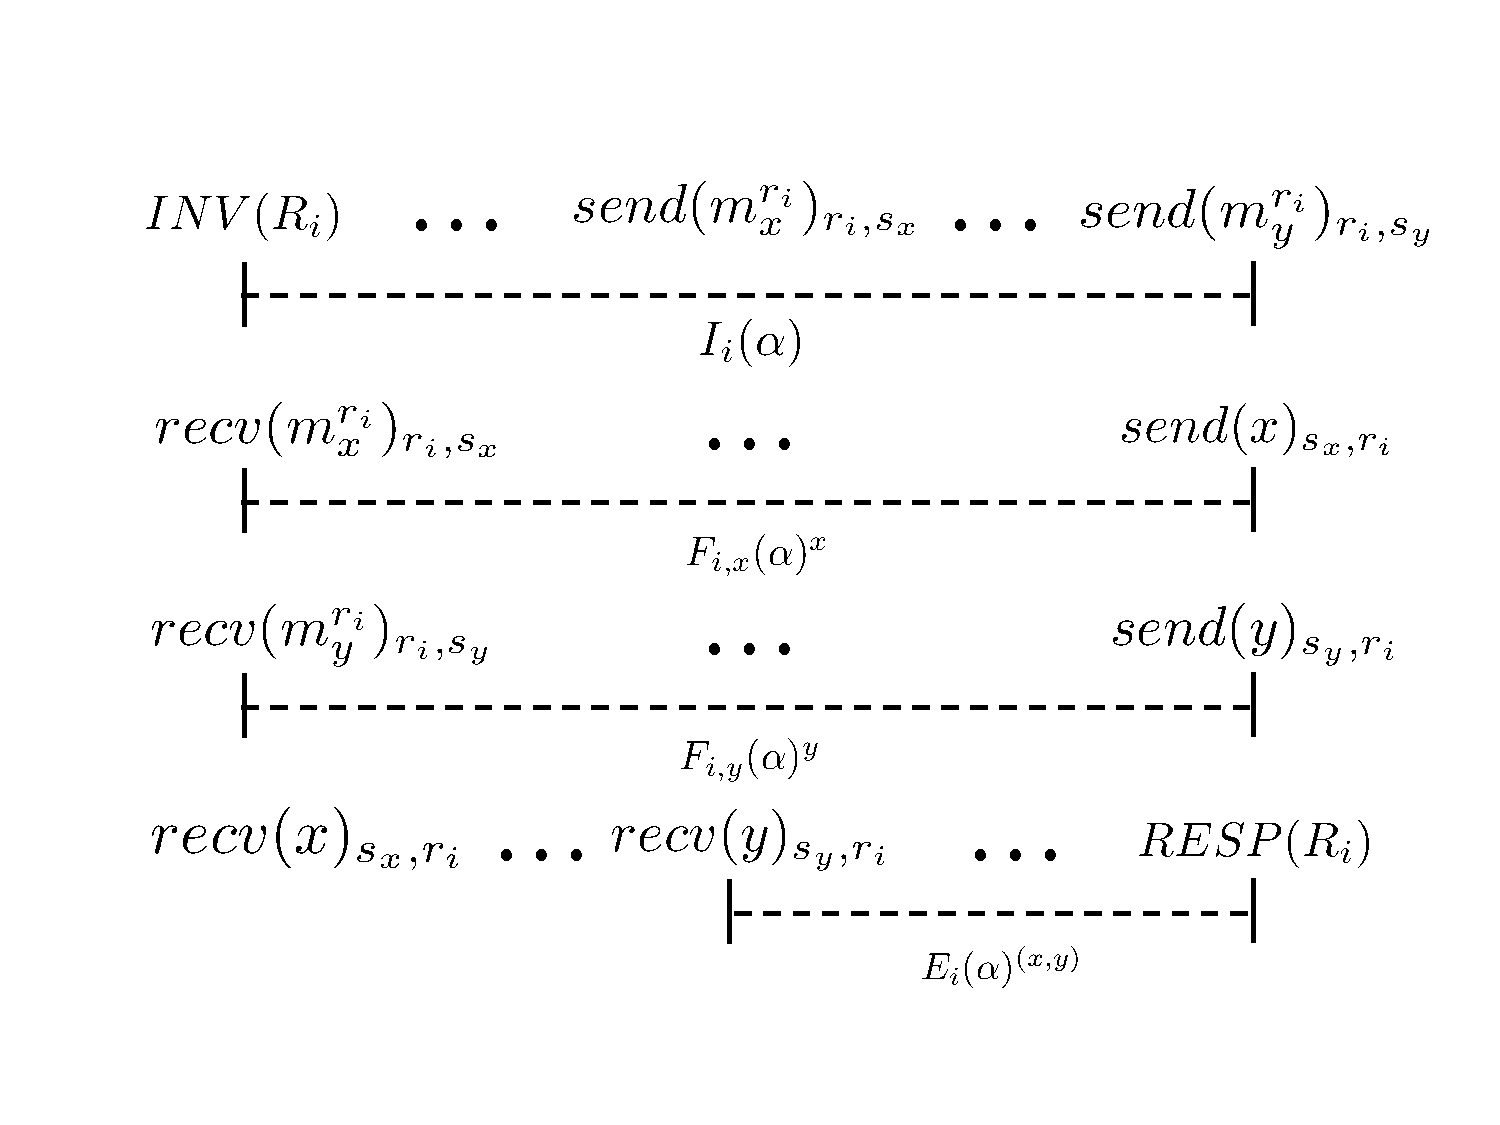
\includegraphics[scale=0.5]{figures/executions_3_2.pdf}
         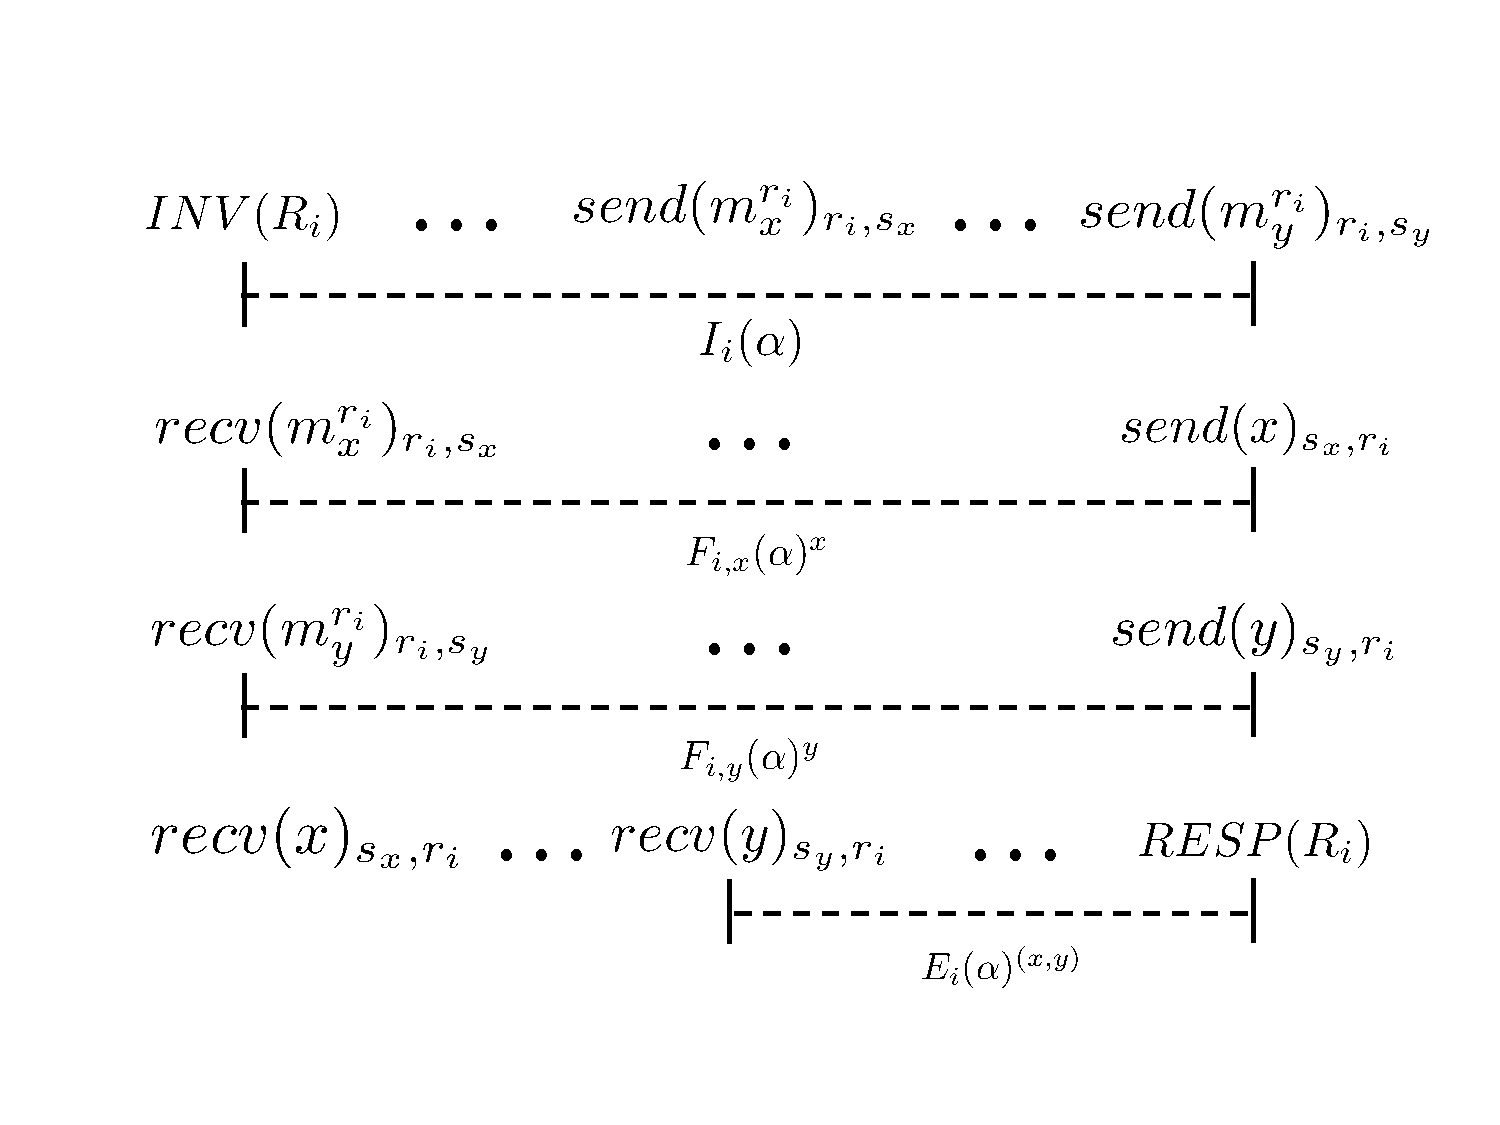
\includegraphics[width=4in]{figures/executions_3_2.png}
         \caption{
\small{The relevant actions in the execution fragments $I_i(\alpha)$, $F_{i,x}(\alpha)^{x}$,    $F_{i,y}(\alpha)^{y}$ and   $E_{i}(\alpha)^{(x,y)}$ for any \rot{} $R_i$, $i \in \{1, 2\}$
of a fair execution $\alpha$ of $\mathcal{A}$.}}
         \label{fig:exe3_fragments}
 \end{figure}
}

To play non-blocking fragments against the requirements of strict serializability and write isolation, we derive the following lemmas, which are frequently used by our proofs. In these lemmas, all \rots{} are assumed to have all SNOW properties, and we will derive contradictions in our main proofs. Due to space constraints, we explain these lemmas at a high level. %The proofs of these lemmas can be found in Appendix~\ref{app:lem_exec3_consistent}.

%We construct executions using \rots{} and \wots{} that always contact both servers $s_x$ and $s_y$.
%Because there is only one writer this makes objects $o_1$ and $o_2$ progress through versions together.
%This progression and strict serializability ensure that any \rot{} $R$ always returns the same version from both servers, e.g., $x_1$ and $y_1$.

%\wl{I'm not sure the purpose of the below paragraph now. Can we cut it out and just say the proof of the lemma is in the appendix? (I've cut it, but please confirm that's okay)}

%% Any  \rot{} $R$ initiated at a reader $r$, via the  
%% invocation action  $\INV{R}$ at $r$, after which the  actions $send(m_1^{r})_{r, s_x}$ and $send(m_2^{r})_{r, s_y}$, at $r$, send message $m_1^r$  to $s_x$ and $m_2^r$ to $s_y$, respectively. Once
%% $s_x$   receives $recv(m_1^{r})_{r, s_x}$  then  $s_x$ responds to $r$,  in a 
%% non-blocking manner,  with value $x$ via  action $send(x)_{s_x, r}$. Similarly,  after $s_y$  receives $m_2^{r}$ it  responds with $y$ to 
%% $r$ in a non-blocking manner via the action $send(y)_{s_y, r}$. After  $r$ receives $x$ and $y$ via actions $recv(x)_{s_x, r}$ and $recv(y)_{s_y, r}$, respectively,  $R$  completes
%%  with the response action $\RESP{R}$ and  returns $(x, y)$. 
%%
%% From the above discussion we can derive a lemma, which states in any  execution of $\mathcal{A}$,  if 
%% a server $s_i$  responds with a value $v_i$ during a   
%% \rot{}  then the \rot{} returns  
%% $v_i$ for  object $o_i$ and also, the pair of values $(x_t, y_t)$ are from some version $t$.
%% The result follows from the reliable channel model, where messages  reach at their destinations unaltered;  and by the S property  the object values, for objects $o_1$ and $o_2$,  returned by $R$  are of the same version.
%%
%% \wl{My cut of that paragraph ends here}
%%




%From the above discussion, it is easy to see that for any fair execution of $\mathcal{A}$ where $R_i$ is invoked, the adversary can always induce a fair execution of $\mathcal{A}$ where the fragments $I_i$, $\frage{F_{i,1}}{}{}$, $\frage{F_{i, 2}}{}{}$ and $E_i$ appear consecutively.
%Similarly, for any fair execution of  $\mathcal{A}$ where $R_2$ is invoked the adversary can always induce a fair execution of $\mathcal{A}$ where the fragments $I_2$, $\frage{F_{2,1}}{}{}$, $\frage{F_{2, 2}}{}{}$ and $E_2$ appear
  
%From this observation we can derive a lemma, which states in any execution of $\mathcal{A}$,  if 
%a server $s_i$ responds with a value $v_i$ during a   
%\rot{}  then the \rot{} returns  
%$v_i$ for  object $o_i$ and also, the pair of values $(x_t, y_t)$ are from some version $t$.
%The result follows from the reliable channel model, where messages reach at their destinations unaltered;  and by the S property  the object values, for objects $o_1$ and $o_2$,  returned by $R$  are of the same version.
The following lemma  proves that a \rot{} has to return the same version from both servers in order to satisfy strict serializability and write isolation.

\begin{lemma}\label{lem:exec3_consistent} 
Suppose $\alpha$ is any execution of $\mathcal{A}$ such that \rot{} $R$ is in $\alpha$. Suppose the  execution fragment $\frage{I}{\alpha}{} \circ \frage{F_{x}}{\alpha}{x_{t}} \circ \frage{F_{y}}{\alpha}{y_{s}} \circ \frage{E}{\alpha}{x_{t'}, y_{s'}}$ in $\alpha$, corresponds to $R$,  where   $x_t, x_{t'} \in V_1$ and  $y_s, y_{s'} \in V_2$, 
%then $(i)$ $s = s'$  and $ t=t'$ and $(ii)$ $s'=t'$.  
then $s=s'=t=t'$.  
%Similarly, if  the execution fragment $\frage{I_1}{\epsilon}{} \circ \frage{F_{2,1}}{\epsilon}{x} \circ \frage{F_{2,2}}{\epsilon}{y} \circ \frage{E_1}{\epsilon}{x', y'}$ appears, where   $x, x' \in V_1$ and  $y, y' \in V_2$, then $x = x'$ and $y=y'$.
\end{lemma}


%\wl{the removed proofs should all have pointers to their real proofs in the appendix, e.g., ``Proof given in Appendix~\ref{app:lem_exec3_consistent}''}

\remove{
\begin{proof}
Suppose $R$ is invoked at reader $r$.  Then, via the action $send(x_t)_{s_x, r}$, in 
execution fragment  $\frage{F_{1}}{\alpha}{x_{t}}$, server $s_x$ sends the value $x_t$ to $r$,   which is received at $r$ through the action 
$recv(x_{t'})_{s_x, r}$ in $\frage{E}{\alpha}{x_{t'}, y_{s'}}$.
 By the assumptions of the reliable channel automata in our model,  we have $x_{t}=x_{t'}$, i.e., $t=t'$. Similar argument for 
$\frage{F_{2}}{\alpha}{y_{s}}$  and $\frage{E}{\alpha}{x_{t'}, y_{s'}}$ leads us to conclude $s=s'$. Next, $R$ responds with $(x_{t'}, y_{s'})$, which implies  by the S property for executions of
 $\mathcal{A}$ that  $x_{t'}$ and $y_{s'}$ must correspond to the same version, i.e., $s'=t'$. %Therefore, we have $s = s' = t=t'$.
\end{proof}
}

%Note that the above results hold even if there are any other  execution fragments, that do not contain any actions at $r$, $s_x$ or $s_y$,   in-between the $I$, $F_i$ and $E$ execution  fragments. 

\remove{
\begin{corollary}\label{lem:exec3_consistent_corollary} 
Suppose $\alpha$ is any execution of $\mathcal{A}$ such that a \rot{} $R$ is in $\alpha$. Suppose the  execution fragment $\frage{I}{\alpha}{} \circ  X_1 \circ \frage{F_{1}}{\alpha}{x^{t}} \circ X_2 \circ  \frage{F_{2}}{\alpha}{y_{s}} \circ X_3 \circ \frage{E}{\alpha}{x_{t'}, y^{s'}}$ in $\alpha$,  corresponds to $R$,  where   $x_t, x_{t'} \in V_1$ and  $y^s, y^{s'} \in V_2$, $X_1, X_2, X_3$ are some execution fragments that do not contain any action at $r$, $s_x$ or $s_y$, and $s, s', t, t' $ are version identifiers  then $(i)$ $s = s'$  and $ t=t'$ and $(ii)$ $s'=t'$.  
\end{corollary}


\begin{proof} 
The constraint $(i)$ in the statement can be derived  from the fact that $\mathcal{A}$ satisfies the O property,  which implies that any version returned by $R$ for object value $o_1$ (or $o_2$) and this  must be the only version sent by the server $s_x$ (or $s_y$) to $r$. Constraint 
$(ii)$ from the S property of $\mathcal{A}$.
\end{proof}
}

%The following lemma states that new fair executions of $\mathcal{A}$ can be created by swapping execution fragments that  
%\blue{
%either $(a)$ have no input actions or 
%$(b)$ one of the fragments have no external (input or output) actions,
%}
% and in which   each fragment contains 
%actions that occur  only at one automaton and the automata for the two fragments are different. 
The following lemma states that we can create a new execution $\alpha'$ that is indistinguishable to $\alpha$ by swapping two fragments, which happen on two distinct automata in $\alpha$ if either $(a)$ both fragments have no input actions or 
$(b)$ one of the fragments have no external (input or output) actions. Our proofs leverage this lemma to create new executions by swapping such fragments and finally derive an execution that violates strict serializability.  
  \begin{lemma}[Commuting fragments] \label{lem:exec3_commute} 
  Let $\alpha$ be an execution of $\mathcal{A}$. Suppose $\frage{G_1}{\alpha}{}$ and $\frage{G_2}{\alpha}{}$ are any  execution fragments in $\alpha$ such that
  all actions in each fragment occur only at one automaton and  either $(a)$ none of the fragments contain input actions, or $(b)$ 
  at least one of the fragments have no external actions. Suppose $\frage{G_1}{\alpha}{}$ 
  and $\frage{G_2}{\alpha}{}$  occur at two distinct automata and the execution
  fragment $\frage{G_1}{\alpha}{}\circ \frage{G_2}{\alpha}{}$ occurs in $\alpha$.
  Then there exists an execution $\alpha'$ of $\mathcal{A}$, where  the execution fragment  $\frage{G_2}{\alpha}{}\circ \frage{G_1}{\alpha}{}$ appears in $\alpha'$, such that 
  %\blue{
  $(i)$  $\frage{G_1}{\alpha}{} \sim \frage{G_1}{\alpha'}{}$ and  $\frage{G_2}{\alpha}{} \sim \frage{G_2}{\alpha'}{}$
  %}
  $(ii)$ 
the prefix  in $\alpha$  before  $\frage{G_1}{\alpha}{} \circ \frage{G_2}{\alpha}{}$
 is identical to the prefix  in $\alpha'$ before  $\frage{G_1}{\alpha'}{} \circ \frage{G_2}{\alpha'}{}$; and $(ii)$ 
the suffix in $\alpha$  after   
 $\frage{G_1}{\alpha}{} \circ \frage{G_2}{\alpha}{}$
is identical to the suffix in $\alpha'$ after the execution fragment 
 $\frage{G_2}{\alpha'}{} \circ \frage{G_1}{\alpha'}{}$. 
 % Similar results  hold for the traces of $\alpha$ and $\beta$  in terms of the 
 %trace fragments   $\fragt{G_1}{\alpha}{}$ and $ \fragt{G_2}{\alpha}{}$
  \end{lemma}
 \remove{
  \begin{proof}
  This is clear because the adversary can move the actions in $G_2$ to occur before $G_1$ at their respective automata, and  because 
   either $(a)$ none of the fragments have any input action or $(b)$ at least one of them has no external actions, and hence 
  the actions in one of these fragments cannot affect the actions in the other fragment.
  \end{proof}
}


%The following lemma states that if there are two fair executions of $\mathcal{A}$ with a \rot{}  $R$ in each of them, and suppose at any server the non-blocking execution fragments  of $R$  are identical (in terms of the sequence of states and actions)  then in both executions, $R$   returns the same object value.
The following lemma states that if there are two fair executions of $\mathcal{A}$ with \rot{} $R$ in each of them, and suppose at any server the non-blocking fragments of $R$ are identical (in terms of the sequence of states and actions), then $R$ returns the same value in both executions.
\begin{lemma}[Indistinguishability]  \label{lem:exec3_equiv}
Let $\alpha$ and $\beta$ be executions of $\mathcal{A}$ and let $R$ be any \rot{}. Then 
$(i)$  if $\frage{F_{x}}{\alpha}{} \stackrel{s_x}{\sim}\frage{F_{x}}{\beta}{}$ then both 
$R(\alpha)$ and $R(\beta)$ respond with the same value $x$ at $s_x$; and 
$(ii)$ if  $\frage{F_{y}}{\alpha}{} \stackrel{s_y}{\sim}\frage{F_{y}}{\beta}{}$ then both 
$R(\alpha)$ and $R(\beta)$ respond with the same value $y$ at $s_y$.
\end{lemma}


\remove{
\begin{proof}
Suppose $R$ is invoked at some reader $r$. Let $j \in \{1, 2\}$ and  suppose the fragments  $\frage{F_{j}}{\alpha}{}$ and  $\frage{F_{j}}{\beta}{}$ 
appears in $\alpha$ and $\beta$ respectively, where in $\frage{F_{j}}{\alpha}{}$ server $s_j$
sends  $v_j \in V_j$ to $r$. Then $R(\alpha)$ must return $v_j$ for object $o_j$ by the O property  of $\mathcal{A}$. Then since $\frage{F_{j}}{\alpha}{} \stackrel{s_j}{\sim} \frage{F_{j}}{\beta}{}$ then
in  $\frage{F_{j}}{\beta}{}$  the server $s_j$ 
must also  send $v_j$ to $r$,  therefore,  both $R(\alpha)$ and $R(\beta)$ must return value $v_j$ for $o_j$.
%Then by the $S$ property  $R(\beta)$ must return $(x_t, y_t)$, which proves the result of the lemma. 
%
\end{proof}
}


%Below we show that in any finite execution of $\mathcal{A}$ where the final action is an invocation of  \rot{} $R$ at a reader $r$, the adversary can always induce a fair execution of $\mathcal{A}$ where the fragments $I$, $\frage{F_{1}}{}{}$, $\frage{F_{2}}{}{}$ and $E$ appear consecutively in that order.
 The following lemma shows that for any finite execution of $\mathcal{A}$ that ends with the invocation of  \rot{} $R_1$, it is always possible to have an execution of $\mathcal{A}$ where the fragments $I$, $\frage{F_{x}}{}{}$, $\frage{F_{y}}{}{}$ and $E$ appear consecutively due to the asynchronous network.
\begin{lemma}\label{lem:read_format}
%If a \rot{} $R_i$ is invoked in $\mathcal{A}$ then there exists a fair execution $\epsilon$ of $\mathcal{A}$ such that 
%the fragments $\frage{I_i}{\epsilon}{}$, $ \frage{F_{i, 1}}{\epsilon}{x}$, $\frage{F_{i, 2}}{\epsilon}{y}$ and 
 %$\frage{E_i}{\epsilon}{x, y}$ appear in $\epsilon$.
If any finite execution of  $\mathcal{A}$ ends with $\INV{R}$, for a \rot{} $R_1$ then there exists an extension $\alpha$ which is a fair execution of $\mathcal{A}$ and  is  of the form  
   $\frage{P}{\alpha}{} \circ\frage{I}{\alpha}{} \circ \frage{F_{1,x}}{\alpha}{x} \circ \frage{F_{1,y}}{\alpha}{y} \circ \frage{E}{\alpha}{x, y} \circ \frage{S}{\alpha}{}$, where $\frage{P}{\alpha}{}$ is the prefix and $\frage{S}{\alpha}{}$ denotes the rest of the execution. 
 \end{lemma}
 
 \remove{
 \begin{proof}
 Consider a finite execution of $\mathcal{A}$  that end with  $INV(R)$, which  occurs at some reader  $r$, 
then the  adversary  induces the execution fragment $\frage{I}{\alpha}{}$  by delaying all actions, except the internal and output actions at $r$, between 
the actions $\INV{R}$ and the later of the actions $send(m_1^{r})_{r, s_x}$ and $send(m_2^{r})_{r, s_y}$. Next, the adversary  
delivers $m_1^{r}$ at $s_x$ (via the action $recv(m_1^{r})_{r, s_x}$) and delays all actions, other than internal and output actions at $s_x$, until $s_x$ responds with $x$, via  $send(x)_{s_x, r}$; 
we identify this  execution fragment
 as $\frage{F_{1}}{\alpha}{x}$. Subsequently, in a similar manner, 
the  adversary  delivers the message  $m_2^{r}$ and delays appropriate actions to induce the execution fragment 
$\frage{F_{2}}{\alpha}{y}$. Finally, the adversary  delivers the values $x$ and $y$ to $r$ (via the events $recv(x)_{s_x, r}$ and $recv(y)_{s_y, r}$), 
and delays all actions at other automata until $R$ completes  with action $\RESP{R}$ by returning $(x, y)$.  As a result, we  arrive at a fair execution of $\mathcal{A}$ of the form
 $\frage{I}{\alpha}{} \circ \frage{F_{1}}{\alpha}{x} \circ \frage{F_{2}}{\alpha}{y} \circ \frage{E}{\alpha}{x, y} \circ \frage{S}{\alpha}{}$.
\end{proof}
}


\remove{
 \begin{figure}[t]
      \centering
         %\includegraphics[width=4.0in,  height=4in]{figures/executions_3_1-crop.pdf} 
        \includegraphics[scale=0.4]{figures/executions_3_1-crop.pdf} 
          %\vspace{-2.5em}
         \caption{
        \small{Executions of $\mathcal{A}$ with three clients and operations $W$, $R_1$ and $R_2$ leading to the contradiction of S in $\alpha_{10}$.
        Arrows show the transposition of execution fragments from the previous execution.
         % The external requests and responses  at the clients  to and from the end-users are represented as invocation and responses for the transaction.
         }} 
         \label{fig:executions3}
 \end{figure}
}

\begin{figure*}[t]
	%\centering
	\hspace*{-0.0cm}
	\begin{subfigure}{0.49\textwidth}
		\centering
	     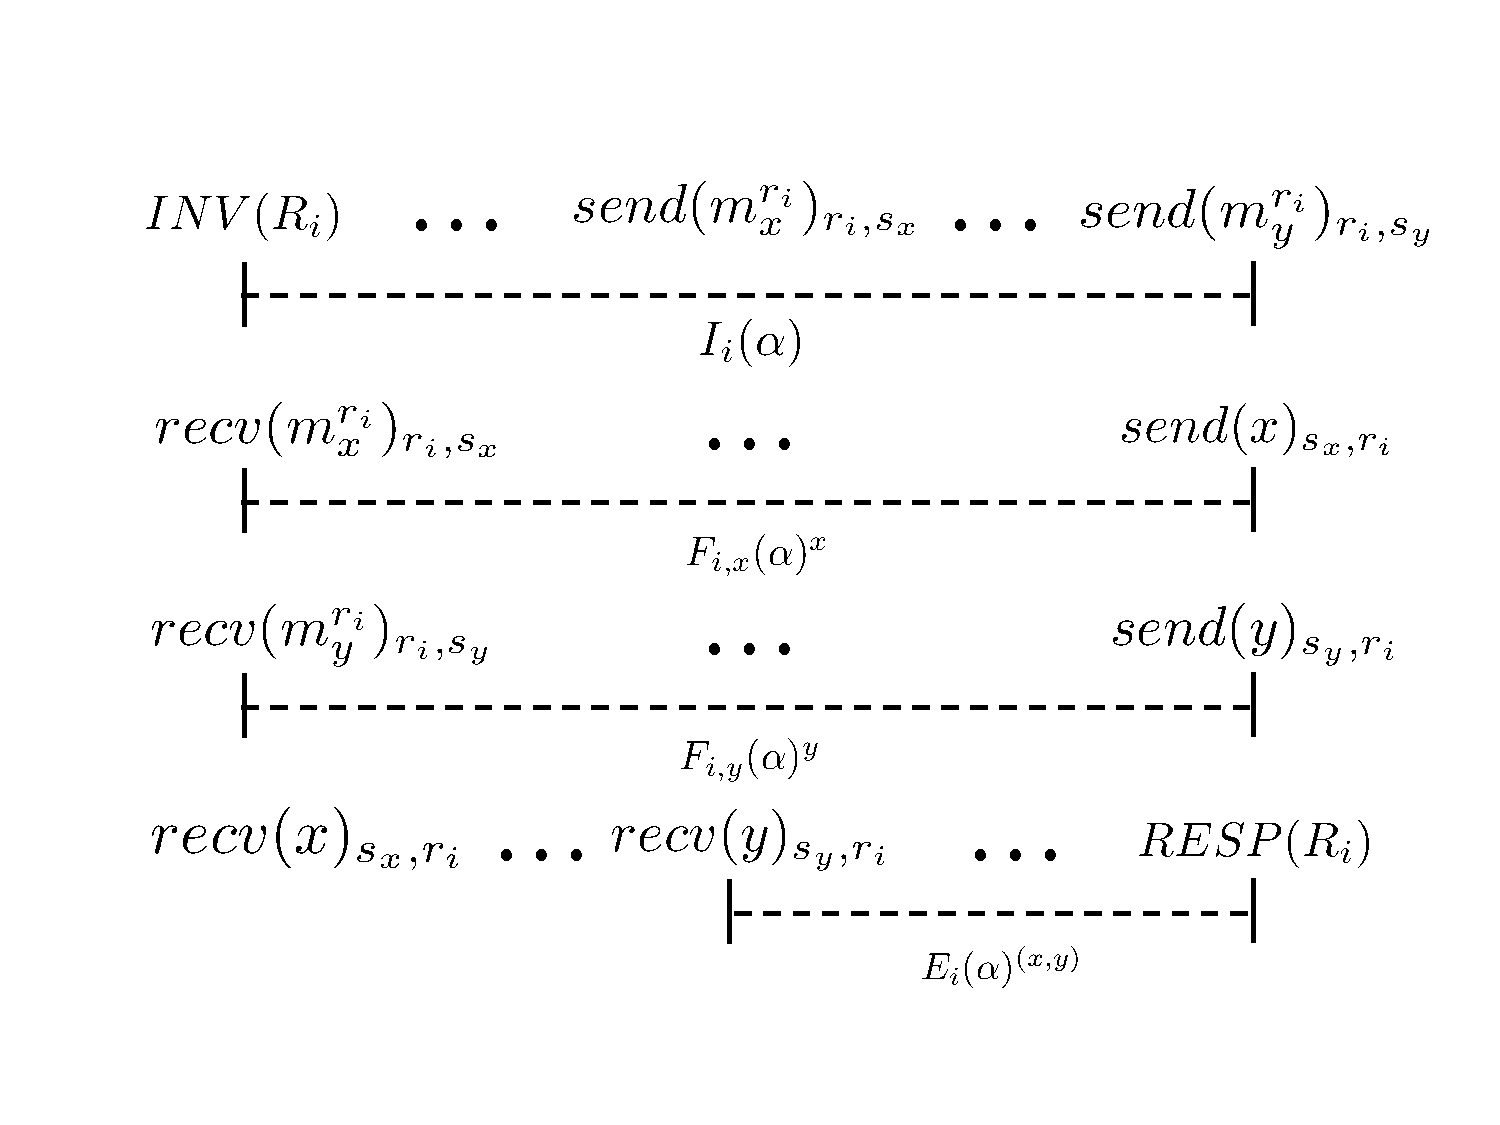
\includegraphics[width=3.0in]{figures/executions_3_2.pdf}
	     \caption{\small{
	      The relevant actions in the execution fragments $I_i(\alpha)$, $F_{i,x}(\alpha)^{x}$,    $F_{i,y}(\alpha)^{y}$ and   $E_{i}(\alpha)^{(x,y)}$ for any \rot{} $R_i$, $i \in \{1, 2\}$
			of a fair execution $\alpha$ of $\mathcal{A}$.
	     }}
	     \label{fig:exe3_fragments}
	\end{subfigure}
	\hspace*{0.0cm}  
	\begin{subfigure}{0.49\textwidth}
		\centering
		%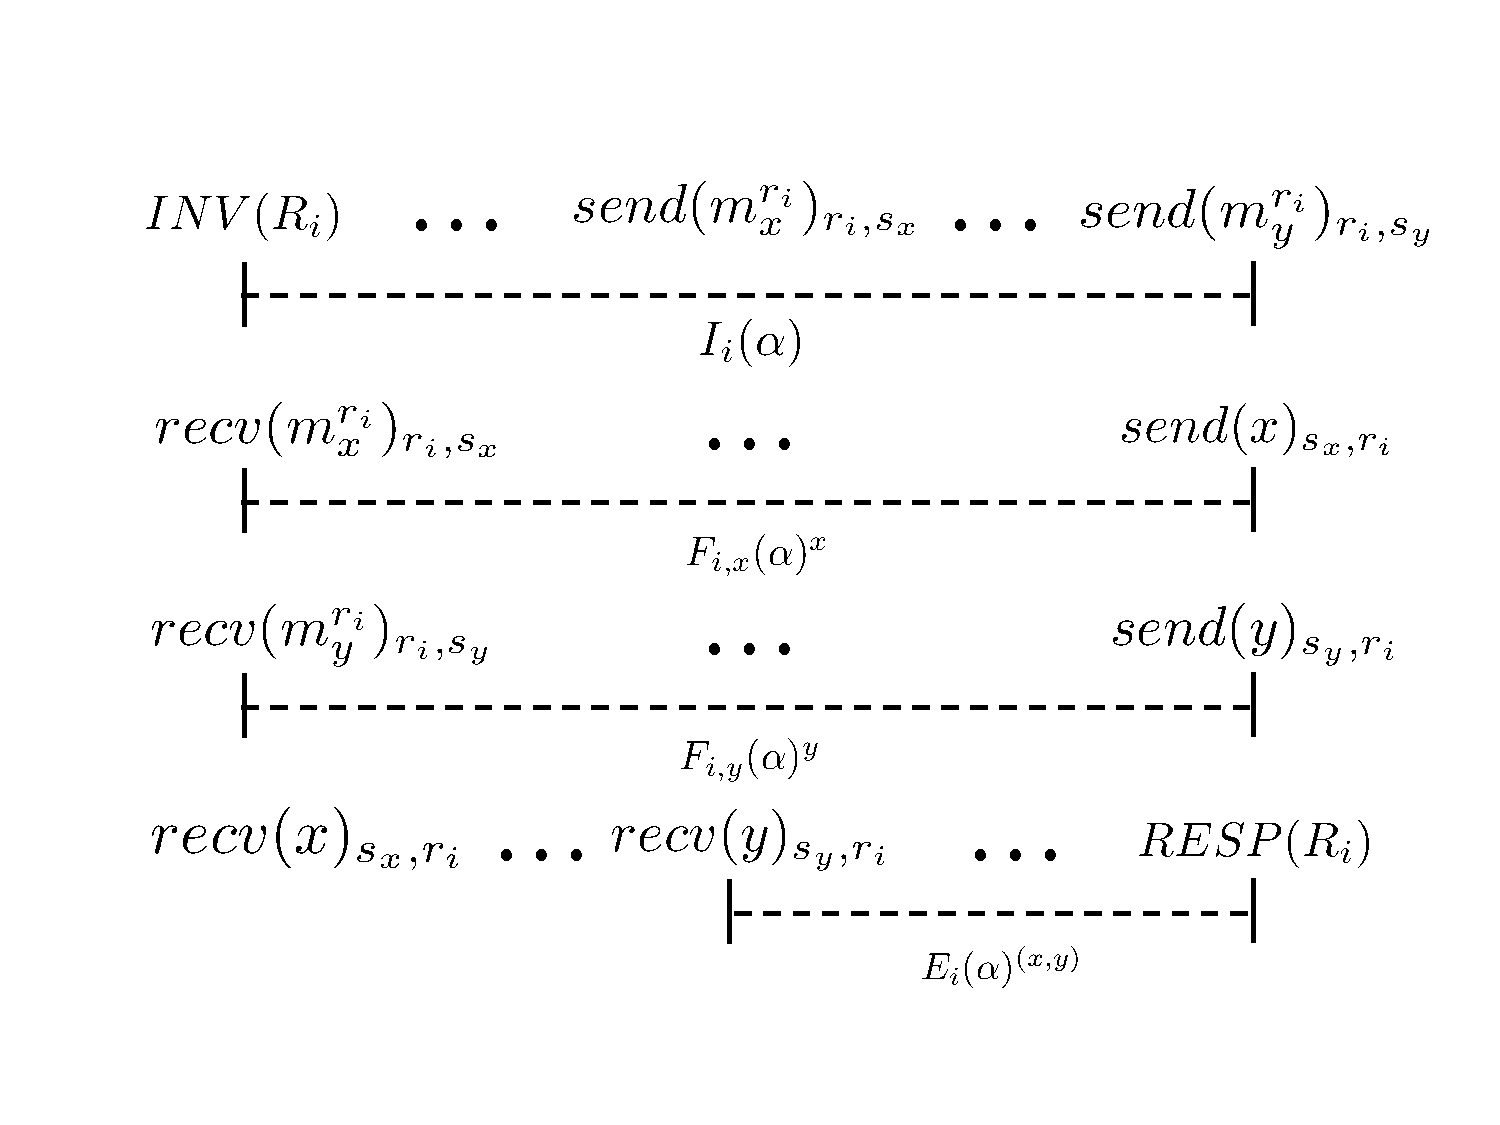
\includegraphics[width=3.2in]{figures/executions_3_2.pdf}		
		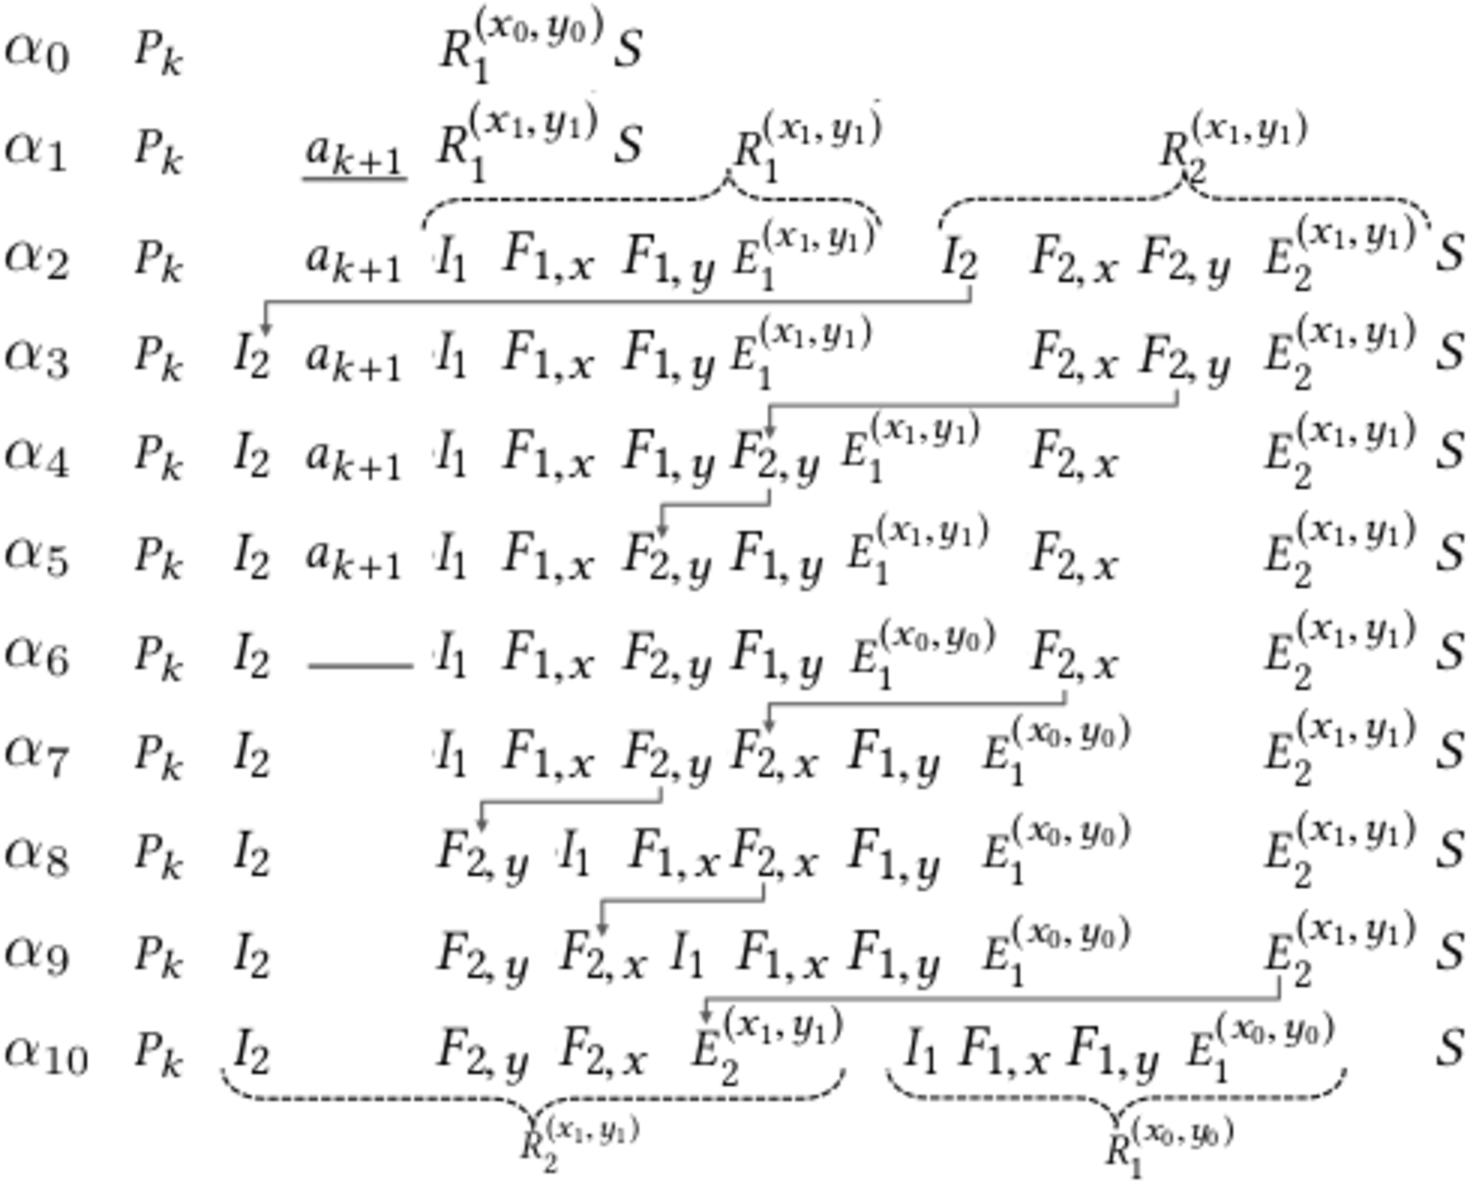
\includegraphics[width=3.0in]{figures/executions_3_1-cropa.pdf}		
		\caption{\small{Executions of $\mathcal{A}$ with three clients and operations $W$, $R_1$ and $R_2$ leading to the contradiction of S in $\alpha_{10}$.
			Arrows show the transposition of execution fragments from the previous execution.
		}}
           	\label{fig:executions3}
	\end{subfigure}   	
%\label{fig:executions3}		 
\end{figure*}

%\section{Impossibility of SNOW properties with  three clients}\label{three-client}
\section{No SNOW with Three Clients and C2C}
\label{sec:formal_proof}
\sloppy This section provides the sketch of a formal proof of the SNOW Theorem with 3 clients, i.e., SNOW is impossible in a system with 3 or more clients even when client-to-client communication is allowed. The main result of this section is captured by the following theorem. 
\begin{theorem}\label{thm:snow3}
	The SNOW properties cannot be implemented in a system with two readers and one writer, for two servers even in the presence of client-to-client communication.
\end{theorem}

Our proof strategy is to assume the existence of an algorithm $\mathcal{A}$ that satisfies all SNOW properties and create an execution $\alpha$ of $\mathcal{A}$ that contradicts the S property. 
We begin with an execution of $\mathcal{A}$ that contains \rots{} $R_1$ and $R_2$, which both read $s_x$ and $s_y$, and \wot{} $W$ that writes $(x_1, y_1)$ to $s_x$ and $s_y$ respectively (both servers have initial values $x_0$, $y_0$). $R_1$ begins after $W$ completes, and $R_2$ begins after $R_1$ completes. By the S property both  $R_1$   and $R_2$ should return $(x_1, y_1)$.
%First we show that any finite execution of $\mathcal{A}$ that ends with $\INV{R_i}$  has an extension which contains
%an execution fragment of the form
%$\frage{I}{\alpha}{} \circ \frage{F_{1}}{\alpha}{} \circ \frage {F_{2}}{\alpha}{} \circ \frage{E}{\alpha}{}$ that corresponds to $R_i$. 
Then we create a sequence of 
executions of $\mathcal{A}$  (Fig.~\ref{fig:executions3}), where we interchange the fragments until we  finally reach
 an execution in which $R_2$ completes before $R_1$ begins, but $R_2$ returns 
$(x_1, y_1)$ and $R_1$ returns $(x_0, y_0)$ which contradicts the  S property.

The following lemma shows that in an execution of $\mathcal{A}$ with a \wot{} $W$ and a \rot{} $R_1$, there exists a point  in the execution
such that if $R_1$ is invoked before that point then $R_1$ returns $(x_0, y_0)$ and if $R_1$ invoked after 
that point then $R_1$ returns $(x_1, y_1$).

\begin{lemma}[Existence of $\alpha_0$ and $\alpha_1$] \label{lem:exec3_alpha1} 
There exist  executions $\alpha_0$ and $\alpha_1$ of $\mathcal{A}$ that contain transactions $W$ and  $R_1$ 
%   with  the following properties:
that satisfy the following properties where $k$ is some positive integer and $\finiteprefixt{k-1}{k}$ is a prefix of $\finiteprefixt{k}{k+1}$:
$(i)$ $\alpha_0$ can be written as 
$\finiteprefixt{k-1}{k} \circ 
\frage{R_1}{\alpha_0}{x_0, y_0}
%\fragt{I_1}{\alpha_0}{} \circ \fragt{F_{1,x}}{\alpha_0}{x_0} \circ \fragt{F_{1,y}}{\alpha_0}{y_0} \circ \fragt{E_1}{\alpha_0}{x_0, y_0}
 \circ \frage{S}{\alpha_0}{}$ ;
 %and  $\beta_0$  as $\finiteprefixt{k-1}{k} \circ \fragt{R_1}{}{x_0, y_0} \circ \fragt{S}{\beta_0}{}$;
$(ii)$   $\alpha_1$ can be written as 
$\finiteprefixt{k}{k+1} \circ 
\frage{R_1}{\alpha_1}{x_1, y_1}  \circ \frage{S}{\alpha_1}{}$; and  
%$\beta_1$  as $\finiteprefixt{k}{k+1} \circ  \fragt{R_1}{}{x_1, y_1}
%\fragt{I_1}{\alpha_1}{} \circ \fragt{F_{1,x}}{\alpha_1}{x_1} \circ \fragt{F_{1,y}}{\alpha_1}{y_1}  \circ \fragt{E_1}{\alpha_1}{x_1, y_1} \circ \fragt{S}{\alpha_1}{}$; and 
$(iii)$ $a_{k+1}$ in $\alpha_1$  occurs at  $r_1$, 

%where $k$ is some positive integer and $\finiteprefixt{k-1}{k}$ is a prefix of $\finiteprefixt{k}{k+1}$.
%, i.e., the actions  $recv(m_x^r)_{r, s_x}$ and  $send(x)_{r, s_x}$ appear in $trace(\alpha)|s_x$, where  there is no input action of  $s_x$  between these actions.
% \item[$(ii)$]  $R(\alpha)$ returns  $(x_1, y_1)$. 
\end{lemma}

\begin{proof}
Now we describe the construction of a sequence  of finite executions of $\mathcal{A}$, $\{\gamma_k\}_{k=0}^{\infty}$  such that each $\gamma_k$ contains $W$ and $R_1$.
Consider an execution $\alpha$ of $\mathcal{A}$ that contains $W$. 
%Let us denote $\alpha$ as 
%$\finiteprefix{\ell}{\ell+1}\ldots$, where the  $\sigma$'s and the $a$'s are states and actions, of $\mathcal{A}$,  respectively, and $\ell$ is some positive integer. 
Suppose $R_1$ is invoked at $r_1$ after the execution fragment 
$\finiteprefixt{k}{k+1}$,  a
prefix of $\alpha$. Allowed by network asynchrony, let $\INV{R}$ be followed by only internal and external actions at $r_1$ until both
 $\send{m_x^{r_1}}{ r_1, s_x}$ and $\send{m_y^{r_1}}{ r_1, s_y}$ occur, thereby creating an execution fragment of the form
$\finiteprefixt{k}{k+1}\circ I_1(\alpha)$. We denote $\finiteprefixt{k}{k+1}$ by $\finiteprefixA{k}{k+1}$.

Next, consider the network delivers the message $m_x^{r_1}$ at $s_x$, and delays 
all actions at other automata and also any  input action at $s_x$ until $s_x$ sends $x$ to $r_1$. Therefore, we achieve the execution fragment   
$\finiteprefixA{k}{k+1}\circ \frage{ I_{1,x}}{\alpha}{} \circ \frage{F_{1,x}}{\alpha}{}$  of  ${\mathcal A}$. 
Next, the network delivers $m_y^{r_1}$ at $s_y$ and delays all actions at other automata and input actions at $s_y$ until $s_y$ sends $y$ to $r_1$. 
Then the network delivers $x$ and $y$ at $r_1$ but it delays  actions at other automata and any other input action at $r_1$ until $\RESP{R_1}$ occurs. Now we have an execution fragment of $\mathcal{A}$, which can be written as 
 $\finiteprefixA{k}{k+1}\circ \frage{I_1}{\alpha}{} \circ \frage{F_{1,x}}{\alpha}{x} \circ \frage{F_{1,y}}{\alpha}{y} \circ \frage{E_1}{\alpha}{x,y}$, where $R_1$ responds with $(x, y)$ such that $(x, y) \in \{ (x_0, y_0), (x_1, y_1) \}$.  We denote this finite execution prefix as $\gamma_k$. Therefore, there exists a sequence of such finite executions  
 $\{\gamma_k\}_{k=0}^{\infty}$.

Because $R_1$ precedes  $W$, by the S property $R_1$ must respond with $(x_0, y_0)$ in $\gamma_0$. If $k$ is large enough such that $a_{k}$ occurs in $\alpha$ after the completion of $W$ then by  the S property,  $R_1$ must return  $(x_1, y_1)$ in 
$\gamma_{k+1}$ due to the S property.  Therefore, there exists a minimum $k$  where in $\gamma_k$
\rot{} $R_1$ returns  $(x_0, y_0)$ and 
 in $\gamma_{k+1}$,
$R_1$ returns  $(x_1, y_1)$. 
%Note that here we used the fact that the version of both $x$ and $y$ change together due to the S property. 
Note that $\gamma_{k}$ corresponds to $\alpha_0$ and $\gamma_{k+1}$ corresponds to $\alpha_1$ in $(i)$ and $(ii)$ respectively. 

Now, we prove case $(iii)$ by eliminating the possibility of  $a_{k+1}$ occurring at $s_x$, $s_y$, $w$ or $r_2$.
% by showing contradictions.
%Our proof is based on the following argument. 
%
The S property requires that $R_1$ must return the same version from both $s_x$ and $s_y$, which implies that $s_x$ and  $s_y$ must send values of the same version.
%
%Note that for $R_1$, to respond with values for either version 
%$0$ or $1$, requires both $s_x$ and  $s_y$ to send object values of the same version, which is due to
% S property. 
%
Observe that $R_1$ returns the $0^{\textit{th}}$ version in $\alpha_0$ and the $1^{\textit{st}}$ version in $\alpha_1$,
 %$0$ (i.e., $(x_0, y_0)$)  and $1$ (i.e., $(x_1, y_1)$), respectively, 
 while the prefixes $\fragt{P_k}{\alpha_0}{}$ and 
 $\fragt{P_{k+1}}{\alpha_1}{}$ differ by a single action $a_{k+1}$. Importantly, just one action at any of  $s_x$, $s_y$, $r_2$
or $w$ is not enough for $s_x$ and $s_y$ to coordinate the same version to send. Therefore, $a_{k+1}$ must occur at $r_1$, which can 
possibly help coordinate by sending some information via $m_x$ and $m_y$ sent to $s_x$ and $s_y$ respectively.

\emph{ \underline{Case $a_{k+1}$ occurs at $s_x$}:} Consider the  prefix of execution $\alpha_0$ up to $a_k$.  Suppose the network invokes 
$R_1$ immediately after action $a_{k}$ via $\INV{R_1}$. By Lemma~\ref{lem:read_format} there exists  
an execution $\alpha'$ that contains an  execution fragment of the form
$\fragt{P_k}{\alpha'}{}
  \circ\frage{I_1}{\alpha'}{} \circ  \frage{F_{1,x}}{\alpha'}{x} 
  \circ\frage{F_{1,y}}{\alpha'}{y}
  \circ \frage{E}{\alpha'}{x, y}$.
Then, $\frage{I_1}{\alpha_1}{} \stackrel{r_1}{\sim} \frage{I_1}{\alpha'}{}$ and
  $\frage{F_{1,y}}{\alpha_1}{} \stackrel{s_y}{\sim} \frage{F_{1,y}}{\alpha'}{}$
  because in both executions the actions of $\frage{I_1}{}{}$ occur entirely at $r_1$
  and those of $\frage{F_{1,y}}{}{}$ occur entirely at $s_y$,
  and thus they are unaffected by the addition of the single action $a_{k+1}$ at $s_x$.  
As a result,  $\frage{F_{1,y}}{\alpha'}{}$ must send the same value $y_1$ to $r_1$ as 
 in  $\frage{F_{1,y}}{\alpha_1}{}$.
%
% at $s_x$ and 
%proceeds to time the delivery of messages so as to create an  execution fragment $\alpha'$,  of $\mathcal{A}$, with $\beta'$ of  the form 
%$\finiteprefixA{k-1}{k} \circ\fragt{I_1}{\alpha'}{} \circ  \fragt{F_{1,x}}{\alpha'}{} \circ\fragt{F_{1,y}}{\alpha'}{}$ such that, 
%$\frage{F_{1,y}}{\alpha_1}{} \stackrel{s_y}{\sim} \frage{F_{1,y}}{\alpha'}{}$. 
%This is possible because
%$\frage{I_1}{\beta}{} \circ  \fragt{F_{1,x}}{\beta}{}$ does not contain any input action at $s_y$.
Then in $\alpha'$, $R_1(\alpha')$ returns $y_1$ by Lemma~\ref{lem:exec3_equiv}, and thus $R_1(\alpha')$ returns $(x_1, y_1)$ by the 
S property. However, this contradicts the 
definition of $k$, i.e., the minimum value of $k$ such that $R_1$ responds with $(x_0, y_0)$.

\emph{ \underline{Case $a_{k+1}$ occurs at $s_y$}:} A  contradiction can be shown by following a line of reasoning similar to the  preceding case.

\emph{\underline{Case $a_{k+1}$ occurs at $w$}:}
This can be argued in a similar manner as the previous case with the trivial fact that $\frage{F_{1,x}}{\alpha_1}{} \stackrel{s_x}{\sim} \frage{F_{1,x}}{\alpha'}{}$ and $\frage{F_{1,y}}{\alpha_1}{} \stackrel{s_y}{\sim} \frage{F_{1,y}}{\alpha'}{}$.


\emph{\underline{Case $a_{k+1}$ occurs at $r_2$}:} 
A contradiction can be derived using a line of  reasoning as in the previous case.

So we conclude that $a_{k+1}$ must occur at $r_1$ in $\alpha_1$.
\end{proof}

In the remainder of the section, we suppress the explicit reference to the execution. For instance, we use $\fragt{I_i}{\alpha}{}$, $\fragt{F_{i,x}}{\alpha}{x}$, 
$\fragt{F_{i,y}}{\alpha}{y}$, $\fragt{E_i}{\alpha}{x, y}$ and $ \fragt{S}{\alpha}{}$, where we drop $\alpha$, 
instead of $\frage{I_i}{\alpha}{}$, $\frage{F_{i,x}}{\alpha}{x}$, 
$\frage{F_{i,y}}{\alpha}{y}$, $\frage{E_i}{\alpha}{x, y} $ and $ \frage{S}{\alpha}{}$.
%Moreover, for any execution $\alpha_i$ of 
%$\mathcal{A}$ we denote the trace $trace(\alpha_i)$ as $\beta_i$, and  for executions $\alpha$, $\alpha'$ and $\alpha''$ their corresponding traces  as $\beta$, $\beta'$ and $\beta''$, respectively. 
If a 
\rot{} $R_i$ has an  execution fragment of the form 
$\fragt{I_i}{\alpha}{} \circ \fragt{F_{i,x}}{\alpha}{x} \circ 
\fragt{F_{i,y}}{\alpha}{y} \circ \fragt{E_i}{\alpha}{x, y} $
we denote it  as  $\fragt{R_i}{}{x, y}$. 
%Also, whenever the returned values are unknown, clear from the context or irrelevant we omit them.
In the rest of the section, $\alpha_0$, $\alpha_1$, and the value of $k$ are the same as in the discussion above. We denote  the execution fragments  $\finiteprefixt{k}{k}$ and $\finiteprefixt{k}{k+1}$ as 
$\finiteprefixA{k}{k}$ and $\finiteprefixA{k}{k+1}$ respectively.
%, which are the same irrespective of the execution they appear in.

Our proof proceeds with a set of lemmas.  The first lemma states there exists an execution in which two consecutive \rots{} follow a \wot{}, and both \rots{}
return the new values by the \wot{}.

\begin{lemma}[Existence of $\alpha_2$] \label{lem:exec3_alpha2} 
\sloppy There exists an execution $\alpha_2$  of $\mathcal{A}$ that contains 
$W$, $R_1$, and $R_2$, and can be written in the form 
$\finiteprefixA{k}{k+1} \circ 
\frage{R_1}{}{x_1, y_1}
% \fragt{I_1}{\alpha_2}{} \circ  \fragt{F_{1,x}}{\alpha_2}{x_1} \circ \fragt{F_{1,y}}{\alpha_2}{y_1} \circ \fragt{E_1}{\alpha_2}{x_1, y_1}
 \circ
 \frage{R_2}{}{x_1, y_1}
 %\fragt{I_2}{\alpha_2}{}  \circ \fragt{F_{2,x}}{\alpha_2}{x_1} \circ \fragt{F_{2,y}}{\alpha_2}{y_1} \circ \fragt{E_2}{\alpha_2}{x_1, y_1}
\circ \fragt{S}{\alpha_2}{}$, where both $R_1$ and $R_2$ return $(x_1, y_1)$.
\end{lemma}

%\begin{proof}
%Presented in Appendix~\ref{app:sec5_lemmas}.
%\end{proof}

\remove{
\begin{proof}
We can construct an execution  $\alpha_2$ of $\mathcal{A}$ as follows. Consider the prefix 
$\finiteprefixt{k}{k+1} \circ 
\frage{R_1}{\alpha_1}{x_1, y_1}$
of the execution $\alpha_1$, from Lemma~\ref{lem:exec3_alpha1}. At the end of this prefix, the network invokes $R_2$. Now, by 
Lemma~\ref{lem:read_format}, due to $\INV{R_2}$
there is an extension of the prefix of the form 
$\finiteprefixt{k}{k+1} \circ  \frage{R_1}{\alpha_1}{x_1, y_1} \circ 
\frage{I}{\alpha}{} \circ \frage{F_{1}}{\alpha}{x} \circ \frage{F_{2}}{\alpha}{y} \circ \frage{E}{\alpha}{x, y}$. 
By the S property, we have $x = x_1$ and $y= y_1$. Therefore, $\alpha_2$ (Fig.~\ref{fig:executions3}) can be written in the form
$\finiteprefixA{k}{k+1} \circ 
\frage{R_1}{}{x_1, y_1}
% \fragt{I_1}{\alpha_2}{} \circ  \fragt{F_{1,x}}{\alpha_2}{x_1} \circ \fragt{F_{1,y}}{\alpha_2}{y_1} \circ \fragt{E_1}{\alpha_2}{x_1, y_1}
 \circ
 \frage{R_2}{}{x_1, y_1}
 %\fragt{I_2}{\alpha_2}{}  \circ \fragt{F_{2,x}}{\alpha_2}{x_1} \circ \fragt{F_{2,y}}{\alpha_2}{y_1} \circ \fragt{E_2}{\alpha_2}{x_1, y_1}
\circ \fragt{S}{\alpha_2}{}$, where $\fragt{S}{\alpha_2}{}$ is the rest of the execution.
%
\end{proof}
}

Based on the previous execution, the following lemma proves that there is an execution of 
$\mathcal{A}$ where $I_2$ occurs earlier than the action $a_{k+1}$ and the invocation of  $R_1$.
\begin{lemma}[Existence of $\alpha_3$] \label{lem:exec3_alpha3} 
\sloppy There exists  execution $\alpha_3$  of $\mathcal{A}$ that contains transactions $W$, $R_1$ and $R_2$, and can be written in the form  
$\finiteprefixA{k-1}{k} \circ  \fragt{I_2}{\alpha_3}{} \circ  a_{k+1} \circ 
\frage{R_1}{}{x_1, y_1}
%  \fragt{I_1}{\alpha_3}{} \circ \fragt{F_{1,x}}{\alpha_3}{x_1} \circ \fragt{F_{1,y}}{\alpha_3}{y_1} 
%\circ \fragt{E_1}{\alpha_3}{x_1, y_1}
\circ \fragn{F_{2,x}}{\alpha_3}{x_1} \circ \fragn{F_{2,y}}{\alpha_3}{y_1} \circ \fragn{E_2}{\alpha_3}{x_1, y_1}
\circ \fragt{S}{\alpha_3}{}$,  where both $R_1$ and $R_2$ return $(x_1, y_1)$.
\end{lemma}

%\begin{proof}
%Presented in Appendix~\ref{app:sec5_lemmas}.
%\end{proof}

%\remove{
\begin{proof}
Consider the execution $\alpha_2$ as in  Lemma~\ref{lem:exec3_alpha2}. 
In the execution fragment $ \fragt{I_1}{\alpha_2}{} \circ  \fragt{F_{1,x}}{\alpha_2}{x_1} \circ \fragt{F_{1,y}}{\alpha_2}{y_1} 
\circ \fragt{E_1}{\alpha_2}{x_1, y_1}$  in $\alpha_2$,  none of the actions occur at $r_2$ and  by Lemma~\ref{lem:exec3_alpha1}, $a_{k+1}$ occurs at $r_1$, 
also the actions in $\fragt{I_2}{}{}$ occur only at $r_2$.
%
Starting with $\alpha_2$, and by repeatedly using Lemma~\ref{lem:exec3_commute}, we create a sequence of four executions of $\mathcal{A}$ by repeatedly swapping 
 $\fragt{I_2}{\alpha_2}{}$ with the execution fragments 
$\fragt{E_1}{\alpha_2}{x_1, y_1}$, $\fragt{F_{1,y}}{\alpha_2}{y_1}$, $ \fragt{F_{1,x}}{\alpha_2}{x_1}$
and $\fragt{I_1}{\alpha_2}{}$, which appears in   $ \fragt{I_1}{\alpha_2}{} \circ  \fragt{F_{1,x}}{\alpha_2}{x_1} \circ \fragt{F_{1,y}}{\alpha_2}{y_1} 
\circ \fragt{E_1}{\alpha_2}{x_1, y_1}
\circ \fragt{I_2}{\alpha_2}{}$, 
where the following sequence of execution fragments
 $ \fragt{I_1}{\alpha_2}{} \circ  \fragt{F_{1,x}}{\alpha_2}{x_1} \circ \fragt{F_{1,y}}{\alpha_2}{y_1}  \circ \fragt{I_2}{\alpha_2}{} \circ \fragt{E_1}{\alpha_2}{x_1, y_1}$ (by commuting  $\fragt{I_2}{\alpha_2}{}$  and $\fragt{E_1}{\alpha_2}{x_1, y_1}$); ~
 $ \fragt{I_1}{\alpha_2}{} \circ  \fragt{F_{1,x}}{\alpha_2}{x_1} \circ \fragt{I_2}{\alpha_2}{}  \circ \fragt{F_{1,y}}{\alpha_2}{y_1} \circ \fragt{E_1}{\alpha_2}{x_1, y_1}$ (by commuting $\fragt{I_2}{\alpha_2}{}$  and $\fragt{F_{1,y}}{\alpha_2}{y_1}$); ~
 $ \fragt{I_1}{\alpha_2}{} \circ  \fragt{I_2}{\alpha_2}{}  \circ \fragt{F_{1,x}}{\alpha_2}{x_1} \circ \fragt{F_{1,y}}{\alpha_2}{y_1} \circ \fragt{E_1}{\alpha_2}{x_1, y_1}$ (by commuting   $\fragt{I_2}{\alpha_2}{}$  and $\fragt{F_{1,x}}{\alpha_2}{x_1}$)
appear. Finally, we have an  execution $\alpha'$ of the form 
$ \finiteprefixA{k}{k+1} \circ  \fragt{I_2}{\alpha''}{} \circ 
\frage{R_1}{}{x_1, y_1}
%  \fragt{I_1}{\alpha_3'}{} \circ \fragt{F_{1,x}}{\alpha_3'}{x_1} \circ \fragt{F_{1,y}}{\alpha_3'}{y_1} 
%\circ \fragt{E_1}{\alpha_3'}{x_1, y_1}
\circ \fragt{F_{2,x}}{\alpha'}{x_1} \circ \fragt{F_{2,y}}{\alpha'}{y_1} \circ \fragt{E_2}{\alpha_3'}{x_1, y_1}
\circ \fragt{S}{\alpha'}{}$ (by commuting $\fragt{I_2}{\alpha_2}{}$ and $\fragt{I_1}{\alpha_2}{}$)
Next, from $\alpha'$, by using Lemma~\ref{lem:exec3_commute}  and swapping $a_{k+1}$ with $\fragt{I_2}{\alpha_2}{}$ 
we have shown the existence  of  an execution 
 $\alpha_3$.
\end{proof}
%}

\remove{
In the following lemma, we show that we can create an execution $\alpha_4$ of $\mathcal{A}$, where 
$\fragt{F_{2,y}}{\alpha_4}{}$ occurs immediately before  $ \fragt{E_1}{\alpha_4}{x_1, y_1}$, while $\fragt{R_1}{\alpha_4}{}$ and 
$\fragt{R_2}{\alpha_4}{}$ both return 
$(x_1, y_1)$.
\begin{lemma}[Existence of $\alpha_4$] \label{lem:exec3_alpha4} 
\sloppy There exists  execution $\alpha_4$  of $\mathcal{A}$ that contains transactions $W$, $R_1$ and $R_2$ and  can be written in the form
$ \finiteprefixA{k-1}{k} \circ \fragt{I_2}{\alpha_4}{}  \circ a_{k+1} $$ \circ \fragt{I_1}{\alpha_4}{}
\circ \fragn{F_{1,x}}{\alpha_4}{x_1} \circ   \fragn{F_{1,y}}{\alpha_4}{y_1} 
\circ \fragn{F_{2,y}}{\alpha_4}{y_1} 
\circ \fragn{E_1}{\alpha_4}{x_1, y_1}
$$\circ \fragn{F_{2,x}}{\alpha_4}{x_1} \circ  \fragn{E_2}{\alpha_4}{x_1, y_1}\circ \fragt{S}{\alpha_4}{}$, where both $R_1$ and $R_2$ return $(x_1, y_1)$.
\end{lemma}
}

%\begin{proof}
%Presented in Appendix~\ref{app:sec5_lemmas}.
%\end{proof}

\remove{
\begin{proof}
We start with an execution  $\alpha_3$, as in  Lemma~\ref{lem:exec3_alpha3}, and apply Lemma~\ref{lem:exec3_commute} twice.  

First, by  Lemma~\ref{lem:exec3_commute}, we know there exists an execution $\alpha'$ of $\mathcal{A}$
where  $\fragt{F_{2,x}}{\alpha_3}{}$ (identify as $G_1$) and 
$\fragt{F_{2,y}}{\alpha_3}{}$ (identify as $G_2$)  are interchanged since actions of 
$\fragt{F_{2,x}}{\alpha_3}{}$ occurs solely at $s_x$ and those of $\fragt{F_{2,y}}{\alpha_3}{}$ at $s_y$, 
and  $\fragt{F_{2,x}}{\alpha_3}{}$ and $\fragt{F_{2,y}}{\alpha_3}{}$ return $x_1$ and $y_1$, respectively, to $r_2$.


Next, by Lemma~\ref{lem:exec3_commute} there is 
execution  of $\mathcal{A}$,  say $\alpha_4$ where
the fragments 
$\fragt{E_1}{\alpha_3}{}$ (identify as $G_1$)  and 
$\fragt{F_{2,y}}{\alpha_3}{}$ (identify as $G_2$) are interchanged, with respect to $\alpha'$, because  the actions in  $\fragt{E_1}{\alpha'}{}$ occur at $r_1$ and 
those of $\fragt{F_{2,y}}{\alpha_3}{}$ at $s_y$. Furthermore, $\alpha_4$
  can be written in the form
 $  \finiteprefixA{k-1}{k}  \circ  \fragt{I_2}{\alpha''}{} \circ  a_{k+1}  \circ $$
  \fragt{I_1}{\alpha''}{} \circ \fragt{F_{1,x}}{\alpha''}{x_1}
   \circ \fragt{F_{1,y}}{\alpha''}{y_1} 
  \circ \fragt{F_{2,y}}{\alpha''}{y_1} 
\circ \fragt{E_1}{\alpha''}{x_1, y_1}
\circ \fragt{F_{2,x}}{\alpha''}{x_1} \circ \fragt{E_2}{\alpha''}{x_1, y_1}
\circ \fragt{S}{\alpha''}{}$.
\end{proof}
}


\remove{
 Next, we create an execution  $\alpha_5$ where 
    $\fragt{F_{2,y}}{\alpha_5}{}$ occurs before  $ \fragt{F_{1,y}}{\alpha_5}{}$. 
    %However, because the actions in both execution fragments occur at the same automaton care has to be taken to swap these fragments 
    %compared to $\alpha_4$.
%\blue{

\begin{lemma}[Existence of $\alpha_5$] \label{lem:exec3_alpha4b} 
\sloppy There exists  execution $\alpha_5$  of $\mathcal{A}$ that contains transactions $W$, $R_1$ and $R_2$ and  can be written in the form
$ \finiteprefixA{k-1}{k} \circ \fragt{I_2}{\alpha_5}{}  \circ a_{k+1} $$ \circ \fragt{I_1}{\alpha_5}{}
\circ \fragn{F_{1,x}}{\alpha_5}{x_1} \circ \fragn{F_{2,y}}{\alpha_5}{y_1} \circ  \fragn{F_{1,y}}{\alpha_5}{y_1} \circ \fragn{E_1}{\alpha_5}{x_1, y_1}
$$\circ \fragn{F_{2,x}}{\alpha_5}{x_1} \circ  \fragn{E_2}{\alpha_5}{x_1, y_1}\circ \fragt{S}{\alpha_5}{}$, 
where both $R_1$ and $R_2$ return $(x_1, y_1)$.
\end{lemma}

%}
}
\remove{
\begin{proof}
%\blue{
Given all actions  in $ \fragt{F_{1,y}}{\alpha_4}{} $ and 
  $\fragt{F_{2,y}}{\alpha_4}{}$ occur at $s_y$ in $\alpha_4$, consider the prefix of $\alpha_4$ that ends with $\fragn{F_{1,x}}{\alpha''}{x_1}$. We extend this prefix as follows.
In this prefix,  the actions $send(m_y^{r_2})_{r_2, s_y}$ and 
 $send(m_y^{r_1})_{r_1, s_y}$ do not have their corresponding $recv$ actions.  Suppose  the network 
delivers $m_y^{r_2}$ at $s_y$ (via the action $recv(m_y^{r_2})_{r_2, s_y}$) and delays all actions, other than internal and output actions at $s_y$, until $s_y$ responds with $y$, via  action $send(y)_{s_y, r_2}$. This extended execution fragment is of the form $\fragt{F_{2,y}}{\alpha_4}{}$. Similarly, the network further extends the execution by placing  the 
action $recv(m_y^{r_1})_{r_1, s_y}$ at $s_y$  and creates the execution fragment of the form $\fragt{F_{1,y}}{\alpha_4}{}$. Note that, so far, the actions due to the above extensions are entirely at $s_y$. Suppose the network makes the execution 
fragments $\fragt{E_1}{\alpha''}{}$ happen next by delivering values sent during $\fragt{F_{1,x}}{\alpha_4}{}$ and $\fragt{F_{1,y}}{\alpha_4}{}$ via the actions  $recv(x)_{s_x, r_1}$ and $recv(y)_{s_y, r_1}$ respectively at $r_1$. Then $\fragt{F_{2,x}}{\alpha''}{}$ occurs next, such that this fragment contains exactly the same sequence of actions as  in the corresponding execution fragment in  $\alpha_4$.
This is possible because they are not influenced by  any output action in $\fragt{F_{2,y}}{\alpha_4}{}$  or $\fragt{F_{1,y}}{\alpha_4}{}$. 
Suppose the network places the execution fragment  $\fragt{E_2}{\alpha''}{}$ next.
Let us denote the execution that is an extension of this finite execution so far as $\alpha_5$, which is of the form $ \finiteprefixA{k-1}{k} \circ \fragt{I_2}{\alpha_5}{}  \circ a_{k+1} $$ \circ \fragt{I_1}{\alpha_5}{}
\circ \fragt{F_{1,x}}{\alpha_5}{} \circ \fragt{F_{2,y}}{\alpha_5}{} \circ  \fragt{F_{1,y}}{\alpha_5}{} \circ \fragt{E_1}{\alpha_5}{}
$$\circ \fragt{F_{2,x}}{\alpha_5}{} \circ  \fragt{E_2}{\alpha_5}{}\circ \fragt{S}{\alpha_5}{}$.
 Now we need to argue about the values returned by the reads.
 %}
 
 %\blue{
Note that both $\alpha_4$ and $\alpha_5$ have the same execution fragment  $\frage{F_{1,x}}{\alpha_4}{}$. Therefore,   $\frage{F_{1,x}}{\alpha_4}{} \stackrel{s_x}{\sim} \frage{F_{1,x}}{\alpha_5}{}$, and thus $s_x$ also returns $x_1$ in $\fragt{F_{1,x}}{\alpha_4}{}$ in $\alpha_5$. Next  by Lemma~\ref{lem:exec3_equiv} for $R_1$,  $s_y$ returns $y_1$ in $\fragt{F_{1,y}}{\alpha_5}{}$  and  hence by the S property, $R_1(\alpha_5)$ returns $(x_1, y_1)$, i.e.,   that $r_1$ returns the new version of object values. Therefore, $\frage{F_{1,x}}{\alpha_4}{}$,  $\fragt{F_{1,y}}{\alpha_5}{}$ and $\fragt{E_1}{\alpha_5}{}$ are of the form $ \fragt{F_{1,x}}{\alpha_5}{x_1}$, $\fragt{F_{1,y}}{\alpha_5}{y_1}$ and  $\fragt{E_1}{\alpha_5}{x_1, y_1}$, respectively.
%}

%\blue{
Note that by construction of $\alpha_5$ above,  the execution fragment  $\fragt{F_{2,x}}{\alpha_4}{}$ in both $\alpha_4$ and $\alpha_5$ is the same, therefore,   $\frage{F_{2,x}}{\alpha_4}{} \stackrel{s_x}{\sim} \frage{F_{2,x}}{\alpha_5}{}$. Hence as in 
$\alpha_4$,  $s_x$  returns $x_1$  in the execution fragment  $\frage{F_{2, 1}}{\alpha_5}{}$  in   $\alpha_5$,  i.e.,  of the form $\frage{F_{2, 1}}{\alpha_5}{x_1}$.
Since $s_x$ returns $x_1$ in $\fragt{F_{2, 1}}{\alpha_5}{}$ in $\alpha_5$,  by   
Lemma~\ref{lem:exec3_equiv}  and   the S property,
  $R_2$ returns $(x_1, y_1)$  and hence $\fragt{E_2}{\alpha_5}{}$ is of the form $\fragt{E_2}{\alpha_5}{x_1, y_1}$.
%}

%\blue{
From the above argument we know that  $\alpha_5$ is of the form $ \finiteprefixA{k-1}{k} \circ \fragt{I_2}{\alpha_5}{}  \circ a_{k+1} $$ \circ \fragt{I_1}{\alpha_5}{}
\circ \fragt{F_{1,x}}{\alpha_5}{x_1} \circ \fragt{F_{2,y}}{\alpha_5}{y_1} \circ  \fragt{F_{1,y}}{\alpha_5}{y_1} \circ \fragt{E_1}{\alpha_5}{x_1, y_1}
$$\circ \fragt{F_{2,x}}{\alpha_5}{x_1} \circ  \fragt{E_2}{\alpha_5}{x_1, y_1}\circ \fragt{S}{\alpha_5}{}$.
%}
\end{proof}
}
\remove{
In the next lemma, we show the existence of an execution of $\mathcal{A}$ where $R_1$ returns $(x_0, y_0)$  and $I_2$ occurs immediately after $a_{k}$ and 
 $R_2$ responds with $(x_1, y_1)$. 
%In fact, this is the most important of the sequence of executions of  
%$\mathcal{A}$  (Fig.~\ref{fig:executions3})  because later with this  we prove in Theorem~\ref{thm:snow3} the existence of a
%execution of $\mathcal{A}$ where a \rot{} returns object-values of an earlier version compared to a previous \rot{} that is not
%concurrent with it.
\begin{lemma}[Existence of $\alpha_6$] \label{lem:exec3_alpha5} 
\sloppy There exists  execution $\alpha_6$  of $\mathcal{A}$ that contains transactions $W$, $R_1$ and $R_2$ and can be
written in the form 
$ \finiteprefixA{k-1}{k} \circ\fragt{I_2}{\alpha_6}{} \circ  \fragt{I_1}{\alpha_6}{} \circ\fragn{F_{1,x}}{\alpha_6}{x_0}
\circ\fragn{F_{2,y}}{\alpha_6}{y_1}\circ \fragn{F_{1,y}}{\alpha_6}{y_0} \circ\fragn{E_1}{\alpha_6}{x_0, y_0}
\circ\fragn{F_{2,x}}{\alpha_6}{x_1} \circ \fragn{E_2}{\alpha_6}{x_1, y_1}\circ \fragt{S}{\alpha_6}{}$, 
where  $R_1$ returns $(x_0, y_0)$  and $R_2$ returns $(x_1, y_1)$.
\end{lemma}

\begin{proof}
The crucial part of this proof is to carefully use the result of  Lemma~\ref{lem:exec3_alpha1} so that $R_1$ returns $(x_0, y_0)$, instead of $(x_1, y_1)$.
Note that the same prefix $\finiteprefixA{k-1}{k}$ appears in $\alpha_5$ of Lemma~\ref{lem:exec3_alpha4b} as well as in $\alpha_0$ and $\alpha_1$ of Lemma~\ref{lem:exec3_alpha1}, where
 $k$ is defined as in Lemma~\ref{lem:exec3_alpha1}.

By Lemma~\ref{lem:exec3_alpha1}, action $a_{k+1}$ occurs at $r_1$.
 In the execution fragment 
 $a_{k+1} $$ \circ \fragt{I_1}{\alpha_5}{}
\circ \fragt{F_{1,x}}{\alpha_5}{x_1} \circ \fragt{F_{2,y}}{\alpha_5}{y_1}$ of $\alpha_5$, the actions in
 $a_{k+1} $$ \circ \fragt{I_1}{\alpha_4}{}$ occur at $r_1$; actions in 
$\fragt{F_{1,x}}{\alpha_4}{x_1}$ occur at $s_x$; and  actions in $\fragt{F_{2,y}}{\alpha_4}{y_1}$ occur at $s_y$. 
Now consider the  prefix of execution $\alpha_4$ ending with $I_2$ and the network invokes $R_1$ immediately after $I_2$  (instead of 
after $a_{k+1}$) and  extends it by the execution fragment  $ \fragt{I_1}{\epsilon}{} \circ \fragt{F_{1,x}}{\epsilon}{} \circ  \fragt{F_{2,y}}{\epsilon}{}$ to create a new finite execution $\epsilon$, which is of the form $\finiteprefixA{k-1}{k}  \circ \fragt{I_2}{\epsilon}{} \circ \fragt{I_1}{\epsilon}{} \circ \fragt{F_{1,x}}{\epsilon}{} \circ  \fragt{F_{2,y}}{\epsilon}{}$. As a result, $a_{k+1}$ may not be in $\epsilon$ because we introduce changes before $a_{k+1}$ occurs.

Note  that if  in the prefix
 $\finiteprefixA{k-1}{k}  \circ \frage{I_2}{\epsilon}{} \circ \frage{I_1}{\epsilon}{} \circ \frage{F_{1,x}}{\epsilon}{} \circ  \frage{F_{2,y}}{\epsilon}{}$  of $\epsilon$ 
we ignore the actions in $\frage{I_2}{\epsilon}{}$
 then the remaining execution is the same as the prefix  
 $\finiteprefixA{k-1}{k}  \circ  \frage{I_1}{\alpha_0}{} \circ \frage{F_{1,x}}{\alpha_0}{} \circ  \frage{F_{2,y}}{\alpha_0}{}$ of $\alpha_0$ in 
Lemma~\ref{lem:exec3_alpha1}. Here we explicitly use the notations $\epsilon$ and $\alpha_0$ to avoid confusion. Since the actions in 
$\frage{I_2}{\epsilon}{}$ have no impact on the actions in 
 $\frage{I_1}{\epsilon}{} \circ \frage{F_{1,x}}{\epsilon}{} \circ  \frage{F_{2,y}}{\epsilon}{}$,
we have $\frage{F_{1,x}}{\epsilon}{} \stackrel{s_x}{\sim} \frage{F_{1,x}}{\alpha_0}{}$. Therefore, by Lemma~\ref{lem:exec3_consistent} 
  $\frage{F_{1,x}}{\epsilon}{}$ returns $x_0$ as in  $\frage{F_{1,x}}{\alpha_0}{}$, i.e., $s_x$ returns $x_0$ in $\fragn{F_{1,x}}{\epsilon}{x_0}$. 
Now by Lemma~\ref{lem:exec3_equiv} we  conclude that 
%Then, by Lemma~\ref{lem:exec3_alpha1}, 
for  any  extension of $\epsilon$, say $\gamma$, \rot{} 
 $R_1(\gamma)$ returns $x_0$ at $s_x$ and by the S property  $R_1(\gamma)$ returns  $(x_0, y_0)$. Also, since 
$\frage{F_{2,y}}{\alpha_5}{} \stackrel{s_y}{\sim} \frage{F_{2,y}}{\epsilon}{} \stackrel{s_y}{\sim} \frage{F_{2,y}}{\gamma}{}$  by Lemma~\ref{lem:exec3_equiv} and the S property,  $R_2(\gamma)$ must return $(x_1, y_1)$.  Therefore, $\gamma$ has an extension of $\alpha_6$ (Fig.~\ref{fig:executions3}) which is of  the form $ \finiteprefixA{k-1}{k}  \circ\fragt{I_2}{\alpha_6}{} \circ  \fragt{I_1}{\alpha_6}{} \circ\fragt{F_{1,x}}{\alpha_6}{x_0}
\circ\fragt{F_{2,y}}{\alpha_6}{y_1}\circ \fragt{F_{1,y}}{\alpha_6}{y_0} \circ\fragt{E_1}{\alpha_6}{x_0, y_0}
\circ\fragt{F_{2,x}}{\alpha_6}{x_1} \circ \fragt{E_2}{\alpha_6}{x_1, y_1}\circ \fragt{S}{\alpha_6}{}$ as in the statement of the lemma.
\end{proof}
}
\remove{
The  following lemma shows that there exists  an execution $\alpha_7$ for $\mathcal{A}$ where $\fragt{F_{2,x}}{\alpha_7}{}$ 
appears  before $\fragn{F_{1,y}}{\alpha_7}{y_0} \circ\fragn{E_1}{\alpha_7}{x_0, y_0}$, where $R_1$ returns $(x_0, y_0)$ and $R_2$ returns $(x_1, y_1)$.  The lemma can be proven by  starting from $\alpha_6$ in Lemma~\ref{lem:exec3_alpha5} and  moving the execution fragments  of $R_2$ earlier, a little at a time, until finally we have $R_2$ finishing before $R_1$ starts.  This simply uses commutativity since the actions in the swapped execution fragments occur at different automata.

%\wl{Is the preceeding paragraph describing just lemma 5.7, or the rest of the proof, or some combination of both. I cannot tell. Please update the text to make it clear.}

\begin{lemma}[Existence of $\alpha_7$] \label{lem:exec3_alpha6} 
\sloppy There exists  execution $\alpha_7$  of $\mathcal{A}$ that contains transactions $W$, $R_1$ and $R_2$, and   can be written in the form
$\finiteprefixA{k-1}{k} \circ \fragt{I_2}{\alpha_7}{}  \circ \fragt{I_1}{\alpha_7}{} \circ \fragn{F_{1,x}}{\alpha_7}{x_0} 
\circ \fragn{F_{2,y}}{\alpha_7}{y_1}\circ \fragn{F_{2,x}}{\alpha_7}{x_1} 
 \circ \fragn{F_{1,y}}{\alpha_7}{y_0} \circ\fragn{E_1}{\alpha_7}{x_0, y_0}\circ
 \fragn{E_2}{\alpha_7}{x_1, y_1}\circ \fragt{S}{\alpha_7}{}$ where $R_1$ returns $(x_0, y_0)$ and $R_2$ returns $(x_1, y_1)$.
\end{lemma}
}

\remove{
\begin{proof}
\sloppy This result is proved by applying the result of Lemma~\ref{lem:exec3_commute}  to the execution created in Lemma~\ref{lem:exec3_alpha5}. 
Suppose,  $\alpha_6$ (Fig.~\ref{fig:executions3}) is a  execution as  in Lemma~\ref{lem:exec3_alpha5}, 
where in  the   execution fragment 
$\fragt{E_1}{\alpha_6}{x_0, y_0}\circ\fragt{F_{2,x}}{\alpha_6}{}$  we identify 
 $\fragt{E_1}{\alpha_6}{x_0, y_0}$  as $G_1$ and 
$\fragt{F_{2,x}}{\alpha_6}{y_0}$  as $G_2$. The actions of $G_1$ and $G_2$ occur at two distinct automata, therefore,  we  can use the result of Lemma~\ref{lem:exec3_commute}, to argue that there exists an execution $\alpha'$ of $\mathcal{A}$  that  contains the  execution fragment 
$\fragt{F_{2,x}}{\alpha_7}{}  \circ\fragt{E_1}{\alpha_7}{x_0, y_0}$, and $\alpha_6$ and $\alpha'$ are identical in the prefixes and suffixes corresponding to $G_1$ and $G_2$.

 Now,  $\alpha'$ contains  $\fragt{F_{1,y}}{\alpha''}{} \circ \fragt{F_{2,x}}{\alpha'}{}$, where  
  the actions in  $\fragt{F_{1,y}}{\alpha''}{}$ (identified as $G_1$) and $\fragt{F_{2,x}}{\alpha''}{}$ (identify as $G_2$)  occur  at distinct automata. Hence, by  Lemma~\ref{lem:exec3_commute} there exists  an execution $\alpha_7$ of the form
$\finiteprefixA{k-1}{k}  \circ \fragt{I_2}{\alpha_7}{}  \circ \fragt{I_1}{\alpha_7}{} \circ \fragt{F_{1,x}}{\alpha_7}{x_0} 
\circ \fragt{F_{2,y}}{\alpha_7}{y_1}\circ \fragt{F_{2,x}}{\alpha_7}{x_1} 
 \circ \fragt{F_{1,y}}{\alpha_7}{y_0} \circ\fragt{E_1}{\alpha_7}{x_0, y_0}\circ
 \fragt{E_2}{\alpha_7}{x_1, y_1}\circ \fragt{S}{\alpha_7}{}$.
%
\end{proof}
}

\remove{
The following lemma leverages Lemma~\ref{lem:exec3_commute} to show the existence of an execution $\alpha_8$ of $\mathcal{A}$ where $\fragt{F_{2,y}}{\alpha_8}{}$ appears before $\fragt{I_1}{\alpha_8}{} \circ \fragt{F_{1,x}}{\alpha_8}{}$, and $R_1$ returns $(x_0, y_0)$ while $R_2$ returns $(x_1, y_1)$.

\begin{lemma} [Existence of $\alpha_8$]  \label{lem:exec3_alpha7} 
\sloppy There exists  execution $\alpha_8$  of $\mathcal{A}$ that contains transactions $W$, $R_1$ and $R_2$
and   can be written in the form 
$\finiteprefixA{k-1}{k}  \circ  \fragt{I_2}{\alpha_8}{} \circ \fragn{F_{2,y}}{\alpha_8}{y_1} \circ 
$$\fragt{I_1}{\alpha_8}{} \circ \fragn{F_{1,x}}{\alpha_8}{x_0} 
\circ  \fragn{F_{2,x}}{\alpha_8}{x_1} 
$$ \circ \fragn{F_{1,y}}{\alpha_8}{y_0} \circ \fragn{E_1}{\alpha_8}{x_0, y_0}
\circ \fragn{E_2}{\alpha_8}{x_1, y_1}\circ \fragt{S}{\alpha_8}{}$, where $R_1$ returns $(x_0, y_0)$ and $R_2$ returns $(x_1, y_1)$.
\end{lemma}
}


\remove{
\begin{proof}
 Consider the execution $\alpha_7$ of $\mathcal{A}$ as in Lemma~\ref{lem:exec3_alpha6}. In the context of 
  of  Lemma~\ref{lem:exec3_commute}, in $\alpha_7$ (Fig.~\ref{fig:executions3}) the actions in  
 $ \fragt{F_{1,x}}{\alpha_8}{}$ (identify as $G_1$)  occur at $s_x$  and  those in $\fragt{F_{2,y}}{\alpha_8}{}$ (identify as $G_2$) at  $s_y$. Then by  
 Lemma~\ref{lem:exec3_commute} there exists an execution $\alpha'$ of $\mathcal{A}$,  of the form 
 $ \finiteprefixA{k-1}{k}  \circ \fragt{I_2}{\alpha'}{}  \circ \fragt{I_1}{\alpha''}{} 
 \circ \fragn{F_{2,y}}{\alpha'}{y_1} 
\circ \fragn{F_{1,x}}{\alpha'}{x_0} 
\circ \fragn{F_{2,x}}{\alpha'}{x_1} 
 \circ \fragn{F_{1,y}}{\alpha'}{y_0} \circ\fragn{E_1}{\alpha'}{x_0, y_0}\circ
 \fragn{E_2}{\alpha''}{x_1, y_1}\circ \fragt{S}{\alpha'}{}$, where $ \fragt{F_{2,y}}{\alpha_8}{}$ and 
  $ \fragt{F_{1,x}}{\alpha_8}{}$  are interchanged.
 
 Since  actions in  $ \fragt{F_{2,y}}{\alpha_8}{}$ (identify as $G_1$)  occur at $s_y$ and those in 
  $ \fragt{I_{1}}{\alpha_8}{}$ (identify as $G_1$)  occur at $r_1$ then by Lemma~\ref{lem:exec3_commute}
  there is a  execution of $\mathcal{A}$, $\alpha_8$ where $\fragt{F_{2,y}}{\alpha_8}{}$ appear before $\fragt{I_1}{\alpha_8}{}$, i.e., of the form  $\finiteprefixA{k-1}{k}  \circ \fragt{I_2}{\alpha_8}{} \circ \fragt{F_{2,y}}{\alpha_8}{}  \circ
 \fragt{I_1}{\alpha_7}{} \circ \fragt{F_{1,x}}{\alpha_8}{} 
\circ \fragt{F_{2,x}}{\alpha_8}{} 
 \circ \fragt{F_{1,y}}{\alpha_8}{} \circ\fragt{E_1}{\alpha_8}{} \circ
 \fragt{E_2}{\alpha_8}{}\circ \fragt{S}{\alpha_8}{}$, where $ \fragt{F_{2,y}}{\alpha_8}{}$ and 
  $ \fragt{I_{1}}{\alpha_8}{}$  are interchanged.
 
 By $(ii)$ of Lemma~\ref{lem:exec3_equiv} we have 
$\frage{F_{2,x}}{\alpha'}{} \stackrel{s_x}{\sim} \frage{F_{2,x}}{\alpha_8}{}$ hence $\fragt{F_{2,x}}{\alpha_8}{}$ sends $x_1$ and 
$\fragt{F_{1,x}}{\alpha_8}{}$ and $\fragt{F_{1,y}}{\alpha_8}{}$ sends $x_0$ and $y_0$, respectively. So considering these returned values we have $\alpha_8$ 
(Fig.~\ref{fig:executions3}) in the form as stated in the lemma.
\end{proof}
}

%\wl{Please replace all language ``forward past'' with ``earlier than'', which is much clearer about where things are moving. I think i have fixed all of these.}
\remove{
The following lemma shows the existence of an execution  $\alpha_9$, of $\mathcal{A}$, where 
$\fragt{F_{2,x}}{}{}$ appears before $\fragt{F_{1,x}}{}{}$.
%\blue{
\begin{lemma} [Existence of $\alpha_9$]  \label{lem:exec3_alpha8} 
\sloppy There exists  execution $\alpha_9$  of $\mathcal{A}$ that contains transactions $W$, $R_1$ and $R_2$
and   can be written in the form 
$\finiteprefixA{k-1}{k}  \circ  \fragt{I_2}{\alpha_8}{} \circ \fragt{F_{2,y}}{\alpha_8}{y_1} \circ 
$$\fragt{I_1}{\alpha_8}{} \circ \fragt{F_{2,x}}{\alpha_8}{x_1} 
\circ  \fragt{F_{1,x}}{\alpha_8}{x_0} 
$$ \circ \fragt{F_{1,y}}{\alpha_8}{y_0} \circ \fragt{E_1}{\alpha_8}{x_0, y_0}
\circ \fragt{E_2}{\alpha_8}{x_1, y_1}\circ \fragt{S}{\alpha_8}{}$
where $R_1$ returns $(x_0, y_0)$ and $R_2$ returns $(x_1, y_1)$.
\end{lemma}
%}
}
\remove{
\begin{proof}
%\blue{
In $\alpha_8$ from Lemma~\ref{lem:exec3_alpha7}, all the actions in  
 $ \fragn{I_1}{\alpha_8}{}$  occur at $r_1$; those in   $ \fragn{F_{1,x}}{\alpha_8}{x_1}$  occur at $s_x$; and  the  
actions in $ \fragn{F_{2,x}}{\alpha_8}{y_1}$ occur only  at $s_x$. 
%
Note that actions of  both execution fragments $ \fragt{F_{2,x}}{\alpha_8}{}$  and   
$\fragt{F_{1,x}}{\alpha_8}{}$ occur at $r_1$.  
Consider the prefix of $\alpha_8$ that ends with $\fragt{I_1}{}{}$ then suppose the network  extends this prefix by adding an execution fragment of the form
$ \fragt{F_{2,x}}{\alpha_8}{} \circ  \fragt{F_{1,x}}{\alpha_8}{}$ as follows.  
%
First note that  the actions $send(m_x^{r_2})_{r_2, s_x}$ and 
 $send(m_x^{r_1})_{r_1, s_x}$ appears in the prefix but do not have corresponding $recv$ actions.
 %}
%\blue{
The  network places action $recv(m_x^{r_2})_{r_2, s_x}$, and allows an execution fragment of the form 
$ \fragt{F_{2,x}}{\alpha_8}{}$ to appear. Now, immediately after this the network further extends it with 
an execution fragment of the form  $\fragt{F_{1,x}}{\alpha_8}{}$  by placing action $recv(m_x^{r_1})_{r_1, s_x}$. 
 Next the fragment $\fragn{F_{1,y}}{\alpha_8}{y_0}$ is added  and is the same as $ \frage{F_{1,y}}{\alpha_8}{}$.
This last step can be argued by the fact that none of the actions in  $ \fragn{F_{1,y}}{\alpha_8}{y_0}$ can be affected by 
any of the output actions at $ \fragt{F_{2,x}}{\alpha_8}{}$ and  $\fragt{F_{1,x}}{\alpha_8}{}$. Note that a careful argument can be done by using Theorem~\ref{thm:fairtrace} to conclude the same. Following this the network allows the rest of the execution by adding an execution fragment of the form $\fragn{E_1}{\alpha_8}{x_0, y_0}
\circ \fragn{E_2}{\alpha_8}{x_1, y_1}\circ \fragn{S}{\alpha_8}{}$. The resulting execution is of the form 
$\finiteprefixA{k-1}{k}  \circ  \fragt{I_2}{\alpha_8}{} \circ \fragt{F_{2,y}}{\alpha_8}{y_1} \circ 
$$\fragt{I_1}{\alpha_8}{} \circ \fragn{F_{2,x}}{\alpha_8}{x_1} 
\circ  \fragn{F_{1,x}}{\alpha_8}{x_0} 
$$ \circ \fragt{F_{1,y}}{\alpha_8}{y_0} \circ \fragn{E_1}{\alpha_8}{x_0, y_0}
\circ \fragn{E_2}{\alpha_8}{x_1, y_1}\circ \fragt{S}{\alpha_8}{}$, where we retained the values wherever it is known, and we denote this  execution by $\alpha_9$.
%}

%\blue{
Now, we argue about the return values in $\alpha_9$. 
Applying Lemma~\ref{lem:exec3_equiv} to $R_2$ and $\fragn{F_{2,y}}{\alpha_8}{y_1}$ implies that $R_2$ 
returns $(x_1, y_1 )$. Similarly, 
applying Lemma~\ref{lem:exec3_equiv} to $R_1$ and $\fragn{F_{1,y}}{\alpha_8}{y_0}$ implies that $R_1$ 
must return $(x_0, y_0 )$ in $\alpha_9$.
%}
\end{proof}
}

%\wl{below should be ``where $R_1$ returns $(x_0, y_0)$ and $R_2$ completes by returning $(x_1, y_1)$'' I think! (the first $R_2$ should be a $R_1$.)}

Now we realize the existence of an execution $\alpha_{10}$  of $\mathcal{A}$ where the execution fragments corresponding to $R_2$ appears 
before $R_1$, where  $R_1$ returns $(x_0, y_0)$ and $R_2$ completes by returning $(x_1, y_1)$
but $R_1$ is in real time after $R_2$, therefore, violates the S property.
%\blue{
\begin{lemma} [Existence of $\alpha_{10}$]  \label{lem:exec3_alpha11} 
\sloppy There exists an execution $\alpha_{10}$  of $\mathcal{A}$ that contains transactions $W$, $R_1$ and $R_2$
and   can be written in the form 
$\finiteprefixA{k-1}{k}   \circ
\frage{R_2}{}{x_1, y_1} \circ
 \frage{R_1}{}{x_0, y_0}
 \circ \fragt{S}{\alpha_{10}}{}$.
where $R_1$ returns $(x_0, y_0)$ and $R_2$ returns $(x_1, y_1)$.
\end{lemma}
%}
\begin{proof}
%\blue{
Now, by applying Lemma~\ref{lem:exec3_commute} to $\alpha_{9}$, we can swap 
 $\fragt{F_{2,x}}{}{}$  and $ \fragt{I_1}{}{}$ to create an execution $\alpha_{10}$  (Fig.~\ref{fig:executions3}) of $\mathcal{A}$, which is
of the form 
$ \finiteprefixA{k-1}{k}   \circ 
\fragt{I_2}{\alpha_9}{} \circ \fragt{F_{2,y}}{\alpha_9}{y_1} 
\circ   \fragt{F_{2,x}}{\alpha_9}{x_1}  \circ 
\frage{R_1}{}{x_0, y_0} \circ \fragt{E_2}{\alpha_8}{x_1, y_1}
%\fragt{I_1}{\alpha_9}{} \circ \fragt{F_{1,x}}{\alpha_9}{x_0}  \circ \fragt{F_{1,y}}{\alpha_9}{y_0} \circ \fragt{E_1}{\alpha_9}{x_0, y_0}\circ \fragt{E_2}{\alpha_9}{x_1, y_1}
 \circ \fragt{S}{\alpha_9}{}$, where the returned values are determined by  Lemma~\ref{lem:exec3_consistent}.
 %}
 
%\blue{
Note that none of the actions in 
$\fragt{I_1}{\alpha_9}{} \circ \fragt{F_{1,x}}{\alpha_9}{x_0} 
 \circ \fragt{F_{1,y}}{\alpha_9}{y_0} \circ \fragt{E_1}{\alpha_9}{x_0, y_0}$
occur at $r_2$ and all actions in $\fragt{E_2}{\alpha_9}{x_1, y_1} $ occur at $r_2$. Therefore, by 
applying Lemma~\ref{lem:exec3_commute}, we can consecutively swap $\fragt{E_2}{}{}$ with 
%
$\fragt{E_1}{}{}$, $\fragt{F_{1,y}}{}{}$,  $\fragt{I_1}{}{}$,  and $\fragt{F_{1,x}}{}{}$. Therefore, we create a sequence of 
four executions of $\mathcal{A}$ to arrive at execution $\alpha_{10}$ (Fig.~\ref{fig:executions3}) of the form
$\finiteprefixA{k-1}{k}   \circ
\frage{R_2}{}{x_1, y_1}
 %\fragt{I_2}{\alpha_10}{} \circ \fragt{F_{2,y}}{\alpha_10}{y_1} 
%\circ   \fragt{F_{2,x}}{\alpha_10}{x_1}  \circ \fragt{E_2}{\alpha_10}{x_1, y_1} \circ
%\fragt{I_1}{\alpha_10}{} \circ \fragt{F_{1,x}}{\alpha_10}{x_0} 
 % \fragt{F_{1,y}}{\alpha_10}{y_0} \circ \fragt{E_1}{\alpha_10}{x_0, y_0}
 \circ
 \frage{R_1}{}{x_0, y_0}
 \circ \fragt{S}{\alpha_{10}}{}$.
%}
\end{proof}
\remove{
Using the above results,  we prove Theorem ~\ref{thm:snow3} for 3-clients by showing the existence of $\alpha_{10}$,  where $R_2$ completes before $R_1$ is invoked and  $R_2$ returns $(x_1, y_1)$ whereas $R_1$ returns $(x_0, y_0)$, which  violates the S property. 
}
%\begin{proof}
\sloppy 
%Therefore, $\alpha_{10}$ (shown in Fig.~\ref{fig:executions3}) provides an execution, where $R_1$ returns $(x_0, y_0)$ and $R_2$ returns $(x_1, y_1)$, but $R_1$ is in real time after $R_2$, therefore, violates the S property.
%\end{proof}

\setcounter{algorithm}{3}


%\section{Impossibility of SNOW properties with two clients with restricted communication }\label{two-client}
\section{Two Client Open Question}
\label{sec:2c2s}
This section closes the open question of whether SNOW properties can be implemented with two clients. We first prove that SNOW remains impossible in a 2-client 2-server system if the clients cannot directly send messages to each other.
% We prove our result by showing 
 %a contradiction. 
 However, in the presence of client to client communication, it is possible to have all SNOW properties with two clients and at least two servers.
 %Fig~\ref{fig:architecture2a}.
 
 \subsection{No  SNOW Without C2C  Messages}
 \label{subsec:no_snow_no_c2c}
 
 
 In this section, we prove the following results that states it is impossible guarantee the SNOW properties in a transaction processing system with two clients, without client-to-client communication.
  \begin{theorem}\label{thm:two-snow}
  	The SNOW properties cannot be implemented in a system with two clients and two servers, where the clients do not communicate with each other.
  \end{theorem} 
 
 We use the same system model as in Section~\ref{sec:formal_proof}: two servers $s_x$ and $s_y$ with two clients, a reader $r_1$ that issues only 
\rots{} and a writer $w$ that issues only \wots{}. A \wot{} $W$ writes $(x_1, y_1)$ to $s_x$ and $s_y$, and a \rot{} $R$ reads both servers. We assume that there is a bi-directional communication channel between any pair of client and server and any pair of servers. There is no communication channel between clients. We assume that each transaction can be identified by a unique number, e.g., transaction identifier. 

%We denote the automata for servers $s_x$ and $s_y$ by $s_x$ and $s_y$, respectively, and the automata for the clients  $r$ and $w$ by $r$ and $w$, respectively.   
 %We denote by $S_1$  the subsystem consisting of $s_x$, $s_y$ and $w$,  and  by $S_1$  the  automata composed of  $s_x$, $s_y$ and $w$, i.e., $s_x \times s_y \times w$. 
 %Also, we  denote by $\mathcal{A}$, which can also be interpreted as the algorithm, the automaton representing the entire system consisting of $S_1$ and $r$ (i.e., $s_x \times  s_y$ $ \times w$ $ \times r$).  
% We assume that between any client $c$, 
 %$c \in \{r, w \}$ and any server $s$,  $s \in \{s_x, s_y\}$ there are  channel automata $Channel_{c, s}$ and $Channel_{s, c}$.
%Again, with abuse of notation we denote by $\mathcal{S}$ the automata composed of the automatons $s_x$, $s_y$ and $w$. Also, by $\mathcal{T}$ we denote the composition of automaton $\mathcal{S}$ and $r$, i.e., represents the entire system.  
%We used the notation $\writeop{o}{v}$ to mean a write operation with value $v$ on object $o$; and similarly, by $\readop{o}$ we mean a read operation on $o$.
%We  denote by $S_2$ the system, and also the  composed automaton,  consisting of  $s_x$, $s_y$, $r$ and  $w$, by composing the automatons $S_1$ and $r$, i.e., the automaton $S_1 \times r$.
%We assume that clients are non-faulty.
%Here, we consider only   executions of some algorithm ${\mathcal A}$ that satisfied SNOW properties.
%For contradiction, we  also assume that  any execution of $\mathcal{A}$  respects  the SNOW properties. 
% Also, we assume that in an execution $\epsilon$ of $\mathcal{A}$  we can identify each transaction with a unique identifier.

%\sloppy Consider an execution of ${\mathcal A}$ with  two transactions in it as:   a \wot{}  $W \equiv $ $WRITE($$ (o_1, x_1),  (o_2, y_1) )$ invoked by  $w$, where $x_1 \neq x_0$ and $y_1 \neq y_0$; and a \rot{}   $R \equiv READ$$(o_1, o_2)$, invoked by $r_1$.  
%Let us denote by 
%$op_x^{r_1}$ and $op_y^{r_1}$  the read operations $\readop{o_1}$ and  $ \readop{o_2} $, respectively.
%Due to the wait-free requirement for  the \wots{}, $W$ completes, and we denote by $\INV{W}$ the invocation action and $\RESP{W}$ the response action in $\alpha$. 
%
%\paragraph{Notations and Definitions:}
%We  introduce  the following notations and definitions in the context of an execution $\epsilon$, of $\mathcal{A}$, with transactions $R_1$ and $W$ in it.
%
%\begin{notation}
%We introduce the following notations for   actions relevant to $R$ in $\epsilon$,
% where  $ j \in \{1, 2\}$:
%\begin{enumerate}
%\item $\INV{R}$ and  $\RESP{R}$:  invocation and  response actions for  $R$,  at  $r$; 
%\item $\INV{W}$ and   $\RESP{W}$: invocation and  response actions for  $W$, at $w$;

%\item $\send{m_j^{r}}{r, s_j}$: an  output action at $r$,  which sends a message $m_j^{r}$ from reader $r$ to server $s_j$, requesting the value for $o_j$;
%\item $\recv{m_j^{r}}{r, s_j}$: an input action at $s_j$, that receives the message $m_j^{r}$, sent from $r$;
%\item $\send{v_j}{ s_j, r}$: an output action at $s_j$,  that  sends value $v_j$, for   $o_j$, to $r$.
%\item $\recv{v_j}{ s_j, r}$: an input action at $r$,  to receive a message $v_j$ from $s_j$ at  $r$.
%
%\end{notation}
%
%\begin{definition}
%\item  \emph{Non-blocking fragments $\frag{i}{\epsilon}$, $i \in \{1, 2\}$.}
 %Suppose there is a fragment of  execution  in $\epsilon$  where the first action is   $recv(m_i^r)_{r, s_i}$ and  the last action is 
 %$send(v_i)_{s_i, r}$ , both of which  occur  at $s_i$. Moreover, suppose there is  
% no other input action at $s_i$ in this fragment. Then we call this execution fragment 
  % a \emph{non-blocking response fragment} for $op_i^r$ at  $s_i$.  We use the notation  $\frag{i}{\epsilon}$ to denote this fragment of 
  %execution of $\epsilon$. %Similarly, if such an execution fragment occurs  with $m_y^r$, $y$ and $s_y$ then we denote this by  $\frag{1,y}{\epsilon}$ and refer to it as a non-blocking response fragment for $op_2^r$ at  $s_y$.
 %\end{definition} 


%\begin{notation}
 %\item  We use the notations $R(\epsilon)$ and $W(\epsilon)$ to denote the transactions $R$ and $W$, in $\epsilon$. When the underlying execution is clear from the context we simply use $R$ and $W$.
%\end{notation}

%\begin{notation}
% \item If the non-blocking fragment $\frag{1,x}{\epsilon}$ appears in $\epsilon$ such that $recv(m^{r_1}_2)_{r, s_y}$, at $s_y$,  does not occur before
% $\frag{1,x}{\epsilon}$ completes and $\epsilon$ is of the form 
% $\finiteprefix{\ell-1}{\ell} \circ \frag{1,x}{\epsilon} \circ \frage{S}{\epsilon}{}$, where 
%$\frage{S}{\epsilon}{}$ is any continuation of the execution, then we denote $\finiteprefix{\ell-1}{\ell} $ by $\prefix{\epsilon}$.
 
%\item \sloppy If $\epsilon$ is of the form  
% $\finiteprefix{\ell-1}{\ell}  \circ \frag{1,x}{\epsilon} \circ \kappa \circ \frag{1,y}{\epsilon} , a_p, \sigma_p, \ldots$  or 
% $\finiteprefix{\ell-1}{\ell}  \circ \frag{1,y}{\epsilon} \circ \kappa \circ \frag{1,x}{\epsilon} \circ \frage{S}{\epsilon}{}$, where  
% $\ell$ is a positive integer, 
% $\kappa$ is a segment of $\epsilon$,  possibly even of length zero and $\frage{S}{\epsilon}{}$ is any suffix part of the execution 
% then we denote $\finiteprefix{\ell-1}{\ell} $ by $\prefix{\epsilon}$. Clearly,  we can write $\epsilon$ as $\prefix{\epsilon} \circ \frag{1,x}{\epsilon}\circ \kappa \circ \frag{1,y}{\epsilon} \circ \suffix{\epsilon}$ or $\prefix{\epsilon} \circ \frag{1,y}{\epsilon}\circ \kappa \circ \frag{1,x}{\epsilon} \circ \suffix{\epsilon}$.
%\end{notation}
%\end{enumerate}

 %However, unlike in the case of \rots{}, for \wots{} the SNOW properties do not impose strict conditions on the occurrence of external events at the clients or the servers. 
%However,  the  W property guarantees termination of any \wot{}. Therefore, all we can claim is  $\RESP{W}$ eventually appears after  $\INV{W}$.


Our strategy is still proof by contradiction: We assume there exists some algorithm $\mathcal{A}$ that satisfies all SNOW properties, and then we show the existence of a sequence of executions of $\mathcal{A}$, eventually leading to an execution that contradicts  the S property.
 %If $\epsilon$ is an execution of $\mathcal{A}$, with \rot{} $R$.
%  We denote by  $\frag{1,x}{\epsilon}$ and $\frag{1,y}{\epsilon}$  the execution fragments of $\epsilon$  between  the actions $recv(x)_{ s_x, r}$ and  $send(m_x^r)_{r, s_x}$ at $s_x$; and   $recv(x)_{ s_x, r}$ and  $send(m_y^r)_{r, s_y}$ at $s_y$, respectively, and in  $\frag{1,x}{\epsilon}$ and $\frag{1,y}{\epsilon}$  no other internal actions occur at $s_x$ and $s_y$, respectively.
 First,  we show the existence of an execution $\alpha$ of $\mathcal{A}$ where 
$R_1$ is invoked after $W$ completes, where the  send actions $send(m_x^{r_1})_{r_1, s_x}$ and $send(m_y^{r_1})_{r_1, s_y}$  at the  $r_1$  occur consecutively 
in  $P(\alpha)$, which is a prefix of $\alpha$. 
 Then we show that $\alpha$  can be written in the form  
$\prefix{\alpha} \circ \frag{1,x}{\alpha}$ (Fig.~\ref{fig:execution1} $(a)$, Lemma~\ref{lem:exec_alpha}). 
%\delete{where  the receive and response occurs at $s_x$ without any input action at $s_x$ between these two actions (Fig.~\ref{fig:execution1} $(a)$). }
 We then prove the existence of  another  execution $\beta$, which can be written in the form $\prefix{\beta} \circ \frag{1,x}{\beta} \circ \frag{1,y}{\beta}$ by extending $\alpha$ with an execution fragment $\frag{1,y}{\beta}$, such that $\frag{1,x}{\beta} \stackrel{s_x}{\sim} \frag{1,x}{\alpha}$
  (Fig.~\ref{fig:execution1} $(b)$; Lemma~\ref{lem:exec_beta}).
Note that in  any arbitrary extension of $\beta$, $R_1$ eventually returns $(x_1, y_1)$.
  %
Next, we show the existence of an execution $\gamma$ of the form  $\prefix{\gamma} \circ \frag{1,x}{\gamma} \circ \frag{1,y}{\gamma}$,  
 where the send actions $send(m_x^{r_1})_{r_1, s_x}$ and $send(m_y^{r_1})_{r_1, s_y}$  at  $r_1$ occur before $W$ is invoked (Fig.~\ref{fig:execution1} $(c)$; $\gamma$), but 
$\frag{1,x}{\gamma}$  and $\frag{1,y}{\gamma}$
occur after $\RESP{W}$ as in $\beta$.
%
%
Based on $\gamma$, we show the existence of an execution $\delta$ 
of the form  $\prefix{\eta} \circ \frag{1,x}{\eta} \circ \frag{1,y}{\eta}\circ \suffix{\eta}$, where 
  $R_1$ responds with $(x_1, y_1)$.
%
 %of $\mathcal{A}$ such that, $R$ is invoked before $W$ is invoked and $R$ completes after $W$.
 % Additionally, in $\beta$ the servers
  %$s_x$ and $s_y$ receive the object value requests from $r$ after $W$ completes and $R$ responds with $(x_1, y_1)$
   %From $\gamma$, we show the existence of an execution  $\eta$ of $\mathcal{A}$ where $F_1$ occurs before $F_2$,   and eventually  $R$ responds with $(x_1, y_1)$. 
   %
    Finally, starting with  $\eta$, we create a sequence of executions $\delta (\equiv \eta)$, $\delta^{(1)}$, $\cdots$ $\delta^{(f)}$, of $\mathcal{A}$, 
     where in each of them $R_1$ responds with $(x_1, y_1)$  (Fig.~\ref{fig:execution2} $(e)$ and $(g)$; Lemma~\ref{thm:two-snow}). Additionally,  for any $\delta^{(i)}$, the fragments   $\frag{1,x}{\delta^{(i)}}$ and
    $\frag{1,y}{\delta^{(i)}}$  appear before $\delta^{(i-1)}$.
    % i.e., $\prefix{\delta^{(i)}}$ is a prefix of $\prefix{\delta^{(i-1)}}$. 
    Based on $\delta^{(f)}$, we prove the existence of an execution $\phi$ (Fig.~\ref{fig:execution2} $(h)$), where $R_1$ returns 
    $(x_1, y_1)$ even before $W$ begins, which violates the $S$ property.

  
  Now, we explain the relevant lemmas used by the main proof. Due to space constraints, we present their proof in Appendix~\ref{app:2c-no-c2c}. The first lemma states that there exists a finite execution of ${\mathcal A}$, where $R_1$ begins after  
  $W$ completes, and the actions $send(m_x^{r_1})_{r_1, s_x}$ and $send(m_y^{r_1})_{r_1, s_y}$  occur 
before either of the servers $s_x$ and  $s_y$ 
  receives $m_x^{r_1}$ or $m_y^{r_1}$ from $r_1$;  also,  server $s_x$ responds to $r_1$ in a non-blocking manner (execution $\alpha$ in Fig.~\ref{fig:execution1}).  
\begin{lemma}\label{lem:exec_alpha} 
There exists a finite execution $\alpha$ of $\mathcal{A}$ that contains transactions $R_1(\alpha)$  
 and $W(\alpha)$ where $\INV{R}$ appears after $\RESP{W}$, and the following conditions hold:
\begin{enumerate}
\item[$(i)$] The actions $send(m_x^{r_1})_{r_1, s_x}$ and  $send(m_y^{r_1})_{r_1, s_y}$ appear consecutively in $trace(\alpha)|r_1$; and 
\item[$(ii)$]   $\alpha$ contains the execution fragment  $\frag{1,x}{\alpha}$.
%, i.e., the actions  $recv(m_x^r)_{r, s_x}$ and  $send(x)_{r, s_x}$ appear in $trace(\alpha)|s_x$, where  there is no input action of  $s_x$  between these actions.
% \item[$(ii)$]  $R(\alpha)$ returns  $(x_1, y_1)$. 
\end{enumerate} 
\end{lemma}

\remove{
\begin{proof}
Consider a finite  execution fragment  of $\mathcal{A}$ with a completed transaction $W$, where  after $W$ 
completes  the adversary invokes $R$, i.e., $\INV{R_1}$ occurs.
 Note that each of the  read operations $op_1^{r_1}$ and $op_2^{r_1}$,  in $R_1$,  can be invoked by the adversary at any point in the execution.  
 Following $\INV{R}$,  the adversary introduces the invocation action $\inv{op_1^r}$;  by the O property of the read operations of $\mathcal{A}$  
the action $send(m_x^{r_1})_{r_1, s_x}$ eventually occurs. Next, the adversary introduces 
 $\inv{op_2^{r_1}}$ and also, delays the arrival of  $m_x^{r_1}$ until  action $send(m_y^{r_1})_{r_1, s_y}$ eventually occurs, 
 which  must occur in accordance with  the property O  of read operations. Let us call this finite execution $\alpha^0$. 
 
 Next, suppose at the end of $\alpha^0$  the adversary delivers the message $m_x^{r_1}$, which has been delayed so far, 
 via the action  $recv(m_x^{r_1})_{r, s_x}$, 
 at  $s_x$,   but  it delays any  other input actions at $s_x$. Note that by the $N$ property of read operations $s_x$ eventually responds with  $send(x)_{s_x, r_1}$, with one value $x$ by o property,  where $x = x_1$ by the S property, since $R$ begins after $W$ completes. 
 Let us call this execution $\alpha$. Note that $\alpha$ satisfies conditions $(i)$ and $(ii)$ by the design of the execution.
\end{proof}
}

% The following lemma states that starting from execution $\beta$ we show that there exists an execution of ${\mathcal A}$ such that $R$ initiates after $W$ completes  such that,  the send events from the reader occur first (see execution $\beta$ in Fig.~\ref{fig:execution1} $(b)$).  
 %
 %{If $\alpha$ is an execution of $\mathcal{A}$, with \rot{} $R$. We denote by  $\frag{1,x}{\alpha}$ and $\frag{1,y}{\alpha}$  the execution fragments of $\alpha$  between  $recv(x)_{ s_x, r}$ and  $send(m_x^r)_{r, s_x}$ at $s_x$; and   $recv(x)_{ s_x, r}$ and  $send(m_y^r)_{r, s_y}$ at $s_y$, respectively. During  $\frag{1,x}{\alpha}$ and $\frag{1,y}{\alpha}$ no other internal actions occur at $s_x$ and $s_y$, respectively.}

   The following lemma states that there is an execution $\beta$ where $R$ begins after  $W$ completes, and the two send events at $r_1$ occurs before  $\frag{1,x}{\beta}$, which thus occurs before $\frag{1,y}{\beta}$ ($\beta$ in Fig.~\ref{fig:execution1}).  
   
  
\begin{lemma}\label{lem:exec_beta} 
There exists an  execution $\beta$ of $\mathcal{A}$ that contains transactions $R_1$ and $W$ where $\INV{R_1}$ appears after $\RESP{W}$ and the following conditions hold:
\begin{enumerate}
\item[$(i)$] The actions $send(m_x^{r_1})_{r_1, s_x}$ and  $send(m_y^{r_1})_{r_1, s_y}$ appear consecutively in $trace(\beta)|r_1$; and
\item[$(ii)$]   $\beta$ contains the execution fragment  $\frag{1,x}{\beta} \circ \frag{1,y}{\beta}$.
% $recv(m_x^r)_{r, s_x}$,  $send(x)_{r, s_x}$,  $recv(m_y^r)_{r, s_y}$,  $send(y)_{r, s_y}$, where  there is no external action, in $\beta$,  of  $s_x$ and $s_y$ between these actions.
% \item[$(iii)$] $R(\beta)$ returns $(x_1, y_1)$. 
\end{enumerate} 
\end{lemma}
\remove{
\begin{proof}
Consider the  execution $\alpha$ of $\mathcal{A}$ as constructed in Lemma~\ref{lem:exec_alpha}.  
At the end of the execution fragment $\alpha$,  the adversary  delivers the previously delayed message
 $m_y^r$, which is sent via the action $send(m_y^r)_{r, s_y}$,  by  introducing the action $recv(m_y^r)_{r, s_y}$. The adversary then delays any other  input action in $\mathcal{A}$. By the N property,  
server $s_y$ must respond to $r$, with some value $y$,  and hence 
the output action $send(y)_{s_y, r}$ must eventually occur at $s_y$.  
Let us call this finite execution as $\beta$. Note that $\beta$ satisfies the  properties $(i)$ and $(ii)$ in the statement of the lemma.
\end{proof}
}


 The following result shows  that starting with $\beta$  there is an execution 
 $\gamma$, where  $R_1$ is invoked before $W$ is invoked while
  $send(m_x^{r_1})_{r_1, s_x}$ and  $send(m_y^{r_1})_{r_1, s_y}$  occur before $\INV{W}$ (Fig.~\ref{fig:execution1} $(c)$) and $m_x^{r_1}$ and $m_y^{r_1}$ from $r_1$ reach $s_x$ and $s_y$ after the action  $\RESP{W}$.  


\begin{lemma}\label{lem:exec_gamma} 
There exists an execution $\gamma$ that contains $R_1$ and $W$, where the action $\INV{R_1}$ appears before $\INV{W}$ and $\RESP{R_1}$ appears after  $\RESP{W}$, and the following conditions hold for $\gamma$:
\begin{enumerate}
\item[$(i)$] The actions $send(m_x^{r_1})_{r_1, s_x}$ and  $send(m_y^{r_1})_{r_1, s_y}$  appear before $\INV{W}$ and they appear consecutively in $trace(\gamma)|r_1$;
%\item[$(ii)$]   $trace(\beta)$ contains the sequence  $recv(m_x^r)_{r, s_x}$,  $send(x)_{r, s_x}$,  $recv(m_y^r)_{r, s_y}$,  $send(y)_{r, s_y}$.
\item[$(ii)$]   $\gamma$ contains the execution fragment  $\frag{1,x}{\gamma} \circ \frag{1,y}{\gamma}$; and 
\item[$(iii)$] action $\RESP{W}$ occurs before $\frag{1,x}{\gamma}$.
\end{enumerate} 
\end{lemma}

\remove{
\begin{proof}
Consider the execution $\beta$ of $\mathcal{A}$  as in Lemma~\ref{lem:exec_beta}. Note that $\beta$
is an execution of the composed automaton $\mathcal{A}$ ($\equiv S_1 \times r$).  In $\beta$,  the actions 
 $send(m_x^r)_{r, s_x}$ and   $send(m_y^r)_{r, s_y}$ occur at $r$; and following that,  the actions 
 $recv(m_x^r)_{r, s_x}$, $recv(m_y^r)_{r, s_y}$, $send(x)_{s_x, r}$ and  $send(y)_{s_y, r}$ occur at $S_1$. 
 Consider the executions $\alpha_r \equiv \beta|r$ and  $\alpha_{S_1} \equiv \beta|S_1$. Let $s_{\beta}$ denote  $trace(\beta)$.
 
 In $s_{\beta}$, $send(m_x^r)_{r, s_x}$,  $send(m_y^r)_{r, s_y}$ appear after $\RESP{W}$, as in $trace(\beta)$. Let $s'_{\beta}$ be the sequence of
 external actions of $S_2$ which we construct from $s_{\beta}$ by moving $send(m_x^r)_{r, s_x}$,  $send(m_y^r)_{r, s_y}$ before $\INV{W}$, which  is also 
 an external action of $\mathcal{A}$, and leaving the rest of the actions in $s_{\beta}$ as it is.
 
 
 In $\beta$,  $\INV{R}$, $recv(x)_{ s_x, r}$ and  $recv(y)_{s_y, r}$ 
  are the only input actions at $r$, therefore,   $s'_{\beta} |r= trace(\alpha_r)$. 
  %
  On the other hand,  $recv(m_x^r)_{r, s_x}$, $recv(m_y^r)_{r, s_y}$ are the only input actions at $s_x$ ,
   therefore, $s'_{\beta} |S_1 = trace(\alpha_{S_1})$.  Now, by Theorem ~\ref{thm:paste}, there exists an execution 
 $\gamma$ of $\mathcal{A}$ such that, $s'_{\beta} = trace(\gamma)$ 
 and $\alpha_r = \gamma|r$ and $\alpha_{S_1} = \gamma|S_1$. Therefore, 
 in $\gamma$, $send(m_x^r)_{r, s_x}$,  $send(m_y^r)_{r, s_y}$ appear before
  $\INV{W}$ (condition $(i)$) and since $s'_{\beta} = trace(\gamma)$ condition $(ii)$  holds. Conditions $(iii)$ holds trivially.
\end{proof}
}

\remove{
In the following lemma we show  that in any   execution, of ${\mathcal A}$,  that is  an extension of either execution $\beta$ or execution  $\gamma$, as in  the preceding lemmas, $R_1$ eventually returns $(x_1, y_1)$.

\begin{lemma}\label{lem:exec_xi}
Let $\xi$  be an execution of $\mathcal{A}$ that is an   extension of the either  execution $\beta$ from Lemma~\ref{lem:exec_beta} or execution  $\gamma$ from Lemma~\ref{lem:exec_gamma},  then  $R(\xi)$  responds with $(x_1, y_1)$.
\end{lemma}

\begin{proof}
Note that in executions $\beta$ and $\gamma$,  the traces $trace(\beta)|s_x$  is a prefix of $trace(\gamma)|s_x$, since  $\beta$ ends with
$\frag{1,x}{\beta}$ and $\gamma$ ends with $\frag{1,y}{\gamma}$
Therefore, in both $\beta$ and $\gamma$, the  respective $send(x)_{s_x, r}$ actions have the same value for their  $x$'s. 
Now, in  any extended  execution $\eta$ of $\mathcal{A}$, which starts 
with $\beta$ or $\gamma$, by the properties $N$ and $O$ the transaction $R$ completes;  and  by the property $S$,   $R$ returns  $(x_1, y_1)$.
Therefore,  $R_1(\xi)$  returns $(x_1, y_1)$.
\end{proof}
}

 In the following lemma, we show there exists an    execution $\eta$  of  
$\mathcal{A}$  of the form 
$\prefix{\eta}\circ \frag{1,x}{\eta} \circ \frag{1,y}{\eta} \circ \suffix{\eta}$
where  $\RESP{R}$ appears in  $\suffix{\eta}$  (Fig.~\ref{fig:execution1} $(d)$) and 
$R(\eta)$ returns $(x_1, y_1)$. 

\begin{lemma}\label{lem:exec_delta} 
There exists an execution $\eta$ of $\mathcal{A}$ that contains transactions $R$ and $W$ where $\INV{R}$ appears before $\INV{W}$;  $\RESP{R_1}$ appears after  $\RESP{W}$ and the following conditions hold for $\eta$:
\begin{enumerate}
\item[ $(i)$] $\eta$ can be written in the form $\prefix{\eta}\circ \frag{1,x}{\eta} \circ \frag{1,y}{\eta} \circ \suffix{\eta}$, for some 
   $\prefix{\eta}$ and $\suffix{\eta}$;
\item[$(ii)$] The actions $send(m_x^r)_{r_1, s_x}$ and  $send(m_y^{r_1})_{r_1, s_y}$  
appear before  $\INV{W}$ and they appear consecutively in $trace(\eta)|r_1$;
\item[$(iii)$] action $\RESP{W}$ occurs before $\frag{1,x}{\eta}$; and 
 \item[$(iv)$] $R_1(\eta)$ returns $(x_1, y_1)$. 
\end{enumerate} 
\end{lemma}

\remove{
\begin{proof}
Let $\gamma$ be an execution of $\mathcal{A}$, as described in Lemma~\ref{lem:exec_gamma}. 
%Without loss of generality, suppose   $recv(m_x^r)_{r, s_x}$ occurs in $\gamma$ before  $recv(m_y^r)_{r, s_y}$. 
 Let $\gamma^0$ be the execution fragment of $\gamma$
up to the action $send(y)_{s_y, r}$. Now, by Theorem~\ref{thm:extension} (1), there exists an execution $\gamma^0 \circ \mu$, of 
$\mathcal{A}$, where $\mu$ denotes the extended portion of the execution.

% with the empty sequence for $\beta$, in the theorem statement.  Now, due to the N and O properties of an execution of $\mathcal{A}$ the
%action $send(x)_{r, s_x}$ occurs in $\gamma^0 \circ \mu$ (in $\mu$, to be precise).
%Let $\mu^0$ be the prefix of $\mu$ with its last output action as  $send(x)_{r, s_x}$. Again, using Theorem~\ref{thm:extension} (3), with $\beta$ consisting of only $recv(m_y^r)_{r, s_y}$, we create an execution of $\mathcal{A}$ that starts with $\gamma^0 \circ \mu^0$.
 Clearly, by the N and O properties, 
%executions of $\mathcal{A}$ 
the actions  $\resp{op_1^r}$ and $\resp{op_2^r}$ must eventually occur in $\gamma^0 \circ \mu$.
%We can write $\nu$ as $\nu^0\circ \eta^0$ such that it ends with the action  $send(y)_{r, s_y}$.
 Now,  identify $\eta$ as $\gamma^0 \circ \mu$,  where $\prefix{\eta} \circ \frag{1,x}{\eta} \circ \frag{1,y}{\eta}$  is $\gamma^0$,   and $\mu$ is $\suffix{\eta}$, thereby, proving condition $(i)$.

Note the condition $(ii)$ is satisfied by $\eta$ because $\RESP{W}$ appears in $\prefix{\eta}$, therefore, the execution $\gamma$ is equivalent to the execution fragment of $\prefix{\eta}$ up to the event $\INV{W}$, and  also, 
$\gamma$ satisfies condition $(ii)$ as stated in Lemma~\ref{lem:exec_gamma}.

Condition $(iii)$ is true because $\frag{1,x}{\eta}$ begins with action $recv(m_x^r)_{r, s_x}$, which occurs after $\RESP{W}$.
Condition $(iv)$ is satisfied by $\eta$ because $\eta$ is an extension of $\gamma$ and due to  the result of Lemma~\ref{lem:exec_xi}.
\end{proof}
}

  %Next we define another execution fragment $\gamma$, of  $S_2$, as follows. Consider the execution fragment $\prefix{\alpha}{ \RESP{W}}$, i.e.,  up to the point in $\alpha$ when $W$ completes. Now we create an execution fragment $t$ of $S_2$, such that 
  %$t|S_2 = \prefix{\alpha}{ \RESP{W}}$ and does not contain any output action of  $R$. Next we create execution fragment  $\gamma$ from $t$, by  adding action $\INV{R}$ at $r$ to $t$,  before $\INV{T_w}$,as in the case of $\beta$.

\remove{
  \begin{figure}[!ht]
      \centering
         %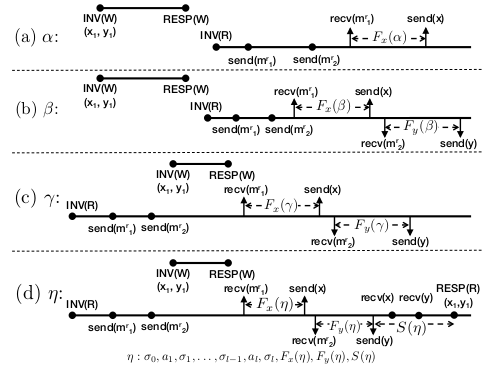
\includegraphics[scale=0.60]{figures/fig4.pdf} 
         %KMK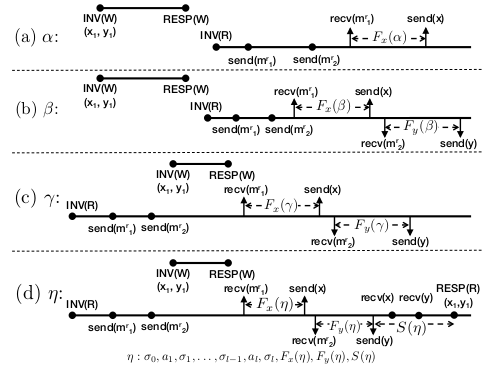
\includegraphics[width=4in]{figures/fig4.png} 
         \vspace{-2.0em}
         \caption{
\small{Schematic representation of executions $\alpha$, $\beta$, $\gamma$ and $\eta$,
          of ${\mathcal A}$ with transactions $R$ and $W$. The executions evolve from left to right. 
          The dots denote external events at clients. 
          The up-arrow marks denote external actions at $s_x$. The down-arrow marks denote external actions at $s_y$.}} \label{fig:execution1}
 \end{figure}

\begin{figure}[!ht]
      \centering
         %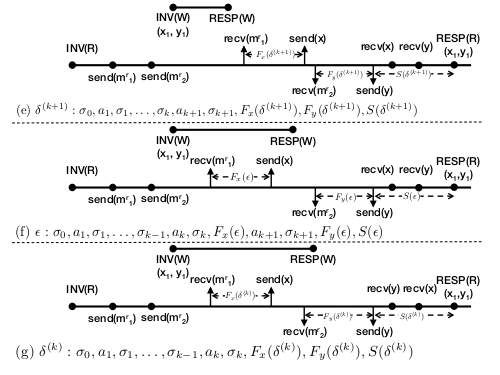
\includegraphics[width=1.00\textwidth]{figures/fig5.pdf} 
         %KMK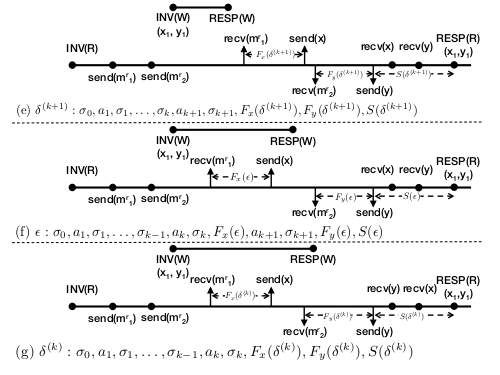
\includegraphics[width=4in]{figures/fig5.png}
         \vspace{-2.0em}
        \caption{\small{Executions $\delta^{(k+1)}$, $\epsilon$, and $\delta^{(k)}$, which show a progressive sequence of executions that are built on execution $\eta$ in Fig.~\ref{fig:execution1}.}}
         %\caption{\small{From execution $\eta$ of $\mathcal{A}$,  the construction of the progressive sequence of executions 
         %$\delta, \delta', \ldots$,  of  $\mathcal{A}$, of the form $\prefix{\cdot } \circ \frag{1,x}{\cdot}\circ \frag{1,y}{\cdot} \circ \suffix{\cdot}$. 
%The final execution $\phi$ of $\mathcal{A}$ to contradict the S property.}} 
      \label{fig:execution2}
\vspace{-1em}
 \end{figure}
}


\begin{figure*}[t]
	%\centering
	\hspace*{-0.7cm}
	\begin{subfigure}{0.49\textwidth}
		\centering
	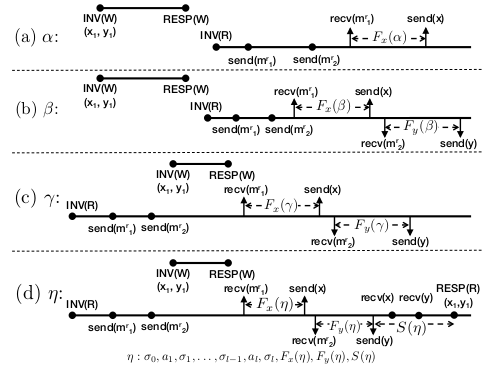
\includegraphics[width=1.2\linewidth]{figures/fig4.png}
	\end{subfigure}
	\hspace*{0.0m}  
	\begin{subfigure}{0.49\textwidth}
		\centering
	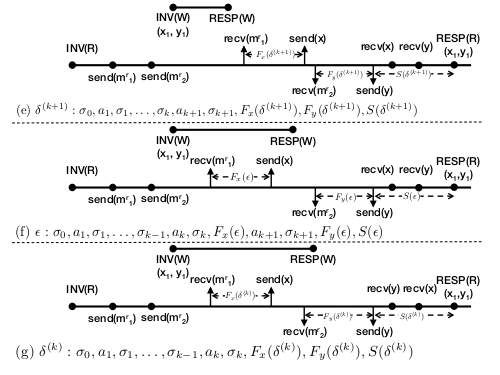
\includegraphics[width=1.2\linewidth]{figures/fig5.png}
	\end{subfigure} 
	         \caption{
	         	\small{Schematic representation of executions $\alpha$, $\beta$, $\gamma$ and $\eta$,
	         		of ${\mathcal A}$ with transactions $R$ and $W$. The executions evolve from left to right. 
	         		The dots denote external events at clients. 
	         		The up-arrow marks denote external actions at $s_x$. The down-arrow marks denote external actions at $s_y$.}} \label{fig:execution1}
\end{figure*}



\remove{
\begin{figure}[t]
\centering
\begin{subfigure}{1.0\columnwidth}
\centering
  \includegraphics[width=1.0\linewidth]{figures/fig4-1.pdf}
\end{subfigure}  
\begin{subfigure}{1.0\columnwidth}
\centering
  \includegraphics[width=1.0\linewidth]{figures/fig4-2.pdf}
\end{subfigure}  
\begin{subfigure}{1.0\columnwidth}
\centering
  \includegraphics[width=1.0\linewidth]{figures/fig4-3.pdf}
\end{subfigure}  


\caption{\small{try graphs}}
%% High level performance comparison between \eigermoon and Eiger with latency-throughput graph and comparisons on system overall throughput with varying degrees of skewness and write fractions.
%% Throughput comparison when varying system load and latency comparison of read-only transactions. Data staleness is measured by comparing \eigermoon to a linearizable baseline.}
\label{fig:latency}
\end{figure}
}


  The following proof proves Theorem~\ref{thm:two-snow}. In the proof we start with an execution $\eta$ and create a sequence of executions of 
  $\mathcal{A}$, where each one is of the form $\prefix{\cdot} \circ \frag{1,x}{\cdot}\circ \frag{1,y}{\cdot}\circ \suffix{\cdot}$, with progressively shorter $\prefix{\cdot}$ until we have a final execution that contradicts the $S$ property.
\remove{
 \begin{theorem}\label{thm:two-snow}
 The SNOW properties cannot be implemented in a system with two clients and two servers, where the clients do not communicate with each other.
\end{theorem}
}

\begin{proof}
\sloppy Consider an execution $\delta^{(\ell)}$  of $\mathcal{A}$ as in Lemma~\ref{lem:exec_delta}, and let $\prefix{\delta^{(\ell)}}$  be the execution fragment
$\finiteprefix{\ell-1}{\ell}$.
%, where $\ell$ is some positive integer, and $\sigma_i$'s and $a_i$'s denote states and actions, respectively. 
By  Lemma~\ref{lem:exec_delta}, $\RESP{R_1(\delta^{(\ell)})}$  returns
 $(x_1, y_1)$ and $\delta^{(\ell)}$ is also of the form    
$\finiteprefix{\ell-1}{\ell} \circ \frag{1,x}{\delta^{(\ell)}} \circ \frag{1,y}{\delta^{(\ell)}} \circ \suffix{\delta^{(\ell)}}$.     
%Below we will show that from $\delta$ we can create another execution $\delta^{(\ell-1)}$ of the form $\finiteprefix{\ell-2}{\ell-1} \circ \frag{1,x}{\delta^{(\ell-1)}} \circ \frag{1,y}{\delta^{(\ell-1)}} \circ \suffix{\delta^{(\ell-1)}}$ where   $\RESP{R(\delta^{(\ell-1)})}$  returns $(x_1, y_1)$. Note that $\prefix{\delta^{(\ell-1)}}$ ($\equiv  \finiteprefix{\ell-2}{\ell-1} $) is a prefix of $\prefix{\delta^{(\ell)}}$.

Next, we inductively prove the existence of a finite sequence of executions of $\mathcal{A}$---i.e., by proving the existence of a new execution based on the existence of a previous one---as $\delta^{(\ell)}, \delta^{(\ell-1)}, \cdots \delta^{(i)}, \delta^{(i-1)},  \cdots \delta^{(f)}$, 
for some positive integer $f$, with the following properties: $(a)$ Each of the execution in 
the sequence can be written in the form  $\finiteprefix{i-1}{i} \circ \frag{1,x}{\delta^{(i)}} \circ \frag{1,y}{\delta^{(i)}} \circ \suffix{\delta^{(i)}}$ (or $\prefix{\cdot}\circ \frag{1,x}{\cdot}\circ \frag{1,y}{\cdot}\circ\suffix{\cdot}$); $(b)$ for each $i$, $f \leq i  < \ell$, we have  $\prefix{\delta^{(i)}}$ to be a prefix of $\prefix{\delta^{(i+1)}}$; and $(c)$ $R_1(\delta^{(f)})$  returns  $(x_0, y_0)$, and for any $i$,  $f <  i \leq \ell$,  we have   $R_1(\delta^{(i)})$  that returns  $(x_1, y_1)$.  Note that there is a final execution of the form $\delta^{(f)}$  because of the initial values of $x_0$ and $y_0$  and the \wot{}  $W$. 

%and $(d)$  the $\frag{1,x}{\delta^{(f)}}\circ \frag{1,y}{\delta^{(f)}}$   occurs before $\INV{W}$ in $\delta^{(f)}$. 

%The claims $(a)$, $(b)$ and $(c)$ is due to Lemma~\ref{two:induction}, and $(d)$ follows from the fact that $\prefix{\delta^{(\ell)}}$ is a finite prefix.

%\end{proof}
 
%\begin{proof}
 %Consider  $\delta$ which is of the form 
%$\finiteprefix{k}{k +1} \circ \frag{1,x}{\delta} \circ \frag{1,y}{\delta} \circ \suffix{\delta}$, where   transaction 
%$R(\delta)$ responds with 
%$(x_1, y_1)$.
Clearly, there exists an integer $k$,  $ f \leq  k < \ell$, such that $\frage{R}{\delta^{(k)}}{}$ returns $(x_0, y_0)$ and $\frage{R_1}{\delta^{(k+1)}}{}$ returns $(x_1, y_1)$. Now we start with execution 
$\delta^{(k+1)}$ and construct an execution $\delta^{(k)}$ as described in the rest of the proof. The following argument will show that  $\frage{R}{\delta^{(k)}}{}$ must also return $(x_1, y_1)$, which contradicts the assumption of having the $S$ property.

Consider the execution $\delta^{(k+1)}$ of the form 
$\finiteprefix{k}{k +1} \circ \frag{1,x}{\delta^{(k+1)}} \circ \frag{1,y}{\delta^{(k+1)}} \circ \suffix{\delta^{(k+1)}}$. 
 The action  $a_{k+1}$ can  occur at any of the automata $r$, $w$, $s_x$, and $s_y$. Therefore, we consider the following four possible cases.
%

\emph{ \underline{Case (i) $a_{k+1}$ occurs at $w$:}} The execution fragments
 $\frag{1,x}{\delta^{(k+1)}}$ and $\frag{1,y}{\delta^{(k+1)}}$ do not contain any input action  at $s_x$ or $s_y$. $a_{k+1}$ does not occur at $s_x$ or $s_y$. 
 %Therefore, the action $a_{k+1}$ cannot have any impact on them. 
 Therefore,
 the asynchronous network can
  delay the occurrence of $a_{k+1}$ at $w$ to create the 
   finite execution   
$\finiteprefix{k-1}{k } \circ \frag{1,x}{\delta^{(k+1)}} \circ \frag{1,y}{\delta^{(k+1)}}$,  
 of. Also, there exists an execution $\delta^{(k)}$ that
 is an extension of the above finite execution, where $R_1$ completes in $\delta^{(k)}$.
%
  Clearly, $\delta^{(k)}$ can be written as  
 $\finiteprefix{k-1}{k } \circ \frag{1,x}{\delta^{(k)}} \circ \frag{1,y}{\delta^{(k)}} \circ \suffix{\delta^{(k)}}$, where $ \suffix{\delta^{(k)}}$ is the tail of the execution resulting from the extension. Moreover,  
  $\frag{1,x}{\delta^{(k+1)}}$   is indistinguishable  from   
  $\frag{1,x}{\delta^{(k)}}$ at $s_x$, i.e., 
      $\frag{1,x}{\delta^{(k+1)}} \stackrel{s_x}{\sim} \frag{1,x}{\delta^{(k)}}$. 
% \footnote{We drop the superscript $A$, such as $s_x$ to $s_x$,  from the symbol above $\sim$ for formatting reasons, when necessary.}
   Therefore, $send(x)_{s_x, r_1}$ has the same object value 
   $x$ in both fragments, which means $R_1$ returns $x_1$, and thus $R_1(\delta^{(k)})$ must return $(x_1, y_1)$ by the property $S$.
   % By the liveness property of a \rot{},  deduced from  O and N properties of the underlying read operations,  $R$ completes in $\delta'$.
   
   
\emph{ \underline{Case (ii) $a_{k+1}$ occurs at $r$:}} Similar to Case $(i)$.

\emph{ \underline{Case (iii) $a_{k+1}$ occurs at $s_x$:}} Observe that the two execution fragments  
   $a_{k+1} \sigma_{k+1} \circ \frag{1,x}{\delta^{(k+1)}}$ and $\frag{1,y}{\delta^{(k+1)}}$ occur at separate  automata, i.e., at $s_x$ and $s_y$ respectively. 
    Also, the  execution fragments  $a_{k+1} \sigma_{k+1} \circ \frag{1,x}{\delta^{(k+1)}}$ and $\frag{1,y}{\delta^{(k+1)}}$ do not contain any  input actions at $s_x$ or $s_y$. 
    Therefore, 
    %by Claim~\ref{claim:reorder}, 
    we can create an execution $\epsilon$, which  can be expressed as 
    $\finiteprefix{k-1}{k }  \circ \frag{1,y}{\epsilon}\circ a_{k+1}, \sigma_{k+1} \circ \frag{1,x}{\epsilon} \circ \suffix{\epsilon}$. Clearly,   
     $\frag{1,x}{\epsilon} \stackrel{s_x}{\sim} \frag{1,x}{\delta^{(k+1)}}$ and  
     $\frag{1,y}{\epsilon} \stackrel{s_y}{\sim} \frag{1,y}{\delta^{(k+1)}}$.  
     %
     %
     %$\suffix{\epsilon} \stackrel{s_y}{\sim} \suffix{\delta}$.
   %
%Below we argue that  we can create the execution $\epsilon$, of ${\mathcal A}$, where the two fragments are swapped with respect two their ordering in $\delta$. 
% If there are no output actions in the fragments then we can simply use the result Claim~\ref{claim:reorder} to swap 
 % the fragments in the execution to create the new  trace and from this,  by using Theorem~\ref{thm:trace} we create a new execution $\epsilon$. Otherwise,  in Theorem~\ref{thm:paste}  we consider sequence 
 % of actions $\beta$, as defined in the lemma,  where output actions corresponding to the fragments are swapped and then by the %result of the lemma      we realize  the existence of the execution $\epsilon$.
  Because $send(x)_{s_x, r_1}$ occurs in both $\frag{1,x}{\epsilon}$ and 
     $\frag{1,x}{\delta^{(k+1)}}$, it sends the same value $x_1$ to $r_1$. Therefore, $R$ returns $(x_1, y_1)$. 
   
   Now let us denote the execution fragment  $\finiteprefix{k-1}{k }  \circ \frag{1,y}{\epsilon}$ by $\epsilon'$, which  is simply a finite prefix of $\epsilon$.
     Allowed by the asynchronous network, we append $recv(m_x^{r_1})_{r_1, s_x}$ to $\epsilon'$, and create a finite execution $\epsilon''$ as 
        $\finiteprefix{k-1}{k }\circ \frag{1,y}{\epsilon''}, recv(m_x^{r_1})_{r_1, s_x}$, and delay any input action at $s_y$.    
        %Now, by Theorem~\ref{thm:extension} (1), there exists 
        
        Let $\epsilon'''$ be an extension of $\epsilon''$. Clearly,  
             $\frag{1,y}{\epsilon'''} \stackrel{s_y}{\sim} \frag{1,y}{\epsilon''}$, and thus $send(y )_{s_y, r_1}$ sends the same value $y_1$ in $\epsilon''$ and $\epsilon'''$. 
             By the $N$ property, $send(x)_{s_x, r_1}$ eventually occurs, and by the $O$ property $x$ is send to $r_1$. Therefore, $R_1$ completes in 
$\epsilon'''$, which implies that 
             $R(\epsilon''')$ must return $(x_1, y_1)$.
             
             Note that the execution fragment of $\epsilon'''$ has no input actions of $s_x$ between $ recv(m_x^{r_1})_{r_1, s_x}$ and $send(x)_{s_x, r_1}$, which can be identified as $\frag{1,x}{\epsilon'''}$. Therefore, $\epsilon'''$ can be written as      $\finiteprefix{k-1}{k }  \circ \frag{1,y}{\epsilon'''} \circ \frag{1,x}{\epsilon'''} \circ \suffix{\epsilon'''}$.
   
    Next, since $\frag{1,x}{\epsilon'''}$ and $\frag{1,y}{\epsilon'''}$ contain actions of different automata, 
    %by  Claim~\ref{claim:reorder},  
    we can create an execution prefix  $\epsilon^{(iv)}$ as 
    $\finiteprefix{k-1}{k }  \circ \frag{1,x}{\epsilon^{(iv)}} \circ \frag{1,y}{\epsilon^{(iv)}}$, 
     where  
     $\frag{1,x}{\epsilon^{(iv)}}$ appears before $\frag{1,y}{\epsilon^{(iv)}}$. Next, 
     % by using Theorem~\ref{thm:extension} $(1)$ 
     we create an execution $\delta^{(k)}$ as an extension of 
       $\epsilon^{(iv)}$, which can be written   as $\finiteprefix{k-1}{k } \circ \frag{1,x}{\delta^{(k)}} \circ \frag{1,y}{\delta^{(k)}}\circ \suffix{\delta^{(k)}}$. 
       Then by the $O$ and $N$ properties, $R_1$ completes in $\delta^{(k)}$.  
       Since $\frag{1,x}{\epsilon^{(iv)}} \stackrel{s_x}{\sim} \frag{1,x}{\epsilon'''}$, $send(x)_{s_x, r_1}$ returns $x_1$ in $\epsilon^{(iv)}$. 
    Similarly, because 
      $\frag{1,x}{\delta^{(k)}} \stackrel{s_x}{\sim} \frag{1,x}{\epsilon^{(iv)}}$, $send(x)_{s_x, r_1}$ returns $x_1$ in $\delta^{(k)}$. So,
     $R_1(\delta^{(k)})$ returns $(x_1, y_1)$.
  %

\emph{ \underline{Case (iv) $a_{k+1}$ occurs at $s_y$:}} Because $a_{k+1}$ occurs at server $s_y$ and $\frag{1,x}{\delta^{(k+1)}}$ occurs at server $s_x$ (different automata),  
%then by applying  Claim~\ref{claim:reorder}  as in the previous cases 
we can create a new execution $\epsilon$ of $\mathcal{A}$ (Fig.~\ref{fig:execution2} $(f)$)  as   
             $\finiteprefix{k-1}{k } \circ \frag{1,x}{\epsilon} \circ a_{k+1}, \sigma_{k+1} \circ 
        \frag{1,y}{\epsilon}\circ \suffix{\epsilon}$, such that $\frag{1,x}{\epsilon} \stackrel{s_x}{\sim}\frag{1,x}{\delta^{(k+1)}}$, where  
         $a_{k+1}, \sigma_{k+1} $
       occurs after $\frag{1,x}{\delta^{(k+1)}}$ and 
         $R(\epsilon)$ returns $(x_1, y_1)$.
        
     Now, consider the finite execution   $\finiteprefix{k-1}{k }\circ \frag{1,x}{\epsilon}$ at the end of which we append $recv(m_y^{r_1})_{r_1, s_y}$ to create a finite execution of $\mathcal{A}$ as 
        $\finiteprefix{k-1}{k }\circ \frag{1,x}{\epsilon}, recv(m_y^{r_1})_{r_1, s_y}$. 
        %Now, by Theorem~\ref{thm:extension} (1), 
        Then, there exists 
        an execution $\epsilon'$ of $\mathcal{A}$, where 
              the network delays the input actions at $s_y$. By the $N$ and $O$ properties, $send(y)_{s_y, r_1}$ occurs in $\epsilon'$. Clearly, since   $\frag{1,x}{\epsilon'} \stackrel{s_x}{\sim} \frag{1,x}{\epsilon}$, $send(x)_{s_x, r_1}$ sends the same value in $\epsilon$ and $\epsilon'$. Therefore,  $R_1$ returns $(x_1, y)$.
              
              In $\epsilon'$, we denote the fragment that begins with $recv(m_y^{r_1})_{r_1, s_y}$ and ends with 
              $send(y)_{s_y, r_1}$ by $\frag{1,y}{\epsilon'}$ to have $\epsilon'$ as  
              $\finiteprefix{k-1}{k } \circ \frag{1,x}{\epsilon'}  \circ 
        \frag{1,y}{\epsilon'}$. 
        %Now using Theorem~\ref{thm:extension} (1), we know 
        Then, there exists 
        an execution $\delta^{(k)}$ of $\mathcal{A}$, which is an extension of $\epsilon'$. Clearly, $\delta^{(k)}$ can be written as 
     $\finiteprefix{k-1}{k }  \circ \frag{1,x}{\delta^{(k)}} \circ \frag{1,y}{\delta^{(k)}} \circ \suffix{\delta^{(k)}}$, where $\suffix{\delta^{(k)}}$ is the tail of the extended execution.  Clearly,  $\frag{1,x}{\delta^{(k)}} \stackrel{s_x}{\sim} \frag{1,x}{\epsilon'}$. Therefore,  $R_1(\delta^{(k)})$ returns $x_1$ in $\delta^{(k)}$, which implies $R_1(\delta^{(k)})$ must return $(x_1, y_1)$.    
\end{proof}

\remove{
 
 \begin{figure}[!ht]
      \centering
         %kmk\includegraphics[width=0.50\textwidth]{figures/architecture3_1.png}  \vspace{-2.5em}
         \caption{
\small{The architecture of a typical web service with clients, servers, and 
         % The external requests and responses  at the clients  to and from the end-users are represented as invocation and responses for the transaction.
         the communication channels, between every pair of processes, inside a datacenter is modeled as a collection of I/O automata. Note that, unlike the architecture in Fig.~\ref{fig:architecture2a}, in this setup there are communication channels between every pair of clients.}} 
         \label{fig:architecture2c}
 \end{figure}

}

%\section{SNOW on MWSR with client-to-client messages} \label{mwsr}

\subsection{SNOW with C2C Communication}
 \label{subsec:yes_snow_yes_c2c}
\label{sec:mwsr}
In this section, we state that  SNOW is possible in the   \emph{multiple-writers single-reader} 
(MWSR) setting %, and prove that any fair and well-formed execution  of $A$ satisfies  the SNOW properties.  
%In practice, a system with a single reader may not be very useful but this algorithm serves a counter example 
%algorithm
 when client-to-client communication is allowed.  
%Algorithm $A$ 
%shows that if client-to-client communication is allowed, it is possible to have algorithms  that satisfies all of the SNOW properties with two clients. 
We consider a system that has $\ell \geq 1$ writers with ids $w_1, 
w_2 \cdots w_{\ell} \in \mathcal{W}$ 
%(we denote this set by $\mathcal{W}$)
, one reader $r$, and  $k \geq 1$ servers with ids $s_1, s_2\cdots s_k \in \mathcal{S}$. 
%(denote as $\mathcal{S}$) that maintains the  objects $o_1, \cdots, o_k$, respectively. 
Client-to-client communication is allowed. 
%Note that for a two-client system, when both  clients are of the same type, i.e., two writers or two readers, the SNOW properties are trivially satisfied.
	%			
% For any two tags $t_1, t_2 \in \mathcal{T}$ we say  $t_2 > t_1$ if $(i)$ $t_2.z > t_1.z$ or $(ii)$ $t_2.z = t_1.z$ and $t_2.w > t_1.w$. Therefore, the set $\mathcal{T}$ is totally ordered set. We also assume that every client and servers has a unique id and the ids can be compared w.r.t. some lexicographic order.
%
The following theorem states that in such a setting  it is possible to have an algorithm  that respects all SNOW properties.  Due to space constraints, we do not present the algorithm or the proof for the theorem, {\color{blue} which can be found in the extended version of the paper.} %, where \wots{} are live. % and the proof is omitted, for now, since it is very straightforward. 


%Consider any failure-free execution of algorithm $A$. In the steps for the reader assume the quantity
 %$t_r \triangleq \max_{1 \leq j \leq |List|} \{ j : List[j].b_i = 1 \wedge i \in I\}$, which is presented as a comment in the pseudo-code for $A$.
%We associate with any transaction $\phi$ a tag
%$tag(\phi)$ such that if  $\phi$ is a \wot{}  $tag(\phi)=t_w$, i.e., the value of $t_w$ before the completion of the operation, and $tag(\phi)=t_r$ when $\phi$ is a \rot{}.
		
\begin{theorem} In the MWSR setting, there exists an algorithm $A$ such that
	any  well-formed  and fair execution of $A$  implements a wait-free  transaction processing system, $T$, for objects of type $\mathcal{O}_T$, consisting of  objects $o_1, o_2, \cdots o_k$ at servers $s_1, s_2, \cdots, s_k$, respectively; and $T$ respects the SNOW properties and \wots{} are live.
\end{theorem}
	
\remove{
	\begin{proof} Below we show that $A$ satisfies the  SNOW properties. 
	
	\noindent{\emph{\underline{S property:}}} 
	Let $\beta$ be any fair execution  of  $A$ and 
 suppose all clients in $\beta$ behave in a well-formed
manner. Suppose $\beta$ contains no incomplete transactions and let  $\Pi$ be the set of transactions in $\beta$.  We define an irreflexive partial ordering ($\prec$) among the transactions in $\Pi$ as follows:  if $\phi$ and $\pi$ are any two distinct transactions in $\Pi$ then we say 
	$\phi \prec \pi$ if either $(i)$ $tag(\phi) < tag(\pi)$ or $(ii)$ $tag(\phi) = tag(\pi)$ and $\phi$ is a \wot{} and $\pi$ is a \rot{}. We will prove the $S$  (strict-serializability) property of $A$ by proving that the properties $P1$, $P2$, $P3$ and $P4$ of Lemma~\ref{lem:equivalence} hold for $\beta$. 
	
	\emph{P1:}   If $\pi$ is a \rot{} then since all \rots{} are invoked by a single reader $r$ and in a well-formed manner, 
	therefore, there cannot be an infinite number of \rots{} such that they all 
	precede $\pi$ (w.r.t $\prec$).
	 Now, suppose $\pi$ is a \wot{}. Clearly, from an inspection of the algorithm, 
	 $tag(\pi) \in \mathbb{N}$. From inspection of the algorithm, each \wot{} increases the size of 
	 $List$, and the value of the tags are  defined by the size of $List$. Therefore, there can be at 
	 most a finite number of \wots{} such that can precede $\pi$ (w.r.t. $\prec$) in $\beta$.
	  
	\emph{P2:}  Suppose $\phi$ and $ \pi$ are any two transactions in $\Pi$, such that, $\pi$ begins after $\phi$ completes. 
	Then we show that we cannot have $\pi \prec \phi$. Now, we consider four cases, depending on whether $\phi$ and $\pi$ are \rots{} or \wots{}.	
	\begin{enumerate}
	    \item [$(a)$] $\phi$ and $\pi$ are \wots{} invoked by writers $w_{\phi}$ and $w_{\pi}$, respectively. Since the size of $List$, in $r$,  grows monotonically with each \wot{}  hence  $w_{\pi}$ receives the  tag at least as high as $tag(\phi)$, so $\pi\not \prec \phi$.
	      %
	       \item [$(b)$] $\phi$ is a \wot{}, $\pi$ is a \rots{} invoked by writer $w_{\phi}$ and $r$, respectively.  
	        Since the size of $List$, in $r$,  grows monotonically, and because  $w_{\pi}$ invokes $\pi$ after $\phi$ completes hence  $tag(\pi)$ is at least as high as $tag(\phi)$, so $\pi\not \prec \phi$.
	      %
	        \item[$(c)$] $\phi$ and $\pi$ are \rots{}  invoked by reader $r$. 
	           Since the size of $List$, in $r$,  grows monotonically,  hence  $w_{\pi}$ invoked $\pi$ after $\phi$ completes hence $tag(\pi)$ is at least as high as $tag(\phi)$, so $\pi\not \prec \phi$.
	        %
	         \item [$(d)$] $\phi$ is a \rot{}, $\pi$ is a \wot{}  invoked by reader $r$ and $w_{\pi}$, respectively.
	         This case is simple because new values are added to $List$  only  by writers, and $tag(\pi)$ 
	         is larger than the tag of $\phi$ and hence   $\pi\not \prec \phi$. 
	\end{enumerate}
	
	\emph{P3:} This is clear by the fact that any \wot{} always creates a unique tag and all tags are totally ordered since they all belong to $\mathbb{N}$
	
	\emph{P4:} Consider a \rot{} $\rho$ as $READ(o_{i_1}, o_{i_2}, \cdots, o_{i_q})$, in $\beta$. 
Let the returned value from $\rho$ be $\mathbf{v} \equiv $$(v_{i_1}, v_{i_2}, \cdots, v_{i_q})$ such that 
$1 \leq {i_1} <  {i_2} <  \cdots <  {i_q} \leq k$, where value  $v_{i_j}$ corresponds to $o_{i_j}$. 
	Suppose $tag(\rho) \in \mathbb{N}$ was created during some \wot{}, say $\phi$, i.e., $\phi$ is the \wot{} that 
	added the elements in index $(tag(\rho)-1)$ of $List$. Note that element in index $0$ contains the initial value.
	%because \rots{} do not generate new tags as they do not add any new item to the $Vals$ of any server.
	 Now we consider two cases:
	 
	\emph{Case $tag(\rho) = 1$.} We  know that it corresponds the initial default value $v_i^0$ at each sub-object $o_i$, and this equates to $\rho$ returning the default initial value for each sub-object.
	 %
	% Therefore, $tag(\rho) = tag(\phi)$. 
	 
	 \emph{Case $tag(\rho) > 1$.} Then we argue that there exists no \wot{}, say $\pi$, that updated object $o_{i_j}$,   in $\beta$, such that,  $\pi \neq \phi$ and $\rho$ returns values written by $\pi$ and $\phi \prec \pi \prec \rho$. Suppose we assume the 	contrary, which means $tag(\phi) < tag(\pi) < tag(\rho)$. The latter implies $tag(\phi)  = tag(\pi)$ which is not possible because 
	this contradicts the fact that for any two distinct \wots{} $tag(\phi) \neq tag(\pi)$  in any execution of   $A$.
	
	\noindent{\emph{\underline{N property:}}}  By inspection of algorithm $A$ for the  response steps  of the servers to the reader.
	
	\noindent{\emph{\underline{O property:}}} By inspection of the  {\readValue} phase: it consists of one round of communication between the reader and the servers, where the servers send only one version of the value of the object it maintains.
	
	\noindent{\emph{\underline{W property:}}}  By inspection of the \wot{} steps, and  and  that writers always get to complete the transactions they invoke.
	%Finally, the liveness property of \wots{} can be realized by inspecting the steps of  algorithm $A$.
	\end{proof}
}

 %Note that the above theorem still holds even if any writer crashes.



\remove{
\section{Bounded Latency}
\subsection{No Prior Bounded Latency for SW}\label{sec:eiger}
%The original SNOW work claimed that after examining existing work there existed one system, Eiger~\cite{Lloyd:nsdi2013}, whose \rots{} had bounded latency---i.e., non-blocking and finish in three rounds---while providing the strongest guarantees--i.e., having properties W and S---because Eiger claimed that its \rots{} provide strict serializability within a datacenter, even if providing strict serializability was not a focus of Eiger. 

In this section, we correct this claim and show there were no existing algorithms that had bounded latency while providing the strongest guarantees by proving Eiger's \rots{} are not strictly serializable. The insight is that Eiger uses logical timestamps to track the ordering of operations while logical clocks are not able to enforce the real-time ordering between operations. Strict serializability, however, requires the real-time ordering to be respected. For details of the proof, please see Appendix~\ref{app:eiger_not_s}.

In the following subsections, we provide the first set of novel algorithms that have bounded latency and  strongest guarantees.


\vspace{-1em}
\subsection{SNW +  One Version,  MWMR setting}\label{mwmr_snow_one_version}
%%\section{SNoW for MWMR setting}\label{mwmr}
Here present  algorithm  $B$, which satisfies  SNW and "one-version" properties, in MWMR setting where a \rot{} must consist of one version of the data but, possibly, multiple communication trips between the reader and the servers.% We denote the type of object  that satisfies the SNoW properties by $\tilde{\mathcal{O}}_T$.   
%Note that $B$ can also tolerate crash failure of writers and readers. 
In B, the steps for the writers are shown in Pseudocode~\ref{fig:algo_bc} and for readers and the servers  are presented in Pseudocode~\ref{fig:algo_b}.
We assume  a set of writers $\mathcal{W}$,  a set of readers $\mathcal{R}$ and a set of $k \geq 1$ servers,  $\mathcal{S}$, with ids $s_1, s_2\cdots s_k$ that stores the objects $o_1, o_2, \cdots, o_k$, respectively.  We define  key ${\kappa}$ is defined as a pair $(z, w)$, 
where $z \in \mathbb{N}$ and $w \in \mathcal{W}$ the  id of a writer. We use $\mathcal{K}$ to denote the set of all possible keys. 
In $B$, the keys are used to uniquely identify each transaction. Also, with each transaction we associate a tag $t \in \mathbb{N}$. 
%We assume writers can send message to the reader, i.e., we allow client-to-client messages.
% We assume that each process has a unique id. We assume that each server $s$ stores object $o_s$, due to sharding.  For the sake of simplicity, we assume that the \wots{} issued by a writer are of the form: \emph{ write value $v_1$ to object $o_1$, $v_2$ to $o_2$, and so on}. In other words, we assume that such a  transaction consists of the set of operations $\{ \writeop{o_1}{v^{(1)}}, \writeop{o_2}{v^{(2)}}\cdots \writeop{o_k}{v^{(k)}}\} $, which we denote by $write(v_1, v_2, \cdots, v_k)$.  \wots{} where only a subset of  the objects are updates will be discussed later. We also assume that  the \rots{} are of the form  $\{ \readop{o_1}, \readop{o_2}\cdots \readop{o_k}\}$ consisting of $k$ reads to $k$ distinct objects.	
	
In  $B$, we designate one of the servers as coordinator, denote as $s^*$,
 for the transactions. The $s^*$  maintains the order of the \wots{} and the objects that are updated during the \wot{} in the variable $List$.  %Note that in a system, where there are many objects 
%different objects may be use different servers  as coordinators based on some load-balancing rule. 

\textit{\textbf{State variables:}} Each of the writers and servers maintain a set of state variables as follows: $(i)$ At  any  \emph{writer $w$}, there is  a counter $z$ to keep track of the
 number of \wot{}  the writer has  invoked, initially $0$. $(ii)$ At any  \emph{server}, $s_i$, 
 for $i \in [k]$, there is  a set variable $Vals$ 
 with elements 
 that are  key-value pairs $({\kappa}, v_i) \in \mathcal{K} \times \mathcal{V}_i$. Initially,
  $Vals= \{ ({\kappa}^0, v_i^0)\}$. %This ensures that each \wot{} generates a unique key.
A server also contains an
 ordered list variable $List$  of elements  as $({\kappa}, (b_1, \cdots, b_k))$,  where 
 ${\kappa}  \in \mathcal{K}$  and 
 $(b_1, \cdots b_k) \in  \{0, 1\}^k$. Initially,  
 $List= [ ({\kappa}^0, (1, \cdots 1) ]$, where ${\kappa}^0  \equiv (0, w_0)$, 
 where $w_0$ is any
  place holder identifier string for writer id. The elements in $List$ can be identified with an index, e.g., 
  $List[0] =({\kappa}^0, (1, \cdots, 1))$.  Essentially, a $(k+1)$-tuple  $(\kappa, (b_1, \cdots, b_k))$ in $List$ corresponds to a \wot{} and 
   identifies the set of objects that are updated during the \wot{}, i.e., if $b_i=1$ then object 
   $o_i$ was updated  during  the  \wot{}, otherwise $b_i=0$.
			%labeled with phase names, viz., {\readGetTag}, {\readValueTag}, {\readCompleteTag} and {\writeGetTag}. The server to server messages are labeled as {\readDisperseTag}. Also, in some phases of {\SODA},  the message-disperse primitives {\mdmetaprim} and {\mdvalueprim} are used  as services. 
					
\textit{\textbf{Writer steps:}} A \wot{} updates
			a  list of $p$ objects $o_{i_1}, o_{i_2}, \cdots o_{i_p}$  with values
			 $v_{i_1}, v_{i_2}, \cdots v_{i_p}$, respectively, is invoked at $w$ via the procedure
			$\Writetr{ (o_{i_1}, v_{i_1}), \cdots, (o_{i_p}, v_{i_p}) }$.
We use the notations:  $I \triangleq \{i_1, i_2, \cdots, i_p\}$  and $S_I\triangleq \{s_{i_1}, s_{i_2}, \cdots, s_{i_p}\}$.
This procedure  consists of two phases: {\writeValue} and {\updateCoord}. 
%We denote the set of servers involved   in the \wot{}  by  $S_I=\{s_{i_1}, s_{i_2}, \cdots, s_{i_p}\}$.   
During the {\writeValue} phase,  $w$ creates a new key ${\kappa}$ as 
 $ {\kappa}  \equiv (z + 1, w)$, where $w$ identifies the writer; and also increments the local counter $z$ by one.  Then $w$ sends $(${\writeValueTag}$, ({\kappa}, v_{i}))$ to each server in $S_I$, and awaits {\ackTag}  
from all servers in $S_I$.
After receiving {\ackTag} from all servers in $S_I$,  $w$
initiates the {\updateCoord} phase where it sends 
(\updateCoordTag, $({\kappa}, (b_{1}, \cdots b_{k})$) to $s^*$, where for any $i \in [k]$,  $b_i=1$ if $s_i \in S_I$, 
otherwise $b_i=0$,   and completes then \wot{} after it receive a   ({\ackTag}, $t_w$) from $s^*$.  
%	  After receiving message  ({\ackTag}, $t_w$),  $w$ completes the \wot{}.

%At $s^*$, upon receiving  (\updateCoordTag, $({\kappa}, (b_{1}, \cdots, b_{k})$) from $w$ appends  
%			 $({\kappa}, (b_{1}, \cdots, b_{k}))$ to its  $List$,  and responds with  
%			 {\ackTag} and $t_{w}$ (set to be the number of elements in the local list $List$)  to $w$.
%			 The order of the  elements in  $List$ corresponds to  the order  
%the \wots{}, the order of the incoming  {\updateCoordTag} updates,  as seen by $s^*$.
%			  After receiving an ({\ackTag}, $t_w$),  $w$ completes the \wot{}.

\textit{\textbf{Reader steps:}}
We use the same notations for $I$ and $S_I$ as above but the indices can vary across  transactions.
The procedure  \Readtr{$ o_{i_1},  o_{i_2}, \cdots, o_{i_p}$} can be 
initiated by  some reader  $r$,   as a \rot{}, intending to read the values of 
subset $o_{i_1},  o_{i_2}, \cdots, o_{i_p}$ of the objects. The procedure 
consists of two consecutively executed phases of communication rounds
between the $r$ and the  servers, viz.,  {\getTagArray} and {\readValue}. 
%
During  the  phase {\getTagArray},  $r$ sends $s^*$ the message  {\getTagArrayTag}  
 requesting the  list of the latest added keys for each object. 
 Once $r$ receives a list of tags, such as, $(t_r, ({\kappa}_1, {\kappa}_2, \cdots,  {\kappa}_k))$ from $s^*$   the phase completes.
%
%
In the subsequence phase, {\readValue},   $r$ requests each server $s_i$ in $S_I$ by sending the message 
$(\text{\readValueTag}, \kappa_i)$. 
% Then upon receiving such a request, any server $s_i$ responds with  $(${\readValueTag}$, {\kappa}^{s_i})$, i.e., one version of  $o_i$ corresponding to the key $t_i$ to $r$, stored in its $Vals$. 
%
%During  phase {\readValue}, 	 the reader sends to each of the servers in 
%$\mathcal{S}$, say $s_i$ the key ${\kappa}^{s_i}$ corresponding 
%			 to $(k+1)$-tuple of $List$ with the latest  index $j^*$ such that $b_i =1$ such that 
%$i \in I$, where $I \triangleq  \{{i_1},  {i_2}, \cdots, {i_p}\}$,  requesting the corresponding value.  
%Any server $s_i$ upon receiving 
%such a message with $(${\readValueTag}$, {\kappa}^{s_i})$ responds with $v$ such that $({\kappa}^{s_i}, v_i)$ is in its variable $Vals$. 
After  receiving the values $v_{i_1}$, $v_{i_2}, \cdots v_{i_p}$ from the servers in $\mathcal{S_I}$, 
 $r$ completes the transaction  by 
 returning the tuple of values $(v_{i_1}, \cdots v_{i_p})$.
 % and set the tag $t_r$ as  the latest index in $List$ corresponding to a \wot{} that updated  one of the object in the \rot{}, i.e., $\max_{1 \leq j \leq |List|} \{ j : List[j].b_i = 1 \wedge i \in I\}$.

\textit{\textbf{Server steps:}}  
When a server $s_i$ receives a message of type $(${\writeValueTag}$, ({\kappa}, v_{i}))$ from a writer $w$ then 
%to each server in $S_I$, and awaits {\ackTag}  
%from all servers in $S_I$.
it  adds $({\kappa}, v_i)$ to its set variable  
$Vals$ and sends {\ackTag} back to $w$.

If the coordinator $s^*$ receives  (\updateCoordTag, $({\kappa}, (b_{1}, \cdots, b_{k})$) from writer $w$, then it appends  
			 $({\kappa}, (b_{1}, \cdots, b_{k}))$ to its  $List$,  and responds with  
			 {\ackTag} and $t_{w}$ (set to be the number of elements in the local list $List$)  to $w$.
			 The order of the  elements in  $List$ corresponds to  the order  
the \wots{}, the order of the incoming  {\updateCoordTag} updates,  as seen by $s^*$.
	
When $s^*$  receives  the message  {\getTagArrayTag} from $r$  it responds with 
$(\kappa_1, \cdots, \kappa_k)$ such that for each $i \in [k]$, $\kappa_i$ is the key  part of the $(k+1)$-tuple that was modified
last, i.e., 	${\kappa}_i = List[j^*].{\kappa}$ such that 	 $j^* \triangleq\max \{ j : List[j].b_i =1 \}$, and 
$t_r$, $t_r \triangleq \max_{1 \leq j \leq |List|} \{ j : List[j].b_i = 1 \wedge i \in I\}$.
%
  	If any server $s_i$ receives a message  $(${\readValueTag}$, {\kappa})$ from a reader $r$ then it responds to $r$ with 
   the value $v_i$ corresponding to key with value  $\kappa$ in  $Vals$. 

The following result states that algorithm $B$ respects SNW and "one-round" properties.
% and the proof is omitted for now since it is very straightforward. Note that the liveness property of \rot{} and \wot{}  transactions are a part of the SNOW properties.
%Consider any failure-free and fair execution of algorithm $B$. 
%For the purpose of proving the $S$ property, for every transaction transaction  $\phi$ in an execution of $B$ we associate a tag $tag(\phi)$ as described below.
% the variable $t_r$ in a reader and $t_w$ in 
%a writer are used to associate a tag as described below.
% $ \triangleq \max_{1 \leq j \leq |List|} \{ j : List[j].b_i = 1 \wedge i \in I\}$, which is presented as a comment in the pseudo-code for $A$.
%If $\phi$ is a \wot{} (\rot{}) then  $tag(\phi)$ is the value of the variable $t_w$ ($t_r$) immediately before the 
%operation completes.

\begin{theorem} Any well-formed  and fair execution of algorithm $B$  satisfies the SNW and "one-round"  properties. %Algorithm $B$ also tolerates any client crash failures.
\end{theorem}

%	\begin{theorem} Any well-formed  and fair execution of algorithm $B$ is an implementation of  an object of type $\tilde{\mathcal{O}}_T$ in the MWMR setting, 	with no client-to-client communication,  comprising of objects $o_1, o_2, \cdots o_k$ stored in servers $s_1, s_2, \cdots, s_k$, respectively; and it satisfies the SNoW  properties. %Algorithm $B$ also tolerates any client crash failures.\end{theorem}



\remove{
\begin{proof} Below we show that algorithm $B$ satisfies the  SNoW properties. 
	
	\noindent{\emph{\underline{S property:}}} 
	Let $\beta$ be any fair execution  of  $B$ and 
 suppose all clients in $\beta$ behave in a well-formed
manner. Suppose $\beta$ contains no incomplete transactions and let  $\Pi$ be the set of transactions in $\beta$.  We define an irreflexive partial ordering ($\prec$) in $\Pi$ as follows:  if $\phi$ and $\pi$ are any two distinct transactions in $\Pi$ then we say 
	$\phi \prec \pi$ if either $(i)$ $tag(\phi) < tag(\pi)$ or $(ii)$ $tag(\phi) = tag(\pi)$ and $\phi$ is a \wot{} and $\pi$ is a \rot{}. Below we prove the $S$  property of $B$ by showing that  properties $P1$, $P2$, $P3$ and $P4$ of Lemma~\ref{lem:equivalence} hold for $\beta$. 
	
	\emph{P1:}   Clearly, from an inspection of the algorithm, 
	 $tag(\pi) \in \mathbb{N}$. From inspection of the algorithm, each \wot{} increases the size of 
	 $List$, and the value of the tags are  defined by the size of $List$. Therefore, there can be at 
	 most a finite number of \wots{} such that can precede $\pi$ (w.r.t. $\prec$) in $\beta$.
	  On the other hand, if $\pi$ is a \rot{} then since all \rot{}s are invoked by readers  in a well-formed manner,  and there are only finite number of readers 
	therefore, there cannot be an infinite number of \rot{}s such that they all 
	precede $\pi$ (w.r.t $\prec$).
	
	 
	  
	\emph{P2:}  Suppose $\phi$ and $ \pi$ are any two transactions in $\Pi$, such that, $\pi$ begins after $\phi$ completes. Then we show that we have  we cannot have $\pi \prec \phi$. Now, we consider four cases, depending on whether $\phi$ and $\pi$ are \rot{}s or \wots{}.	
	\begin{enumerate}
	    \item [$(a)$] $\pi$ and $\phi$ are \wots{} invoked by writers $w_{\pi}$ and $w_{\phi}$, respectively. Since the size of $List$, in $s^*$ grows monotonically due to each \wot{}  hence  $w_{\pi}$ receives the  tag  from $s^*$ at least as high as $tag(\phi)$, so $\pi\not \prec \phi$.
	      %
	       \item [$(b)$] $\pi$ is a \rot{}, $\phi$ is a \wot{} invoked by reader  $r_{\pi}$ and writer $w_{\phi}$, respectively.  
	        Since the size of $List$, in $s^*$,  grows monotonically,  because  $r_{\pi}$  invokes $\pi$ after $\phi$ completes hence $tag(\pi)$ is at least as high as $tag(\phi)$, so $\pi\not \prec \phi$.
	      %
	        \item[$(c)$]$\pi$ and $\phi$ are both \rot{}s  invoked by readers $r_{\pi}$ and $r_{\phi}$, respectively. 
	           Since the size of $List$, in $s^*$, grows monotonically,  because   $w_{\pi}$ invokes $\pi$ after $\phi$ completes hence $tag(\pi)$ is at least as high as $tag(\phi)$, so $\pi\not \prec \phi$.
	        %
	         \item [$(d)$] $\pi$ is a \wot{}, $\phi$ is a \rot{}  invoked by writer $w_{\pi}$ and reader $r_{\phi}$, respectively.
	         This case is simple because new values are added to $List$, in $s^*$,  only  by writers, and $tag(\pi)$  has to be larger than the tag of $\phi$ and hence   $\pi\not \prec \phi$. 
	\end{enumerate}
	
	
	\emph{P3:} This is from  the fact that any \wot{} always creates a unique tag and all tags are totally ordered since they all belong to $\mathbb{N}$
	
		\emph{P4:} Consider a \rot{} $\rho$ as $READ(o_{i_1}, o_{i_2}, \cdots, o_{i_q})$, in $\beta$. 
Let the returned value from $\rho$ be $\mathbf{v} \equiv $$(v_{i_1}, v_{i_2}, \cdots, v_{i_q})$ such that 
$1 \leq {i_1} <  {i_2} <  \cdots <  {i_q} \leq k$, where value  $v_{i_j}$ corresponds to $o_{i_j}$. 
	Suppose $tag(\rho) \in \mathbb{N}$ was created during some \wot{}, say $\phi$, i.e., $\phi$ is the \wot{} that 
	added the elements in index $(tag(\rho)-1)$ of $List$ at the coordinator $s^*$. Note that element in index $0$ contains the initial value.
	%because \rots{} do not generate new tags as they do not add any new item to the $Vals$ of any server.
	 Now we consider two cases:
	 
	\emph{Case $tag(\rho) = 1$.} We  know that it corresponds the initial default value $v_i^0$ at each sub-object $o_i$, and this equates to $\rho$ returning the default initial value for each sub-object.
	 %
	% Therefore, $tag(\rho) = tag(\phi)$. 
	 
	 \emph{Case $tag(\rho) > 1$.} Then we argue that there exists no \wot{}, say $\pi$, that updated object $o_{i_j}$,   in $\beta$, such that,  $\pi \neq \phi$ and $\rho$ returns values written by $\pi$ and $\phi \prec \pi \prec \rho$. Suppose we assume the 	contrary, which means $tag(\phi) < tag(\pi) < tag(\rho)$. The latter implies $tag(\phi)  = tag(\pi)$ which is not possible because 
	this contradicts the fact that for any two distinct \wots{} $tag(\phi) \neq tag(\pi)$  in any execution of   $B$.

	\noindent{\emph{\underline{N, o and W properties:}}}  Evident from an inspection of the algorithm.
	% for the  response steps  of the servers to the reader.
	\end{proof}
}
%
\subsection{SNW + One Round,  MWMR setting}\label{mwmr_snow_one_round}
%%\section{\text{SN$\bar{o}$W} for MWMR setting}\label{mwmr_snow}
Here, we present  algorithm  $C$ which satisfies  SNW and "one-round"  properties in the MWMR setting, where a \textit{READ} consists one round of communications between the reader and the servers but servers may respond with multiple versions of the data. %We denote the type of object that satisfies the SN$\bar{o}$W properties by $\bar{\mathcal{O}}_T$.   
%Note that $B$ can also tolerate crash failure of writers and readers. 
The notation for the  writers, servers and tag are similar to algorithm $B$. 
Pseudocodes~\ref{fig:algo_bc} and ~\ref{fig:algo_c} show the steps for the  writers, and the readers and the servers, respectively.
%
%We assume there is a set of writers $\mathcal{W}$,  a set of readers $\mathcal{R}$ and a set of $k \geq 1$ servers,  $\mathcal{S}$, with ids $s_1, s_2\cdots s_k$ that stores the objects $o_1, o_2, \cdots, o_k$, respectively.  We define  key ${\kappa}$  as a pair $(z, w)$, where $z \in \mathbb{N}$ and $w \in \mathcal{W}$ the  id of a writer. We use $\mathcal{K}$ to denote the set of all possible keys, which  are used to uniquely identify each transaction. Also, with each transaction we associate a tag $t \in \mathbb{N}$. 
%We assume writers can send message to the reader, i.e., we allow client-to-client messages.
% We assume that each process has a unique id. We assume that each server $s$ stores object $o_s$, due to sharding.  For the sake of simplicity, we assume that the \emph{WRITE} transactions issued by a writer are of the form: \emph{ write value $v_1$ to object $o_1$, $v_2$ to $o_2$, and so on}. In other words, we assume that such a  transaction consists of the set of operations $\{ \writeop{o_1}{v^{(1)}}, \writeop{o_2}{v^{(2)}}\cdots \writeop{o_k}{v^{(k)}}\} $, which we denote by $write(v_1, v_2, \cdots, v_k)$.  \emph{WRITE} transactions where only a subset of  the objects are updates will be discussed later. We also assume that  the \textit{READ} transactions are of the form  $\{ \readop{o_1}, \readop{o_2}\cdots \readop{o_k}\}$ consisting of $k$ reads to $k$ distinct objects.		
We designate a server as the coordinator,  denote as $s^*$. 
%In addition to managing a shard object 
%object, the server $s^*$ is used to maintain the order of the \emph{WRITE}s and the objects that are updated during the \emph{WRITE} in the variable $List$. 
 % In any system, where there are many objects 
%different objects may be use different servers  as coordinators based on some load-balancing rule. 

\textit{\textbf{State variables:}} The state variables are similar to  $B$.
			
\textit{\textbf{Writer steps:}} \emph{WRITE} transaction is similar to algorithm $B$..


%At $s^*$, upon receiving  (\updateCoordTag, $({\kappa}, (b_{1}, \cdots, b_{k})$) from $w$ appends  
%			 $({\kappa}, (b_{1}, \cdots, b_{k}))$ to its  $List$,  and responds with  
%			 {\ackTag} and $t_{w}$ (set to be the number of elements in the local list $List$)  to $w$.
%			 The order of the  elements in  $List$ corresponds to  the order  
%the \emph{WRITE} transactions, the order of the incoming  {\updateCoordTag} updates,  as seen by $s^*$.
%			  After receiving an ({\ackTag}, $t_w$),  $w$ completes the \emph{WRITE}.

\textit{\textbf{Reader steps:}}  
The step  \Readtr{$ o_{i_1},  o_{i_2}, \cdots, o_{i_p}$} can be 
initiated by  some reader  $r$ intending to read the values of 
subset $o_{i_1},  o_{i_2}, \cdots, o_{i_p}$ of the objects. 
Denote  $I \triangleq \{i_1, i_2, \cdots, i_p\}$  and $S_I\triangleq \{s_{i_1}, s_{i_2}, \cdots, s_{i_p}\}$.
The procedure 
consists of only one  phase  of communication round
between the $r$ and the  servers, called  {\readValuesAndTags}. 
%
During  {\readValuesAndTags},  $r$ sends $s^*$ the message  {\getTagArrayTag}  
 requesting the  list of the latest added keys for each object, and also sends
    requests $(\text{\readValuesTag})$  each server $s_i$ in $S_I$. Note that if $s^*$ is also one of the 
    servers in $S_I$ then the {\getTagArrayTag} and  {\readValuesTag} messages to $s^*$ can be combined to create one message; however, we keep them separate for clarity of presentation.
% 
 Once $r$ receives a list of tags, such as, $(t_r, ({\kappa}_1, {\kappa}_2, \cdots,  {\kappa}_k))$ from $s^*$  and 
 the set of $Vals_{i}$ from each $s_i \in S_I$ then $r$ returns  the values 
 $v_{i_1}$, $v_{i_2}, \cdots v_{i_p}$ such that   $({\kappa}_{j}, v_{j}) \in Vals_{j}$, $j\in \{1, \cdots p\}$, and completes the 
\textit{READ}.
%
%

\textit{\textbf{Server steps:}}  
When a server $s_i$ receives a message $(${\writeValueTag}$, ({\kappa}, v_{i}))$ from a writer $w$ or 
 $s^*$, receives  (\updateCoordTag, $({\kappa}, (b_{1}, \cdots, b_{k})$) from writer $w$ or 
 receives  a message as  {\getTagArrayTag} $r$ the steps are similar to those in $B$. 
On the other hand, if any server $s_i$ receives a message  $(${\readValuesTag}$)$ from a reader $r$ then it responds to $r$ with  $Vals$. 
The following result states that $C$ respects SNW and ``one-round"  properties.
% and the proof is omitted for now since it is very straightforward. Note that the liveness property of \textit{READ} and \emph{WRITE}  transactions are a part of the SNOW properties.
%Consider any failure-free and fair execution of algorithm $C$. 
%For the purpose of proving the $S$ property, for every transaction transaction  $\phi$ in an execution of $C$ we associate a tag $tag(\phi)$ as described below.
% the variable $t_r$ in a reader and $t_w$ in 
%a writer are used to associate a tag as described below.
% $ \triangleq \max_{1 \leq j \leq |List|} \{ j : List[j].b_i = 1 \wedge i \in I\}$, which is presented as a comment in the pseudo-code for $A$.
%If $\phi$ is a \emph{WRITE} (\textit{READ}) then  $tag(\phi)$ is the value of the variable $t_w$ ($t_r$) immediately before the operation completes.

\begin{theorem} Any well-formed  and fair execution of  $C$, in the MWMR setting
  satisfies the SNW and "one-round" properties. %Algorithm $B$ also tolerates any client crash failures.
\end{theorem}
%\begin{theorem} Any well-formed  and fair execution of algorithm $C$ is an implementation of  an object of type $\bar{\mathcal{O}}_T$ in the MWMR setting, 	with no client-to-client communication,  comprising of objects $o_1, o_2, \cdots o_k$ stored in servers $s_1, s_2, \cdots, s_k$, respectively; and it satisfies the SN$\bar{o}$W  properties. %Algorithm $B$ also tolerates any client crash failures. \end{theorem}
%In algorihtm C, when a server $s_i$ responds to a reader with the entire history of  update values $Vals_i$ for object $o_i$. This impractical behavior 
%can be circuvented by sending only the $W$ latest values of $o_i$ to a read request, where $W$ is the maximum number of possible \emph{WRITE}s concurrent with any \textit{READ}.

\remove{
\begin{proof} Below we show that algorithm $C$ satisfies the  SN$\bar{o}$W properties. 
	
	\noindent{\emph{\underline{S property:}}} 
	Let $\beta$ be any fair execution  of  $B$ and 
 suppose all clients in $\beta$ behave in a well-formed
manner. Suppose $\beta$ contains no incomplete transactions and let  $\Pi$ be the set of transactions in $\beta$.  We define an irreflexive partial ordering ($\prec$) in $\Pi$ as follows:  if $\phi$ and $\pi$ are any two distinct transactions in $\Pi$ then we say 
	$\phi \prec \pi$ if either $(i)$ $tag(\phi) < tag(\pi)$ or $(ii)$ $tag(\phi) = tag(\pi)$ and $\phi$ is a \emph{WRITE} and $\pi$ is a \textit{READ}. Below we prove the $S$  property of $B$ by showing that  properties $P1$, $P2$, $P3$ and $P4$ of Lemma~\ref{lem:equivalence} hold for $\beta$.  The properties $P1$-$P4$ can be proved to hold in a manner very similar to algorithm $B$ (Section~\ref{mwmr_snow_one_version}). Therefore, we avoid repeating them. 

	\noindent{\emph{\underline{N, $\bar{o}$ and W properties:}}}  Evident from an inspection of the algorithm.
	% for the  response steps  of the servers to the reader.
	\end{proof}
}


%
\vspace{-0.8em}
}

%\section{Related Work}\label{related}
%In this work, the new impossibility results built upon the SNOW Theorem are philosophically similar to other impossibility results---such as FLP~\cite{Fischer:pds1983} and CAP~\cite{Brewer:pdc2000, Gilbert:sigact2002}---in that they help system designers avoid wasting effort in trying to achieve the impossible. That is, the SNOW Theorem identifies a boundary in the design space of \rots{}, beyond which no algorithms can possibly exist. By revisiting SNOW, our work makes this boundary more precise. 


The SNOW Theorem and our revisitation in this work are the first set of results on the performance-guarantee tradeoff due to sharding with a focus on \rots{}. Most prior results related to sharding focus on the complexity-robustness tradeoff~\cite{Guerraoui:pods2017}, which states that transaction protocols become more complex when there are fewer restrictions on how servers fail. In contrast, our results apply to failure-free cases, which are arguably the most frequent in practice~\cite{Guerraoui:pods2017}, and scenarios where machines can fail.

Besides making more precise conditions for the impossibility results, this work also
introduces novel possible algorithms.
Before our work, no existing algorithms achieved bounded latency with the strongest guarantees. They either required an unbounded number of round trips with single version~\cite{Lloyd:nsdi2013, Wei:sosp2015, Lee:sosp2015, Aguilera:sosp2007}, blocked read operations~\cite{Corbett:osdi2012, SNOW2016}, or settled for weaker guarantees~\cite{Corbett:osdi2012, Aguilera:sosp2015, Bailis:sigmod2014, Lloyd:sosp2011}.


%\wl{We should discuss the work on atomic commit here:
%``Most prior results in the sharding dimension are related to atomic commit, which are not applicable to \rots{} because it is always safe for them to ``commit'' because they do not update data.
%\hl{I think this might raise confusion since read transactions do sometimes abort. people might question why we say it's always safe to commit? I think we could even take out this sentence.}
%''
%}

%
\section{Conclusion}
We revisited the SNOW Theorem and when it is possible for READ transactions to have the same latency as simple reads.
We provided a new and more rigorous proof of the original result.
We also closed several open questions that were either explicitly posed by the original work or that emerged from our increased rigor.
We found that READ transactions can match the latency of simple reads when client-to-client communication is allowed and there is at most one reader.
We found that they cannot and must have higher worst-case latency when client-to-client communication is disallowed or there are at least two readers.
We also presented the first algorithms that provide bounded worst-case latency for read-only transactions in strictly serializable systems with 
WRITE transactions.

\remove{
There are, however, several remaining important questions.
The first three questions focus on bounds for read-only transactions in strictly serializable systems with WRITE transactions.
First, is it possible to return exactly one version, always complete in two rounds, but that also can optimistically complete after one round?
Second, is it possible to always complete in one round and return a bound on number of versions that is less than the number of concurrent 
WRITEs?
Third, is there a way to enhance our model such that blocking could be bounded, and, if so, what bounds on blocking are possible?
Another open question is whether our new algorithms for READ transactions could be adapted to work in systems with READ-WRITE 
transactions that are more powerful than WRITE transactions? We conjecture they can be.

Our final open questions focus on ever more practical settings. 
%Each of our algorithms for bounding latency uses a 
coordinator, which in a real system would eventually become bottlenecked and restrict scaling to arbitrary sizes.
Is it possible to design algorithms that match our bounds on 
latency without relying on a centralized component and thus could scale arbitrarily?
Can one design a coordinator that can scale to arbitrary throughputs?
}
Finally, each of our algorithms assumes a set of readers and writers. Clients in real systems, however, dynamically 
switch between reading and writing data and thus are both. 
Does such a setting  change the bounds when SNOW is possible?

\bibliography{biblio}


\appendix
%\input{system-model-arch-v1.tex}

%\section{Impossibility of SNOW  with two clients with restricted communication }\label{two-client-app}
%\input{2-clients-no-C2C-impossible-v1.tex}

%\section{Impossibility of SNOW properties with  three clients}\label{three-client-app}
%\input{3-clients-yes-C2C-impossible-v1.tex}

%\input{appendix_snow.tex}




	%\subsection{System Model and Assumptions}
	\section{Algorithm Specification with I/O Automata}
	\label{subsec:model}
	%\paragraph{\textbf{Executions and I/O automata.}}
	We model a distributed algorithm using   the I/O Automata~\cite{Lynch1996}.
	%. A detailed account on IO Automata can be found in ~\cite{Lynch1996}. 
	Here we limit our discussion of I/O Automata to the relevant concepts, but for a detailed account the reader should refer 
	to ~\cite{Lynch1996}.
	An algorithm is a composition $\mathcal{A}$ of a set of \emph{automata} where each automaton  $A_i$ corresponds to a process (e.g., client or server) or a communication channel in the system.  $A_i$ is defined in terms of
	a set of deterministic transition functions  $\trans{A_i}$ (also called \textit{actions}), which can be thought of as the algorithmic steps of $A_i$;  and  a set of states $\states{A_i}$. 
	%Each process is an automation $A_i \in A$, i.e., a deterministic state machine. $A_i$ contains a set of states $\states{A_i} \subseteq \states{A}$. 
	%The set of possible initial state of $A_i$ is $\startstates{A_i} \subseteq \states{A_i}$. 
	An execution of $\mathcal{A}$ is a sequence of alternating states and actions of $A$,  $\sigma_0, a_1, \sigma_1, a_2, \sigma_2, \ldots, \sigma_n$. 
	A state change, called a \textit{step}, is a 3-tuple $(\sigma_i, a_i, \sigma_{i+1})$, with $\sigma_i, \sigma_{i+1} \in \states{A_i}$ and $a_i \in \trans{A_i}$. 
	%$a_i$ is an input action if it receives a message. 
	The set of input actions is denoted by $\inactions{A_i}$, e.g.,  $a_i \in \inactions{A_i}$ is an input action if it receives a message. The set of output actions is denoted by $\outactions{A_i}$. The input and output actions are also called external actions, denoted by $\extactions{A_i}$ and $\inactions{A_i} \cup \outactions{A_i}=\extactions{A_i}$. If an action $a_i \notin \extactions{A_i}$, then $a_i$ is an internal action.
	Communications between any two automata $A_i$ and $A_j$ is modeled by using channel automata $Channel_{i, j}$ for sending messages from $A_i$ to $A_j$; and $Channel_{j, i}$ for sending message from $A_j$ to $A_i$. When $A_i$ sends some
	message $m$ to $A_j$ the following sequence of actions occur: $send(m)_{i,j}$  occurs at $A_i$, then 
	$send(m)_{i,j}$ followed by $recv(m)_{i, j}$ occur at $Channel_{i,j}$; then finally, $A_j$ receives $m$ via the action $recv_{i,j}(m)$.
	In our model,  the communication channels are simple because we assume reliable communication between each pair of processes. Therefore, we ignore the actions in the $Channel_{i, j}$ and instead say   $send(m)_{i,j}$  occurs at $A_i$ and then $A_j$ receives $m$ via the action $recv_{i,j}(m)$.
	%$a_i$ is an external action, i.e., $a_i \in \extactions{A_i}$, if $a_i$ receives/sends a message from/to another automation, otherwise $a_i$ is an internal action of $A_i$. 
	%
	%An execution of algorithm $\pi$ is a composition $E$ of $E_i$, i.e., the execution on each automation. 
	An execution fragment $\alpha$ %is a continuous segment of $E$. $\alpha$ 
	can be either finite, i.e., having finite states, or infinite.
	% We use the notation $trace(\alpha)$ to denote the sequence of external actions in $\alpha$; and by $trace(\alpha) | A_i$ we denote the sequence of external actions in $trace(\alpha)$ that belongs to automaton $A_i$. 
	If $\alpha$ is a finite execution and $\beta$ is an execution fragment, such that $\beta$ starts with the final state of $\alpha$ then we use $\alpha \circ \beta$ to denote the concatenation of $\alpha$ and $\beta$.
	If $\epsilon$ and $\epsilon'$ are two execution fragments, such that they have the same sequence of states at automaton $A_i$, i.e., $\epsilon|A_i = \epsilon'|A_i$, then $\epsilon$ and $\epsilon'$ are indistinguishable at $A_i$, denoted by $\epsilon \stackrel{A_i}{\sim} \epsilon'$. When the context is clear, we simply use $\epsilon \sim \epsilon'$. 


For any execution of $\mathcal{A}$, 
$\finiteprefix{k-1}{k}\ldots$, where $\sigma$'s and $a$'s are states and actions,
we use the notation $\finiteprefixt{k-1}{k}\ldots$ that shows only the actions while leaving out the states to simplify notation. 

% The network is either asynchronous or partially synchronous, i.e., there do not exist perfect wall clocks in the system that atomically synchronize the sending and receiving of messages. That is, messages can be delayed and the delay is assumed to be either unbounded or bounded by some upper bound.



\section{Some Useful I/OA results}
Below we add some useful  theorems are useful related to  executions of a composed I/O Automata~\cite{Lynch1996}. 
%We will use the following theorem to change the occurrence of some external actions controlled by the adversary but preserve the order at individual automatons and then using the result of the theorem show the existence of an  execution of the algorithm.
%The following theorem is used to create, starting  from some execution $\alpha$ of an I/O automaton $A$,  
%a new execution $\alpha'$, also of $A$, where certain external actions in $trace(\alpha)$ appear in $trace(\alpha')$ 
%earlier. Essentially, this allows us to create executions for $A$ where clients send messages, corresponding to read operations, early enough but the adversary delays the the arrival of messages, such that, 
%to receiving servers, the execution is indistinguishable from if the client sent the messages later but messages arrive at the similar point in execution a%s in the first execution.


\begin{theorem} \label{thm:paste} %[Theorem 8.2] 
	Let $\{A_i\}_{i \in  I}$ be a compatible collection of automata and let $A = \Pi_{i \in I}A_i$. Suppose $\alpha_i$ is an execution of $A_i$ for every $i \in I$, and suppose $\beta$ is a sequence of actions in $ext(A)$ such that 
	$\beta | A_i = trace(\alpha_i)$ for every $i \in I$. Then there is an execution $\alpha$ of $A$ such that $\beta = trace(\alpha)$ and $\alpha_i = \alpha | A$, for every $i \in I$.
\end{theorem}

%We will use the following theorem to extend the execution fragments of our algorithm.
\begin{theorem} \label{thm:extension}
	Let $A$ be any I/O automaton.
	\begin{enumerate}
		\item [1.] If $\alpha$ is a finite execution of $A$, then there is a fair execution of $A$ that starts with $\alpha$.
		\item [2.]  If $\beta$ is a finite trace of $A$, then there is a fair trace of $A$ that starts with $\beta$.  
		\item [3.] If $\alpha$ is a finite execution of $A$  and $\beta$ is any finite or infinite sequence of input actions of $A$, then there is a fair execution  $\alpha \circ \alpha'$ of $A$ such that the sequence of input actions in $\alpha'$ is exactly $\beta$.
		\item [4.]  If $\beta$ is a finite trace of $A$ and $\beta'$ is any finite or infinite sequence of input actions of $A$, then there is a fair execution $\alpha \circ \alpha'$ of $A$ such that $trace(\alpha) = \beta$ and such that the sequence of input actions in $\alpha'$ is exactly $\beta'$.
	\end{enumerate}
\end{theorem}

The following useful  claim is adopted from  Chapter 16 of \cite{Lynch1996}.
\begin{claim}\label{claim:reorder}
	Suppose we have an automaton $A = \Pi_{i=1}^k A_i$ where $A$ is composed of the compatible collection of automata $A_i$, where $i \in \{1, \cdots, k\}$.
	Let $\beta$ be a fair trace of $A$ then we define an irreflexive partial order $\rightarrow_{\beta}$ on the actions of $\beta$
	as follows. If $\pi$ and $\phi$ are events in $\beta$, with $\pi$ preceding $\phi$, then we say $\phi$ depends on $\pi$, which we denote as $\pi \rightarrow_{\beta}\phi$, if one of the following holds:  
	\begin{enumerate}
		\item[1.] $\pi$ and $\phi$ are actions at the same automaton;
		\item[2.] $\pi$ is some $send(\cdot)_{j, i}$ at some $A_j$ and $\phi$ is some $recv(\cdot)_{j,i}$ at $A_i$; and
		\item[3.] $\pi$ and $\phi$ are related by a chain of the relations of items 1. and 2.
	\end{enumerate}
	Then if $\gamma$ is a sequence obtained by reordering the events in $\beta$ while preserving the $\rightarrow_{\beta}$, then $\gamma$ is also a fair trace of $A$.
\end{claim}
\begin{theorem}[\cite{Lynch1996}] \label{thm:fairtrace}
	Let $\{A_i\}_{i \in I}$ be a compatible collection of automata and let $A = \Pi_{i=1}^k A_i$. Suppose $\alpha_i$ is a fair
	execution of $A_i$ for every $i \in I$, and suppose $\beta$ is a sequence of actions  in $ext(A)$ such that $\beta|A_i=trace(\alpha_i)$
	for every $i \in I$. Then there is a fair execution $\alpha$ of $A$ such that $\beta=trace(\alpha)$ and $\alpha_i = \alpha|A$ for 
	every $i\in I$.
\end{theorem}


\section{Technical Preliminaries}
\label{app:lem_exec3_consistent}
\begin{lemma*}\ref{lem:exec3_consistent} 
Suppose $\alpha$ is any execution of $\mathcal{A}$ such that a {\sc read} $R_i$ is in $\alpha$. Suppose the  execution fragment $\frage{I_i}{\alpha}{} \circ \frage{F_{i, x}}{\alpha}{x_{t}} \circ \frage{F_{i,y}}{\alpha}{y_{s}} \circ \frage{E}{\alpha}{x_{t'}, y_{s'}}$ in $\alpha$,  corresponds to $R_i$,  where   $x_t, x_{t'} \in V_1$ and  $y_s, y_{s'} \in V_2$, and $s, s', t, t' $ are version identifiers  then $(i)$ $s = s'$  and $ t=t'$ and $(ii)$ $s'=t'$.  
%Similarly, if  the execution fragment $\frage{I_1}{\epsilon}{} \circ \frage{F_{2,x}}{\epsilon}{x} \circ \frage{F_{2,y}}{\epsilon}{y} \circ \frage{E_1}{\epsilon}{x', y'}$ appears, where   $x, x' \in V_1$ and  $y, y' \in V_2$, then $x = x'$ and $y=y'$.
\end{lemma*}

\begin{proof}
Suppose $R_i$ is invoked at reader $r_i$.  Then, via the action $send(x_t)_{s_x, r_i}$, in 
execution fragment  $\frage{F_{i, x}}{\alpha}{x_{t}}$, server $s_1$ sends the value $x_t$ to $r_i$,   which is received at $r_i$ through the action 
$recv(x_{t'})_{s_1, r_i}$ in $\frage{E_i}{\alpha}{x_{t'}, y_{s'}}$.
 By the assumptions of the reliable channel automata in our model,  we have $x_{t}=x_{t'}$, i.e., $t=t'$. Similar argument for 
$\frage{F_{i,y}}{\alpha}{y_{s}}$  and $\frage{E_i}{\alpha}{x_{t'}, y_{s'}}$ leads us to conclude $s=s'$. Next, $R_i$ responds with $(x_{t'}, y_{s'})$, which implies  by the S property for executions of
 $\mathcal{A}$ that  $x_{t'}$ and $y_{s'}$ must correspond to the same version, i.e., $s'=t'$. %Therefore, we have $s = s' = t=t'$.
\end{proof}


Note that the above results hold even if there are any other  execution fragments, that do not contain any actions at 
$r_i$, $s_1$ or $s_y$,   in-between the $I_i$, $F_{i, j}$ and $E_i$ execution  fragments. 
\begin{corollary}\label{lem:exec3_consistent_corollary} 
Suppose $\alpha$ is any execution of $\mathcal{A}$ such that a {\sc read} $R_i$ is in $\alpha$. Suppose the  execution 
fragment $\frage{I_i}{\alpha}{} \circ  X_1 \circ \frage{F_{i, x}}{\alpha}{x_{t}} \circ X_2 \circ  \frage{F_{i,y}}{\alpha}{y_{s}} \circ X_3 \circ \frage{E_i}{\alpha}{x_{t'}, y_{s'}}$ in $\alpha$,  corresponds to $R_i$,  where   $x_t, x_{t'} \in V_1$ and  $y_s, y_{s'} \in V_2$, $X_1, X_2, X_3$ are some execution fragments that do not contain any action at $r_i$, $s_1$ or $s_y$, and $s, s', t, t' $ are version identifiers  then $(i)$ $s = s'$  and $ t=t'$ and $(ii)$ $s'=t'$.  
\end{corollary}


\begin{proof} 
The constraint $(i)$ in the statement can be derived  from the fact that $\mathcal{A}$ satisfies the  O property,  which implies that any version returned by $R_i$ for object value $o_1$ (or $o_2$) and this  must be the only version sent by the server $s_1$ (or $s_y$) to $r$. Constraint 
$(ii)$ from the S property of $\mathcal{A}$.
\end{proof}


\begin{lemma*}\ref{lem:exec3_commute} (Commuting fragments) 
  Let $\alpha$ be an execution of $\mathcal{A}$. Suppose $\frage{G_1}{\alpha}{}$ and $\frage{G_2}{\alpha}{}$ are any  execution fragments in $\alpha$ such that
  all actions in each fragment occur only at one automaton and  either $(a)$ none of the fragments contain input actions, or $(b)$ 
  at least one of the fragments have no external actions. Suppose $\frage{G_1}{\alpha}{}$ 
  and $\frage{G_2}{\alpha}{}$  occur at two distinct automata and the execution
  fragment $\frage{G_1}{\alpha}{}\circ \frage{G_2}{\alpha}{}$ occurs in $\alpha$.
  Then there exists an execution $\alpha'$ of $\mathcal{A}$, where  the execution fragment  $\frage{G_2}{\alpha}{}\circ \frage{G_1}{\alpha}{}$ appears in $\alpha'$, such that 
  %\blue{
  $(i)$  $\frage{G_1}{\alpha}{} \sim \frage{G_1}{\alpha'}{}$ and  $\frage{G_2}{\alpha}{} \sim \frage{G_2}{\alpha'}{}$
  %}
  $(ii)$ 
the prefix  in $\alpha$  before  $\frage{G_1}{\alpha}{} \circ \frage{G_2}{\alpha}{}$
 is identical to the prefix  in $\alpha'$ before  $\frage{G_1}{\alpha'}{} \circ \frage{G_2}{\alpha'}{}$; and $(ii)$ 
the suffix in $\alpha$  after   
 $\frage{G_1}{\alpha}{} \circ \frage{G_2}{\alpha}{}$
is identical to the suffix in $\alpha'$ after the execution fragment 
 $\frage{G_2}{\alpha'}{} \circ \frage{G_1}{\alpha'}{}$. 
 % Similar results  hold for the traces of $\alpha$ and $\beta$  in terms of the 
 %trace fragments   $\fragt{G_1}{\alpha}{}$ and $ \fragt{G_2}{\alpha}{}$
  \end{lemma*}

\begin{proof}
  This is clear because the network can move the actions in $G_2$ to occur before $G_1$ at their respective automata, and  because 
   either $(a)$ none of the fragments have any input action or $(b)$ at least one of them has no external actions, and hence 
  the actions in one of these fragments cannot affect the actions in the other fragment.
\end{proof}

\begin{lemma*}\ref{lem:exec3_equiv} (Indistinguishability)  
Let $\alpha$ and $\beta$ be executions of $\mathcal{A}$ and let $R$ be any \rot{}. Then 
$(i)$  if $\frage{F_{x}}{\alpha}{} \stackrel{s_x}{\sim}\frage{F_{x}}{\beta}{}$ then both 
$R(\alpha)$ and $R(\beta)$ respond with the same value $x$ at $s_x$; and 
$(ii)$ if  $\frage{F_{y}}{\alpha}{} \stackrel{s_y}{\sim}\frage{F_{y}}{\beta}{}$ then both 
$R(\alpha)$ and $R(\beta)$ respond with the same value $y$ at $s_y$.
\end{lemma*}

\begin{proof}
Suppose $R$ is invoked at some reader $r$. Let $j \in \{1, 2\}$ and  suppose the fragments  $\frage{F_{j}}{\alpha}{}$ and  $\frage{F_{j}}{\beta}{}$ 
appears in $\alpha$ and $\beta$ respectively, where in $\frage{F_{j}}{\alpha}{}$ server $s_j$
sends  $v_j \in V_j$ to $r$. Then $R(\alpha)$ must return $v_j$ for object $o_j$ by the O property  of $\mathcal{A}$. Then since $\frage{F_{j}}{\alpha}{} \stackrel{s_j}{\sim} \frage{F_{j}}{\beta}{}$ then
in  $\frage{F_{j}}{\beta}{}$  the server $s_j$ 
must also  send $v_j$ to $r$,  therefore,  both $R(\alpha)$ and $R(\beta)$ must return value $v_j$ for $o_j$.
%Then by the $S$ property  $R(\beta)$ must return $(x_t, y_t)$, which proves the result of the lemma. 
%
\end{proof}

\begin{lemma*}\ref{lem:read_format}
%If a \rot{} $R_i$ is invoked in $\mathcal{A}$ then there exists a fair execution $\epsilon$ of $\mathcal{A}$ such that 
%the fragments $\frage{I_i}{\epsilon}{}$, $ \frage{F_{i, 1}}{\epsilon}{x}$, $\frage{F_{i,y}}{\epsilon}{y}$ and 
 %$\frage{E_i}{\epsilon}{x, y}$ appear in $\epsilon$.
If any finite execution of  $\mathcal{A}$ ends with $\INV{R}$, for a \rot{} $R$ then there exists an extension $\alpha$ which is a fair execution of $\mathcal{A}$ and  is  of the form  
   $\frage{P}{\alpha}{} \circ\frage{I}{\alpha}{} \circ \frage{F_{1}}{\alpha}{x} \circ \frage{F_{2}}{\alpha}{y} \circ \frage{E}{\alpha}{x, y} \circ \frage{S}{\alpha}{}$, where $\frage{P}{\alpha}{}$ is the prefix and $\frage{S}{\alpha}{}$ denotes the rest of the execution. 
 \end{lemma*}

\begin{proof}
 Consider a finite execution of $\mathcal{A}$  that end with  $INV(R)$, which  occurs at some reader  $r$, 
then the  network  induces the execution fragment $\frage{I}{\alpha}{}$  by delaying all actions, except the internal and output actions at $r$, between 
the actions $\INV{R}$ and the later of the actions $send(m_x^{r})_{r, s_x}$ and $send(m_y^{r})_{r, s_y}$. Next, the network  
delivers $m_x^{r}$ at $s_x$ (via the action $recv(m_x^{r})_{r, s_x}$) and delays all actions, other than internal and output actions at $s_x$, until $s_x$ responds with $x$, via  $send(x)_{s_x, r}$; 
we identify this  execution fragment
 as $\frage{F_{1}}{\alpha}{x}$. Subsequently, in a similar manner, 
the  network  delivers the message  $m_y^{r}$ and delays appropriate actions to induce the execution fragment 
$\frage{F_{2}}{\alpha}{y}$. Finally, the network  delivers the values $x$ and $y$ to $r$ (via the events $recv(x)_{s_x, r}$ and $recv(y)_{s_y, r}$), 
and delays all actions at other automata until $R$ completes  with action $\RESP{R}$ by returning $(x, y)$.  As a result, we  arrive at a fair execution of $\mathcal{A}$ of the form
 $\frage{I}{\alpha}{} \circ \frage{F_{1}}{\alpha}{x} \circ \frage{F_{2}}{\alpha}{y} \circ \frage{E}{\alpha}{x, y} \circ \frage{S}{\alpha}{}$.
\end{proof}




\section{Proof of the SNOW Theorem 3-clients}
\label{app:sec5_lemmas}
\begin{lemma*}\ref{lem:exec3_alpha2} [Existence of $\alpha_2$] 
\sloppy There exists  fair execution $\alpha_2$  of $\mathcal{A}$ that contains transactions 
$W$, $R_1$ and $R_2$ and can be written in the form 
$\finiteprefixA{k}{k+1} \circ 
\frage{R_1}{}{x_1, y_1}
% \fragt{I_1}{\alpha_2}{} \circ  \fragt{F_{1,x}}{\alpha_2}{x_1} \circ \fragt{F_{1,y}}{\alpha_2}{y_1} \circ \fragt{E_1}{\alpha_2}{x_1, y_1}
 \circ
 \frage{R_2}{}{x_1, y_1}
 %\fragt{I_2}{\alpha_2}{}  \circ \fragt{F_{2,x}}{\alpha_2}{x_1} \circ \fragt{F_{2,y}}{\alpha_2}{y_1} \circ \fragt{E_2}{\alpha_2}{x_1, y_1}
\circ \fragt{S}{\alpha_2}{}$, where both $R_1$ and $R_2$ return $(x_1, y_1)$.
\end{lemma*}

\begin{proof}

We can construct a fair execution  $\alpha_2$ of $\mathcal{A}$ as follows. Consider the prefix 
$\finiteprefixt{k}{k+1} \circ 
\frage{R_1}{\alpha_1}{x_1, y_1}$
of the execution $\alpha_1$, from Lemma~\ref{lem:exec3_alpha1}. At the end of this prefix, the network invokes $R_2$. Now, by 
Lemma~\ref{lem:read_format}, due to $\INV{R_2}$
there is an extension of the prefix of the form 
$\finiteprefixt{k}{k+1} \circ  \frage{R_1}{\alpha_1}{x_1, y_1} \circ 
\frage{I}{\alpha}{} \circ \frage{F_{1, x}}{\alpha}{x} \circ \frage{F_{1, y}}{\alpha}{y} \circ \frage{E}{\alpha}{x, y}$. 
By the S property, we have $x = x_1$ and $y= y_1$. Therefore, $\alpha_2$ (Fig.~\ref{fig:executions3}) can be written in the form
$\finiteprefixA{k}{k+1} \circ 
\frage{R_1}{}{x_1, y_1}
% \fragt{I_1}{\alpha_2}{} \circ  \fragt{F_{1,x}}{\alpha_2}{x_1} \circ \fragt{F_{1,y}}{\alpha_2}{y_1} \circ \fragt{E_1}{\alpha_2}{x_1, y_1}
 \circ
 \frage{R_2}{}{x_1, y_1}
 %\fragt{I_2}{\alpha_2}{}  \circ \fragt{F_{2,x}}{\alpha_2}{x_1} \circ \fragt{F_{2,y}}{\alpha_2}{y_1} \circ \fragt{E_2}{\alpha_2}{x_1, y_1}
\circ \fragt{S}{\alpha_2}{}$, where $\fragt{S}{\alpha_2}{}$ is the rest of the execution.
%
\end{proof}

\remove{
\begin{lemma*}\ref{lem:exec3_alpha3} [Existence of $\alpha_3$] 
\sloppy There exists  fair execution $\alpha_3$  of $\mathcal{A}$ that contains transactions $W$, $R_1$ and $R_2$, and can be written in the form  
$\finiteprefixA{k-1}{k} \circ  \fragt{I_2}{\alpha_3}{} \circ  a_{k+1} \circ 
\frage{R_1}{}{x_1, y_1}
%  \fragt{I_1}{\alpha_3}{} \circ \fragt{F_{1,x}}{\alpha_3}{x_1} \circ \fragt{F_{1,y}}{\alpha_3}{y_1} 
%\circ \fragt{E_1}{\alpha_3}{x_1, y_1}
\circ \fragn{F_{2,x}}{\alpha_3}{x_1} \circ \fragn{F_{2,y}}{\alpha_3}{y_1} \circ \fragn{E_2}{\alpha_3}{x_1, y_1}
\circ \fragt{S}{\alpha_3}{}$,  where both $R_1$ and $R_2$ return $(x_1, y_1)$.
\end{lemma*}

\begin{proof}
Consider the execution $\alpha_2$ as in  Lemma~\ref{lem:exec3_alpha2}. 
In the execution fragment $ \fragt{I_1}{\alpha_2}{} \circ  \fragt{F_{1,x}}{\alpha_2}{x_1} \circ \fragt{F_{1,y}}{\alpha_2}{y_1} 
\circ \fragt{E_1}{\alpha_2}{x_1, y_1}$  in $\alpha_2$,  none of the actions occur at $r_2$ and  by Lemma~\ref{lem:exec3_alpha1}, $a_{k+1}$ occurs at $r_1$, 
also the actions in $\fragt{I_2}{}{}$ occur only at $r_2$.
%
Starting with $\alpha_2$, and by repeatedly using Lemma~\ref{lem:exec3_commute}, we create a sequence of four fair executions of $\mathcal{A}$ by repeatedly swapping 
 $\fragt{I_2}{\alpha_2}{}$ with the execution fragments 
$\fragt{E_1}{\alpha_2}{x_1, y_1}$, $\fragt{F_{1,y}}{\alpha_2}{y_1}$, $ \fragt{F_{1,x}}{\alpha_2}{x_1}$
and $\fragt{I_1}{\alpha_2}{}$, which appears in   $ \fragt{I_1}{\alpha_2}{} \circ  \fragt{F_{1,x}}{\alpha_2}{x_1} \circ \fragt{F_{1,y}}{\alpha_2}{y_1} 
\circ \fragt{E_1}{\alpha_2}{x_1, y_1}
\circ \fragt{I_2}{\alpha_2}{}$, 
where the following sequence of execution fragments
 $ \fragt{I_1}{\alpha_2}{} \circ  \fragt{F_{1,x}}{\alpha_2}{x_1} \circ \fragt{F_{1,y}}{\alpha_2}{y_1}  \circ \fragt{I_2}{\alpha_2}{} \circ \fragt{E_1}{\alpha_2}{x_1, y_1}$ (by commuting  $\fragt{I_2}{\alpha_2}{}$  and $\fragt{E_1}{\alpha_2}{x_1, y_1}$); ~
 $ \fragt{I_1}{\alpha_2}{} \circ  \fragt{F_{1,x}}{\alpha_2}{x_1} \circ \fragt{I_2}{\alpha_2}{}  \circ \fragt{F_{1,y}}{\alpha_2}{y_1} \circ \fragt{E_1}{\alpha_2}{x_1, y_1}$ (by commuting $\fragt{I_2}{\alpha_2}{}$  and $\fragt{F_{1,y}}{\alpha_2}{y_1}$); ~
 $ \fragt{I_1}{\alpha_2}{} \circ  \fragt{I_2}{\alpha_2}{}  \circ \fragt{F_{1,x}}{\alpha_2}{x_1} \circ \fragt{F_{1,y}}{\alpha_2}{y_1} \circ \fragt{E_1}{\alpha_2}{x_1, y_1}$ (by commuting   $\fragt{I_2}{\alpha_2}{}$  and $\fragt{F_{1,x}}{\alpha_2}{x_1}$)
appear. Finally, we have an  execution $\alpha'$ of the form 
$ \finiteprefixA{k}{k+1} \circ  \fragt{I_2}{\alpha''}{} \circ 
\frage{R_1}{}{x_1, y_1}
%  \fragt{I_1}{\alpha_3'}{} \circ \fragt{F_{1,x}}{\alpha_3'}{x_1} \circ \fragt{F_{1,y}}{\alpha_3'}{y_1} 
%\circ \fragt{E_1}{\alpha_3'}{x_1, y_1}
\circ \fragt{F_{2,x}}{\alpha'}{x_1} \circ \fragt{F_{2,y}}{\alpha'}{y_1} \circ \fragt{E_2}{\alpha_3'}{x_1, y_1}
\circ \fragt{S}{\alpha'}{}$ (by commuting $\fragt{I_2}{\alpha_2}{}$ and $\fragt{I_1}{\alpha_2}{}$). In all of the above steps where 
Lemma~\ref{lem:exec3_commute} is applied the two automata are $r_2$ and the automaton resulting from the composition of the automata $r_1$, $s_2$ and $s_3$ (see ~\cite{Lynch1996} for details on composition).
Next, from $\alpha'$, by using Lemma~\ref{lem:exec3_commute}  and swapping $a_{k+1}$ with $\fragt{I_2}{\alpha_2}{}$ we show the existence  of  a fair execution 
 $\alpha_3$  as stated in the lemma.
\end{proof}
}

In the following lemma, we show that we can create a fair execution $\alpha_4$, of $\mathcal{A}$, where 
$\fragt{F_{2,y}}{\alpha_4}{}$ occurs immediately before  $ \fragt{E_1}{\alpha_4}{x_1, y_1}$, while $\fragt{R_1}{\alpha_4}{}$ and 
$\fragt{R_2}{\alpha_4}{}$ both return 
$(x_1, y_1)$.
\begin{lemma*}\ref{lem:exec3_alpha4}[Existence of $\alpha_4$]  
\sloppy There exists  fair execution $\alpha_4$  of $\mathcal{A}$ that contains transactions $W$, $R_1$ and $R_2$ and  can be written in the form
$ \finiteprefixA{k-1}{k} \circ \fragt{I_2}{\alpha_4}{}  \circ a_{k+1} $$ \circ \fragt{I_1}{\alpha_4}{}
\circ \fragn{F_{1,x}}{\alpha_4}{x_1} \circ   \fragn{F_{1,y}}{\alpha_4}{y_1} 
\circ \fragn{F_{2,y}}{\alpha_4}{y_1} 
\circ \fragn{E_1}{\alpha_4}{x_1, y_1}
$$\circ \fragn{F_{2,x}}{\alpha_4}{x_1} \circ  \fragn{E_2}{\alpha_4}{x_1, y_1}\circ \fragt{S}{\alpha_4}{}$, where both $R_1$ and $R_2$ return $(x_1, y_1)$.
\end{lemma*}

\begin{proof}
We start with an execution  $\alpha_3$, as in  Lemma~\ref{lem:exec3_alpha3}, and apply Lemma~\ref{lem:exec3_commute} twice.  

First, by  Lemma~\ref{lem:exec3_commute}, we know there exists a fair execution $\alpha'$ of $\mathcal{A}$
where  $\fragt{F_{2,x}}{\alpha_3}{}$ (identify as $G_1$) and 
$\fragt{F_{2,y}}{\alpha_3}{}$ (identify as $G_2$)  are interchanged since actions of 
$\fragt{F_{2,x}}{\alpha_3}{}$ occurs solely at $s_1$ and those of $\fragt{F_{2,y}}{\alpha_3}{}$ at $s_y$, 
and  $\fragt{F_{2,x}}{\alpha_3}{}$ and $\fragt{F_{2,y}}{\alpha_3}{}$ return $x_1$ and $y_1$, respectively, to $r_2$.


Next, by Lemma~\ref{lem:exec3_commute} there is 
fair execution  of $\mathcal{A}$,  say $\alpha_4$ where
the fragments 
$\fragt{E_1}{\alpha_3}{}$ (identify as $G_1$)  and 
$\fragt{F_{2,y}}{\alpha_3}{}$ (identify as $G_2$) are interchanged, with respect to $\alpha'$, because  the actions in  $\fragt{E_1}{\alpha'}{}$ occur at $r_1$ and 
those of $\fragt{F_{2,y}}{\alpha_3}{}$ at $s_y$. Furthermore, $\alpha_4$
  can be written in the form
 $  \finiteprefixA{k-1}{k}  \circ  \fragt{I_2}{\alpha''}{} \circ  a_{k+1}  \circ $$
  \fragt{I_1}{\alpha''}{} \circ \fragt{F_{1,x}}{\alpha''}{x_1}
   \circ \fragt{F_{1,y}}{\alpha''}{y_1} 
  \circ \fragt{F_{2,y}}{\alpha''}{y_1} 
\circ \fragt{E_1}{\alpha''}{x_1, y_1}
\circ \fragt{F_{2,x}}{\alpha''}{x_1} \circ \fragt{E_2}{\alpha''}{x_1, y_1}
\circ \fragt{S}{\alpha''}{}$.
\end{proof}


In the following lemma,  starting from $\alpha_6$ in Lemma~\ref{lem:exec3_alpha5} we create a fair execution $\alpha_7$ for $\mathcal{A}$ where $\fragt{F_{2,x}}{\alpha_7}{}$ 
appears  before $\fragn{F_{1,y}}{\alpha_7}{y_0} \circ\fragn{E_1}{\alpha_7}{x_0, y_0}$, where $R_1$ returns $(x_0, y_0)$ and $R_2$ returns $(x_1, y_1)$.
At high level, we will be working on moving the execution fragments  of $R_2$ forward, a little at a time, until finally we have $R_2$ finishing before $R_1$ starts.  This simply uses commutativity since the actions in the swapped execution fragments occurs at different automata.

\begin{lemma*}\ref{lem:exec3_alpha6} [Existence of $\alpha_7$] 
\sloppy There exists  fair execution $\alpha_7$  of $\mathcal{A}$ that contains transactions $W$, $R_1$ and $R_2$, and   can be written in the form
$\finiteprefixA{k-1}{k} \circ \fragt{I_2}{\alpha_7}{}  \circ \fragt{I_1}{\alpha_7}{} \circ \fragn{F_{1,x}}{\alpha_7}{x_0} 
\circ \fragn{F_{2,y}}{\alpha_7}{y_1}\circ \fragn{F_{2,x}}{\alpha_7}{x_1} 
 \circ \fragn{F_{1,y}}{\alpha_7}{y_0} \circ\fragn{E_1}{\alpha_7}{x_0, y_0}\circ
 \fragn{E_2}{\alpha_7}{x_1, y_1}\circ \fragt{S}{\alpha_7}{}$ where $R_1$ returns $(x_0, y_0)$ and $R_2$ returns $(x_1, y_1)$.
\end{lemma*}

\begin{proof}
\sloppy This result is proved by applying the result of Lemma~\ref{lem:exec3_commute}  to the fair execution created in Lemma~\ref{lem:exec3_alpha5}. 
Suppose,  $\alpha_6$ (Fig.~\ref{fig:executions3}) is a fair  execution as  in Lemma~\ref{lem:exec3_alpha5}, 
where in  the   execution fragment 
$\fragt{E_1}{\alpha_6}{x_0, y_0}\circ\fragt{F_{2,x}}{\alpha_6}{}$  we identify 
 $\fragt{E_1}{\alpha_6}{x_0, y_0}$  as $G_1$ and 
$\fragt{F_{2,x}}{\alpha_6}{y_0}$  as $G_2$. The actions of $G_1$ and $G_2$ occur at two distinct automata, therefore,  we  can use the result of Lemma~\ref{lem:exec3_commute}, to argue that there exists a fair execution $\alpha'$ of $\mathcal{A}$  that  contains the  execution fragment 
$\fragt{F_{2,x}}{\alpha_7}{}  \circ\fragt{E_1}{\alpha_7}{x_0, y_0}$, and $\alpha_6$ and $\alpha'$ are identical in the prefixes and suffixes corresponding to $G_1$ and $G_2$.

 Now,  $\alpha'$ contains  $\fragt{F_{1,y}}{\alpha''}{} \circ \fragt{F_{2,x}}{\alpha'}{}$, where  
  the actions in  $\fragt{F_{1,y}}{\alpha''}{}$ (identified as $G_1$) and $\fragt{F_{2,x}}{\alpha''}{}$ (identify as $G_2$)  occur  at distinct automata. Hence, by  Lemma~\ref{lem:exec3_commute} there exists  an execution $\alpha_7$ of the form
$\finiteprefixA{k-1}{k}  \circ \fragt{I_2}{\alpha_7}{}  \circ \fragt{I_1}{\alpha_7}{} \circ \fragt{F_{1,x}}{\alpha_7}{x_0} 
\circ \fragt{F_{2,y}}{\alpha_7}{y_1}\circ \fragt{F_{2,x}}{\alpha_7}{x_1} 
 \circ \fragt{F_{1,y}}{\alpha_7}{y_0} \circ\fragt{E_1}{\alpha_7}{x_0, y_0}\circ
 \fragt{E_2}{\alpha_7}{x_1, y_1}\circ \fragt{S}{\alpha_7}{}$.
%
\end{proof}


\begin{lemma*}  \ref{lem:exec3_alpha7} [Existence of $\alpha_8$] 
\sloppy There exists  fair execution $\alpha_8$  of $\mathcal{A}$ that contains transactions $W$, $R_1$ and $R_2$
and   can be written in the form 
$\finiteprefixA{k-1}{k}  \circ  \fragt{I_2}{\alpha_8}{} \circ \fragn{F_{2,y}}{\alpha_8}{y_1} \circ 
$$\fragt{I_1}{\alpha_8}{} \circ \fragn{F_{1,x}}{\alpha_8}{x_0} 
\circ  \fragn{F_{2,x}}{\alpha_8}{x_1} 
$$ \circ \fragn{F_{1,y}}{\alpha_8}{y_0} \circ \fragn{E_1}{\alpha_8}{x_0, y_0}
\circ \fragn{E_2}{\alpha_8}{x_1, y_1}\circ \fragt{S}{\alpha_8}{}$, where $R_1$ returns $(x_0, y_0)$ and $R_2$ returns $(x_1, y_1)$.
\end{lemma*}

\begin{proof}
 Consider the fair execution $\alpha_7$ of $\mathcal{A}$ as in Lemma~\ref{lem:exec3_alpha6}. In the context of 
  of  Lemma~\ref{lem:exec3_commute}, in $\alpha_7$ (Fig.~\ref{fig:executions3}) the actions in  
 $ \fragt{F_{1,x}}{\alpha_8}{}$ (identify as $G_1$)  occur at $s_1$  and  those in $\fragt{F_{2,y}}{\alpha_8}{}$ (identify as $G_2$) at  $s_y$. Then by  
 Lemma~\ref{lem:exec3_commute} there exists a fair execution $\alpha'$ of $\mathcal{A}$,  of the form 
 $ \finiteprefixA{k-1}{k}  \circ \fragt{I_2}{\alpha'}{}  \circ \fragt{I_1}{\alpha''}{} 
 \circ \fragn{F_{2,y}}{\alpha'}{y_1} 
\circ \fragn{F_{1,x}}{\alpha'}{x_0} 
\circ \fragn{F_{2,x}}{\alpha'}{x_1} 
 \circ \fragn{F_{1,y}}{\alpha'}{y_0} \circ\fragn{E_1}{\alpha'}{x_0, y_0}\circ
 \fragn{E_2}{\alpha''}{x_1, y_1}\circ \fragt{S}{\alpha'}{}$, where $ \fragt{F_{2,y}}{\alpha_8}{}$ and 
  $ \fragt{F_{1,x}}{\alpha_8}{}$  are interchanged.
 
 Since  actions in  $ \fragt{F_{2,y}}{\alpha_8}{}$ (identify as $G_1$)  occur at $s_y$ and those in 
  $ \fragt{I_{1}}{\alpha_8}{}$ (identify as $G_1$)  occur at $r_1$ then by Lemma~\ref{lem:exec3_commute}
  there is a  fair execution of $\mathcal{A}$, $\alpha_8$ where $\fragt{F_{2,y}}{\alpha_8}{}$ appear before $\fragt{I_1}{\alpha_8}{}$, i.e., of the form  $\finiteprefixA{k-1}{k}  \circ \fragt{I_2}{\alpha_8}{} \circ \fragt{F_{2,y}}{\alpha_8}{}  \circ
 \fragt{I_1}{\alpha_7}{} \circ \fragt{F_{1,x}}{\alpha_8}{} 
\circ \fragt{F_{2,x}}{\alpha_8}{} 
 \circ \fragt{F_{1,y}}{\alpha_8}{} \circ\fragt{E_1}{\alpha_8}{} \circ
 \fragt{E_2}{\alpha_8}{}\circ \fragt{S}{\alpha_8}{}$, where $ \fragt{F_{2,y}}{\alpha_8}{}$ and 
  $ \fragt{I_{1}}{\alpha_8}{}$  are interchanged.
 
 By $(ii)$ of Lemma~\ref{lem:exec3_equiv} we have 
$\frage{F_{2,x}}{\alpha'}{} \stackrel{s_1}{\sim} \frage{F_{2,x}}{\alpha_8}{}$ hence $\fragt{F_{2,x}}{\alpha_8}{}$ sends $x_1$ and 
$\fragt{F_{1,x}}{\alpha_8}{}$ and $\fragt{F_{1,y}}{\alpha_8}{}$ sends $x_0$ and $y_0$, respectively. So considering these returned values we have $\alpha_8$ 
(Fig.~\ref{fig:executions3}) in the form as stated in the lemma.
\end{proof}



\begin{lemma}\ref{lem:exec3_alpha8} [Existence of $\alpha_9$]   
\sloppy There exists  fair execution $\alpha_9$  of $\mathcal{A}$ that contains transactions $W$, $R_1$ and $R_2$
and   can be written in the form 
$\finiteprefixA{k-1}{k}  \circ  \fragt{I_2}{\alpha_8}{} \circ \fragt{F_{2,y}}{\alpha_8}{y_1} \circ 
$$\fragt{I_1}{\alpha_8}{} \circ \fragt{F_{2,x}}{\alpha_8}{x_1} 
\circ  \fragt{F_{1,x}}{\alpha_8}{x_0} 
$$ \circ \fragt{F_{1,y}}{\alpha_8}{y_0} \circ \fragt{E_1}{\alpha_8}{x_0, y_0}
\circ \fragt{E_2}{\alpha_8}{x_1, y_1}\circ \fragt{S}{\alpha_8}{}$
where $R_1$ returns $(x_0, y_0)$ and $R_2$ returns $(x_1, y_1)$.
\end{lemma}
%}

\begin{proof}
%\blue{
In $\alpha_8$ from Lemma~\ref{lem:exec3_alpha7}, all the actions in  
 $ \fragn{I_1}{\alpha_8}{}$  occur at $r_1$; those in   $ \fragn{F_{1,x}}{\alpha_8}{x_1}$  occur at $s_1$; and  the  
actions in $ \fragn{F_{2,x}}{\alpha_8}{y_1}$ occur only  at $s_1$. 
%
Note that actions of  both execution fragments $ \fragt{F_{2,x}}{\alpha_8}{}$  and   
$\fragt{F_{1,x}}{\alpha_8}{}$ occur at $r_1$.  
Consider the prefix of $\alpha_8$ that ends with $\fragt{I_1}{}{}$ then suppose the network  extends this prefix by adding an execution fragment of the form
$ \fragt{F_{2,x}}{\alpha_8}{} \circ  \fragt{F_{1,x}}{\alpha_8}{}$ as follows.  
%
First note that  the actions $send(m_x^{r_2})_{r_2, s_1}$ and 
 $send(m_x^{r_1})_{r_1, s_1}$ appears in the prefix but do not have corresponding $recv$ actions.
 %}
%\blue{
The  network places action $recv(m_x^{r_2})_{r_2, s_1}$, and allows an execution fragment of the form 
$ \fragt{F_{2,x}}{\alpha_8}{}$ to appear. Now, immediately after this the network further extends it with 
an execution fragment of the form  $\fragt{F_{1,x}}{\alpha_8}{}$  by placing action $recv(m_x^{r_1})_{r_1, s_1}$. 
 Next the fragment $\fragn{F_{1,y}}{\alpha_8}{y_0}$ is added  and is the same as $ \frage{F_{1,y}}{\alpha_8}{}$.
This last step can be argued by the fact that none of the actions in  $ \fragn{F_{1,y}}{\alpha_8}{y_0}$ can be affected by 
any of the output actions at $ \fragt{F_{2,x}}{\alpha_8}{}$ and  $\fragt{F_{1,x}}{\alpha_8}{}$. Note that a careful argument can be done by using Theorem~\ref{thm:fairtrace} to conclude the same. Following this the network allows the rest of the execution by adding an execution fragment of the form $\fragn{E_1}{\alpha_8}{x_0, y_0}
\circ \fragn{E_2}{\alpha_8}{x_1, y_1}\circ \fragn{S}{\alpha_8}{}$. The resulting fair execution is of the form 
$\finiteprefixA{k-1}{k}  \circ  \fragt{I_2}{\alpha_8}{} \circ \fragt{F_{2,y}}{\alpha_8}{y_1} \circ 
$$\fragt{I_1}{\alpha_8}{} \circ \fragn{F_{2,x}}{\alpha_8}{x_1} 
\circ  \fragn{F_{1,x}}{\alpha_8}{x_0} 
$$ \circ \fragt{F_{1,y}}{\alpha_8}{y_0} \circ \fragn{E_1}{\alpha_8}{x_0, y_0}
\circ \fragn{E_2}{\alpha_8}{x_1, y_1}\circ \fragt{S}{\alpha_8}{}$, where we retained the values wherever it is known, and we denote this  execution by $\alpha_9$.
%}

%\blue{
Now, we argue about the return values in $\alpha_9$. 
Applying Lemma~\ref{lem:exec3_equiv} to $R_2$ and $\fragn{F_{2,y}}{\alpha_8}{y_1}$ implies that $R_2$ 
returns $(x_1, y_1 )$. Similarly, 
applying Lemma~\ref{lem:exec3_equiv} to $R_1$ and $\fragn{F_{1,y}}{\alpha_8}{y_0}$ implies that $R_1$ 
must return $(x_0, y_0 )$ in $\alpha_9$.
%}
\end{proof}

\section{Two Client Open Question}
 \subsection{No  SNOW Without C2C  Messages}
 \label{app:2c-no-c2c}

\begin{lemma*}\ref{lem:exec_alpha} 
There exists a finite execution $\alpha$ of $\mathcal{A}$ that contains transactions $R_1(\alpha)$  
 and $W(\alpha)$ where $\INV{R_1}$ appears after $\RESP{W}$ and the following conditions hold:
\begin{enumerate}
\item[$(i)$] The actions $send(m_x^{r_1})_{r_1, s_1}$ and  $send(m_y^{r_1})_{r_1, s_y}$ appear consecutively in $trace(\alpha)|r_1$; and 
\item[$(ii)$]   $\alpha$ contains the execution fragment  $\frag{1, x}{\alpha}$.
%, i.e., the actions  $recv(m_x^r)_{r, s_1}$ and  $send(x)_{r, s_1}$ appear in $trace(\alpha)|s_1$, where  there is no input action of  $s_1$  between these actions.
% \item[$(ii)$]  $R(\alpha)$ returns  $(x_1, y_1)$. 
\end{enumerate} 
\end{lemma*}


\begin{proof}
Consider a finite  execution fragment  of $\mathcal{A}$ with a completed transaction $W$, where  after $W$ 
completes  the network invokes $R_1$, i.e., $\INV{R_1}$ occurs.
 Note that each of the  read operations $op_1^{r_1}$ and $op_2^{r_1}$,  in $R_1$,  can be invoked by 
the network at any point in the execution.  
 Following $\INV{R_1}$,  the network introduces the invocation action $\inv{op_1^{r_1}}$;  by the O property of the read operations of $\mathcal{A}$  
the action $send(m_x^{r_1})_{r_1, s_1}$ eventually occurs. Next, the network introduces 
 $\inv{op_2^{r_1}}$ and also, delays the arrival of  $m_x^{r_1}$ until  action $send(m_y^{r_1})_{r_1, s_y}$ 
eventually occurs, 
 which  must occur in accordance with  the property O  of read operations. Let us call this finite execution $\alpha^0$. 
 
 Next, suppose at the end of $\alpha^0$  the network delivers the message $m_x^{r_1}$, which has been delayed so far,  via the action  $recv(m_x^{r_1})_{r_1, s_1}$, 
 at  $s_1$,   but  it delays any  other input actions at $s_1$. Note that by the $N$ property of read operations $s_1$ eventually responds with  $send(x)_{s_1, r_1}$, with one value $x$ by O property,  where $x = x_1$ by the S property, since $R_1$ begins after $W$ completes. 
 Let us call this execution $\alpha$. Note that $\alpha$ satisfies conditions $(i)$ and $(ii)$ by the design of the execution.
\end{proof}

\begin{lemma*}\ref{lem:exec_beta} 
There exists an  execution $\beta$ of $\mathcal{A}$ that contains transactions $R_1$ and $W$ where $\INV{R_1}$ 
appears after $\RESP{W}$ and the following conditions hold:
\begin{enumerate}
\item[$(i)$] The actions $send(m_x^{r_1})_{r_1, s_1}$ and  $send(m_y^{r_1})_{r_1, s_y}$ appear consecutively in 
$trace(\beta)|r_1$; and
\item[$(ii)$]   $\beta$ contains the execution fragment  $\frag{1, x}{\beta} \circ \frag{1, y}{\beta}$.
% $recv(m_x^r)_{r, s_1}$,  $send(x)_{r, s_1}$,  $recv(m_y^r)_{r, s_y}$,  $send(y)_{r, s_y}$, where  there is no external action, in $\beta$,  of  $s_1$ and $s_y$ between these actions.
% \item[$(iii)$] $R(\beta)$ returns $(x_1, y_1)$. 
\end{enumerate} 
\end{lemma*}

\begin{proof}
Consider the  execution $\alpha$ of $\mathcal{A}$ as constructed in Lemma~\ref{lem:exec_alpha}.  
At the end of the execution fragment $\alpha$,  the network  delivers the previously delayed message
 $m_y^{r_1}$, which is sent via the action $send(m_y^{r_1})_{r_1, s_y}$,  by  introducing the action $recv(m_y^{r_1})_{r_1, s_y}$. The network then delays any other  input action in $\mathcal{A}$. By the N property,  
server $s_y$ must respond to $r_1$, with some value $y$,  and hence 
the output action $send(y)_{s_y, r_1}$ must eventually occur at $s_y$.  
Let us call this finite execution as $\beta$. Note that $\beta$ satisfies the  properties $(i)$ and $(ii)$ in the statement of the lemma.
\end{proof}


\begin{lemma*}\ref{lem:exec_gamma} 
There exists a fair execution $\gamma$ of $\mathcal{A}$ with transactions $R_1$ and $W$ where the action  $\INV{R_1}$ appears before $\INV{W}$ and $\RESP{R_1}$ appears after  $\RESP{W}$,  and the following conditions hold for $\gamma$:
\begin{enumerate}
\item[$(i)$] The actions $send(m_x^{r_1})_{r_1, s_x}$ and  $send(m_y^{r_1})_{r_1, s_y}$  appear before $\INV{W}$ and they appear consecutively in $trace(\gamma)|r_1$;
%\item[$(ii)$]   $trace(\beta)$ contains the sequence  $recv(m_x^r)_{r, s_x}$,  $send(x)_{r, s_x}$,  $recv(m_y^r)_{r, s_y}$,  $send(y)_{r, s_y}$.
\item[$(ii)$]   $\gamma$ contains the execution fragment  $\frag{1,x}{\gamma} \circ \frag{1,y}{\gamma}$; and 
\item[$(iii)$] action $\RESP{W}$ occurs before $\frag{1,x}{\gamma}$.
\end{enumerate} 
\end{lemma*}


\begin{proof}
Consider the execution $\beta$ of $\mathcal{A}$  as in Lemma~\ref{lem:exec_beta}. Note that $\beta$
is an execution of the composed automaton $\mathcal{A}$ ($\equiv S_x \times r_1$).  In $\beta$,  the actions 
 $send(m_x^{r_1})_{r_1, s_x}$ and   $send(m_y^{r_1})_{r_1, s_y}$ occur at $r_1$; and following that,  the actions 
 $recv(m_x^{r_1})_{r_1, s_x}$, $recv(m_y^{r_1})_{r_1, s_y}$, $send(x)_{s_x, r_1}$ and  $send(y)_{s_y, r_1}$ occur at $S_x$. 
 Consider the executions $\alpha_{r_1} \equiv \beta|r_1$ and  $\alpha_{S_x} \equiv \beta|S_x$. Let $s_{\beta}$ denote  $trace(\beta)$.
 
 In $s_{\beta}$, $send(m_x^{r_1})_{r_1, s_x}$,  $send(m_y^{r_1})_{r_1, s_y}$ appear after $\RESP{W}$, as in $trace(\beta)$. Let $s'_{\beta}$ be the sequence of
 external actions of $S_y$ which we construct from $s_{\beta}$ by moving $send(m_x^{r_1})_{r_1, s_x}$,  $send(m_y^{r_1})_{r_1, s_y}$ before $\INV{W}$, which  is also 
 an external action of $\mathcal{A}$, and leaving the rest of the actions in $s_{\beta}$ as it is.
 
 
 In $\beta$,  $\INV{R_1}$, $recv(x)_{ s_x, r_1}$ and  $recv(y)_{s_y, r_1}$ 
  are the only input actions at $r_1$, therefore,   $s'_{\beta} |r_1= trace(\alpha_{r_1})$. 
  %
  On the other hand,  $recv(m_x^{r_1})_{r_1, s_x}$, $recv(m_y^{r_1})_{r_1, s_y}$ are the only input actions at $s_x$ ,
   therefore, $s'_{\beta} |S_1 = trace(\alpha_{S_1})$.  Now, by Theorem ~\ref{thm:paste}, there exists an execution 
 $\gamma$ of $\mathcal{A}$ such that, $s'_{\beta} = trace(\gamma)$ 
 and $\alpha_{r_1} = \gamma|r_1$ and $\alpha_{S_x} = \gamma|S_x$. Therefore, 
 in $\gamma$, $send(m_x^{r_1})_{r_1, s_x}$,  $send(m_y^{r_1})_{r_1, s_y}$ appear before
  $\INV{W}$ (condition $(i)$) and since $s'_{\beta} = trace(\gamma)$ condition $(ii)$  holds. Conditions $(iii)$ holds trivially.
\end{proof}


\begin{lemma*}\ref{lem:exec_delta} 
There exists a fair execution $\eta$ of $\mathcal{A}$ that contains transactions $R_1$ and $W$ where $\INV{R}$ appears before $\INV{W}$;  $\RESP{R_1}$ appears after  $\RESP{W}$ and the following conditions hold for $\eta$:
\begin{enumerate}
\item[ $(i)$] $\eta$ can be written in the form $\prefix{\eta}\circ \frag{1, x}{\eta} \circ \frag{1, y}{\eta} \circ \suffix{\eta}$, for some 
   $\prefix{\eta}$ and $\suffix{\eta}$;
\item[$(ii)$] The actions $send(m_x^{r_1})_{r_1, s_1}$ and  $send(m_y^{r_1})_{r_1, s_y}$  appear before  $\INV{W}$ and they appear consecutively in $trace(\eta)|r_1$;
\item[$(iii)$] action $\RESP{W}$ occurs before $\frag{1, x}{\eta}$; and 
 \item[$(iv)$] $R_1(\eta)$ returns $(x_1, y_1)$. 
\end{enumerate} 
\end{lemma*}


\begin{proof}
Let $\gamma$ be a fair execution of $\mathcal{A}$, as described in Lemma~\ref{lem:exec_gamma}. 
%Without loss of generality, suppose   $recv(m_x^r)_{r, s_1}$ occurs in $\gamma$ before  $recv(m_y^r)_{r, s_y}$. 
 Let $\gamma^0$ be the execution fragment of $\gamma$
up to the action $send(y)_{s_y, r_1}$. Now, by Theorem~\ref{thm:extension} (1), there exists a fair execution $\gamma^0 \circ \mu$, of 
$\mathcal{A}$, where $\mu$ denotes the extended portion of the execution.

% with the empty sequence for $\beta$, in the theorem statement.  Now, due to the N and O properties of a fair execution of $\mathcal{A}$ the
%action $send(x)_{r, s_1}$ occurs in $\gamma^0 \circ \mu$ (in $\mu$, to be precise).
%Let $\mu^0$ be the prefix of $\mu$ with its last output action as  $send(x)_{r, s_1}$. Again, using Theorem~\ref{thm:extension} (3), with $\beta$ consisting of only $recv(m_y^r)_{r, s_y}$, we create a fair execution of $\mathcal{A}$ that starts with $\gamma^0 \circ \mu^0$.
 Clearly, by the N and O properties, 
%fair executions of $\mathcal{A}$ 
the actions  $\resp{op_1^{r_1}}$ and $\resp{op_2^{r_1}}$ must eventually occur in $\gamma^0 \circ \mu$.
%We can write $\nu$ as $\nu^0\circ \eta^0$ such that it ends with the action  $send(y)_{r, s_y}$.
 Now,  identify $\eta$ as $\gamma^0 \circ \mu$,  where $\prefix{\eta} \circ \frag{1, x}{\eta} \circ \frag{1, y}{\eta}$  is $\gamma^0$,   and $\mu$ is $\suffix{\eta}$, thereby, proving condition $(i)$.

Note the condition $(ii)$ is satisfied by $\eta$ because $\RESP{W}$ appears in $\prefix{\eta}$, therefore, the fair execution $\gamma$ is equivalent to the execution fragment of $\prefix{\eta}$ up to the event $\INV{W}$, and  also, 
$\gamma$ satisfies condition $(ii)$ as stated in Lemma~\ref{lem:exec_gamma}.

Condition $(iii)$ is true because $\frag{1, x}{\eta}$ begins with action $recv(m_x^{r_1})_{r_1, s_1}$, which 
occurs after $\RESP{W}$.
Condition $(iv)$ is satisfied by $\eta$ because $\eta$ is an extension of $\gamma$ and due to  the result of Lemma~\ref{lem:exec_xi}.
\end{proof}



\subsection{Condition for Proving Strict Serializability}\label{sc_condition_app}
%\section{Condition for proving strict serializability}\label{sc_condition_app}
In this section, we derive a useful property for  executions of  algorithms that implement  objects of data type $\mathcal{O}_T$  that will later  help us  show the \emph{strict serializability} property (S property) of algorithms presented in later sections.  

Although the strict serializability property in transaction-processing systems is a well-studied topic,  
the specific setting considered  in this paper is much simpler. Therefore, this allows  us to derive
 simpler conditions to prove the safety of these algorithms.  A wide range of transaction types and 
 transaction processing systems are considered in the literature. For example, in ~\cite{Papadimitriou79}, Papadimitriou   
defined the strict serializability conditions as a part of developing a  theory for analyzing transaction 
processing systems. In this work, each transaction $T$ consists of a set of write operations $W$, at 
individual objects, and a set of read operations $R$  from individual objects, where  the operations in 
$W$  must complete before the operations in $R$ execute.  
Other types of transaction processing systems allow nested transactions
%~\cite{Liskov1988, Lynch1994, Gary1993},
\cite{Gary1993},
 where the transactions may contain sub-transactions~\cite{Bernstein:1987} which may 
further contain a mix of read or write operations, or even child-transactions. 
In most transaction processing systems considered in the literature,  transactions can be 
\emph{aborted} so as  to handle  failed  transactions. As a result, the serializability theories are 
developed  while  considering the presence of  aborts. 
However, in our system, we do not consider any abort, nor any  client or  server failures.  A transaction 
in our system is either a set of independent writes or a set of reads %(see Section~\ref{datatype_app}) 
with 
all the reads or writes in a transaction operating on different  objects. Such simplifications allow us to 
formulate an equivalent condition for the execution of an algorithm  to prove the S  
property of such algorithms while  implementing an object of data type $\mathcal{O}_T$.

\sloppy We note that an execution of a variable of type $\mathcal{O}_T$ is a finite sequence 
$\mathbf{v}_0, INV_1, RESP_1,$ $\mathbf{v}_1, INV_2,$ $ RESP_2, \mathbf{v}_2, \cdots, \mathbf{v}_r$ or an infinite sequence 
$\mathbf{v}_0, INV_1, RESP_1, \mathbf{v}_1, INV_2, RESP_2, \mathbf{v}_2, \ldots$, where $INV$'s and 
$RESP$'s are invocations and 
responses, respectively. The $\mathbf{v}_i$s are tuples  of the the form $(v_{1}, v_{2}, \cdots, v_{k}) \in \Pi_{i=1}^{q} V_{i}$, that 
corresponds to the latest values stored across the objects $o_1, o_2\cdots o_k$, and the values in  $\mathbf{v}_0$ are  the initial 
values of the objects. Any adjacent quadruple such as  $\mathbf{v}_i, INV_{i+1}, RESP_{i+1},$ $\mathbf{v}_{i+1}$  is consistent with the $f$ 
function for an object of type $\mathcal{O}_T$ (see  Section~\ref{datatype_app}) . Now, the safety property of such an 
object is a trace that describes the 
correct response to a sequence of $INV$s when all the transactions are executed sequentially. The \emph{strict serializability} of 
$\mathcal{O}_T$ says that each trace produced by an execution of $\mathcal{O}_T$ with concurrent transactions appears as some trace of $\mathcal{O}_T$. We describe this below in more detail. 
% For each completed transaction $\pi$ we assume 
%$INV$ and $RESP$ occur consecutively at $\pi_*$. Also, for each $\pi \in \Phi$ put $INV$ at $\pi_*$ and remove all invocations.

\begin{definition}[Strict-serializability] Let us consider an execution $\beta$ of an object of type $\mathcal{O}_T$, such that the invocations of any transaction at any 
client respects the well-formedness property.  Let $\Pi$ denote the set of complete transactions in $\beta$ then we say $\beta$ satisfies the strict-serializability property for 
$\mathcal{O}_T$ if the following are possible:
\begin{enumerate}
\item[$(i)$] For every complete {\sc read} or {\sc write} transaction $\pi$ we insert a point (serialization point) $\pi_*$ between the actions   $\INV{\pi}$ and $\RESP{\pi}$.
\item[$(ii)$] We select a set $\Phi$ of incomplete transactions in $\beta$ such that for 
each $\pi \in \Phi$ we   select a response $\RESP{\pi}$.
\item[ $(iii)$] For each $\pi \in \Phi$ we insert $\pi_*$ somewhere after $\INV{\pi}$ in $\beta$, and remove the $INV$ for the rest of the incomplete transactions in $\beta$.
\item[$(iv)$] If we assume for each $\pi \in \Pi \cup \Phi$ both $\INV{\pi}$ and $\RESP{\pi}$ to occur consecutively at $\pi_*$, with the interval of the transaction shrunk to $\pi_*$,   then the sequence of transactions in this  new trace  is a trace of an object of data type  $\mathcal{O}_T$.
\end{enumerate}
\end{definition}
Now, we consider any automaton $\mathcal{B}$ that implements an object of  type $\mathcal{O}_T$, and prove a result that serves us an  equivalent condition for proving  the strict serializability property of $\mathcal{B}$. Any trace property $P$ of an automaton  is a \emph{safety property}  if the set of executions in $P$ is non-empty; \emph{prefix-closed}, meaning any prefix of an execution in $P$ is also in $P$; and \emph{limit-closed}, i.e., if $\beta_1$, $\beta_2, \cdots$ is any infinite sequence of executions in $P$ is such that $\beta_i$ is prefix of $\beta_{i+1}$ for any $i$, then the limit $\beta$ of the sequence of executions $\{\beta_i\}_{i=0}^{\infty}$  is also in $P$. From Theorem~13.1 in~\cite{Lynch1996}, we know that the trace property, which we denote by $P_{SC}$, of 
any well-formed execution of $\mathcal{B}$ that satisfies the strict-serializability property is a safety property. Moreover, from 
Lemma 13.10 in~\cite{Lynch1996} we can deduce that  if  every execution of $\mathcal{B}$ that is well-formed and failure-free, and also contains no incomplete transactions,  satisfies $P_{SC}$, then any well-formed  execution of $\mathcal{B}$ that can possibly have incomplete transactions is also in $P_{SC}$. 
Therefore, in the following lemma,  which gives us an equivalent condition for the strict serializability property of an execution $\beta$, we consider only executions without any incomplete transactions.
The lemma is proved in a manner similar to Lemma 13.16 in~\cite{Lynch1996}, for atomicity guarantee of a single multi-reader multi-writer object.


\begin{lemma}\label{lem:equivalence_app}
Let $\beta$ be an execution (finite or infinite) of  an  automaton $\mathcal{B}$ that implements an object of type $\mathcal{O}_T$, which consists of  a set of $k$ sub-objects.
%, with strictly serializability  property.
%such that for each transaction that are only finitely many transactions in $\beta$  precessing it with respect to (w.r.t.) $\prec$.
 Suppose all clients in $\beta$ behave in an well-formed
manner. Suppose $\beta$ contains no incomplete transactions and let  $\Pi$ be the set of transactions in $\beta$. Suppose there exists an irreflexive partial ordering ($\prec$)  among  the transactions
 in $\Pi$, such that,
 \begin{enumerate}
  \item [$P1$] For any transaction $\pi \in \Pi$ there are only a finite number of transactions $\phi \in \Pi$ such that 
    $\phi \prec \pi$;
 \item [$P2$] If the response event for $\pi$ precedes the invocation event for $\phi$ in $\beta$, then it cannot be that $\phi \prec \pi$;
 \item [$P3$]If $\pi$ is a {\sc write} transaction  in $\Pi$ and $\phi$ is any transaction in $\Pi$, then either $\pi \prec \phi$ or $\phi \prec \pi$; and 
 \item [$P4$] \sloppy A tuple 
 $ \mathbf{v} \equiv $$(v_{i_1}, v_{i_2}, \cdots, v_{i_q})$  
returned by a
$READ(o_{i_1}, o_{i_2}, \cdots, o_{i_q})$,  where $q$ is any positive integer, $1 \leq q \leq k$, 
 is such that  $v_{i_j}$  $j \in \{1, \cdots, q\}$ is written in $\beta$ by the last preceding (w.r.t. $\prec$)  {\sc write} transaction that contains a $\writeop{o_{i_j}}{*}$,
 or the initial value $v_{i_j}^0$ if no such {\sc write} exists in $\beta$. 
 \end{enumerate}
Then execution $\beta$ is strictly serializable.
\end{lemma}

\begin{proof}We discuss how to insert a serialization point $*_{\pi}$ in $\beta$ for every transaction $\pi \in \Pi$. 
First, we add  $*_{\pi}$ immediately after the latest of the invocations of $\pi$ or $\phi \in \Pi$ such that $\phi \prec \pi$.
We want to stress that any complete operation $\pi$ in $\Pi$  refers to an operation, with the invocation and response events, whereas
$\pi_*$ refers to a point in the executions.
Note that according to condition $P1$ for $\pi$ there are only finite number of such  invocations in
 $\beta$, therefore, $\pi_*$ is well-defined for any $\pi \in \Pi$. Now, since the order of the invocation events of the 
transactions in $\Pi$ are already defined, therefore,  the order of the corresponding set of serialization points are 
well-defined, except for the case when more than one serialization points are placed immediately after an 
invocation.
 In the case such multiple  serialization points corresponding to an invocation we order  these 
serialization points  in accordance with the $\prec$  relation of  the underlying transactions.

Next, we show that for any pair of transactions $\phi$, $\pi \in \Pi$ if $\phi \prec \pi$ then in $\beta$ we have $*_{\phi}$ precedes $*_{\pi}$.
Suppose $\phi \prec \pi$. By construction,  each of $\pi_*$ and $\phi_*$ appear immediately after 
some invocation, in $\beta$,  of some transaction in $\Pi$. If both $\pi_*$ and $\phi_*$ appear immediately  after 
the same invocation, then since $\phi \prec \pi$,  by construction of $\pi_*$,  the serialization point $\pi_*$ appears in $\beta$ after 
$\phi_*$.  Also, if the invocations after which $\pi_*$ and $\phi_*$ appear are distinct,  then by 
construction of $\pi_*$ the serialization point  $\pi_*$ appear after $\phi_*$ in $\beta$ since $\phi \prec \pi$.

 %Observe that, by the property of a partial order relation,  for any $\psi \in \Pi$ if $\psi \prec \phi$ then $\psi \prec \pi$. Therefore, according to the above scheme for ordering serialization point for operation we have $*_{\phi}$ precedes $*_{\pi}$. 

Next we argue that each $*_{\pi}$  serialization point  for any $\pi \in \Pi$ is placed between the 
invocation $\INV{\pi}$ and responses $\RESP{\pi}$. By construction, $*_{\pi}$ is after $\INV{\pi}$ in $\beta$. To 
show that $*_{\pi}$ is before $\RESP{\pi}$ for the sake   of contradiction assume that  $*_{\pi}$  
appears after $\RESP{\pi}$. By construction, $*_{\pi}$ must be after $\INV{\psi}$ for some 
$\psi \in \Pi$ and $\psi \neq \pi$, then by the condition of construction of $\pi_*$ we have $\psi \prec 
\pi$. But from above 
$\INV{\psi}$ occurs after $\RESP{\pi}$, i.e., $\pi$ completes before $\psi$ is invoked which means, by 
property $P2$,  we cannot have $\psi \prec \pi$, which is a contradiction.

Next, we show that 
if we were to shrink  the transactions intervals to  their corresponding serialization points, the 
 resulting  trace would be a trace of the underlying data type $\mathcal{O}_T$. 
In other words, we show any {\sc read}
%a {\sc read}s in $\beta$ must  return the values $(v_1, v_2, \cdots v_k)$, for every  $i \in [k]$ $v_i$.
$READ(o_{i_1}, o_{i_2}, \cdots, o_{i_q})$
%,  where $o_{i_1}, o_{i_2}, \cdots, o_{i_q}$ is a set of distinct objects,  $q$ is any positive integer, $1 \leq q \leq k$, which upon completion  
returns the  values   $(v_{i_1}, v_{i_2}, \cdots, v_{i_q})$, such that each value
$v_{i_j}$, $j \in [q]$,  was written by the immediately preceding  (w.r.t. the serialization points)  {\sc 
write} that contained  $\writeop{o_{i_j}}{v_{i_j}}$ or the initial values if no such previous {\sc write} exists.
%
Let us denote the set of {\sc write}s that precedes (w.r.t. $\prec$) $\pi$ by $\Pi_W^{\prec\pi}$, i.e., 
$\phi \in \Pi^{\prec\pi}_W$  $\phi$ is a write and $\phi \prec \pi$.  By property $P3$, all transactions in 
$\Pi_{W}^{\prec\pi}$ are totally-ordered.  By property $P4$,  $v_{i_j}$ must be the value updated by
 the most recent {\sc write} in $\Pi_W^{\prec\pi}$.  Since the total order of serialization points are  consistent with 
 $\prec$ and hence the $v_{i_j}$ corresponds to the write operation of a {\sc write} transaction with 
  the most recent serialization point and  contains a operation of  type $\writeop{o_{i_j}}{*}$.
\end{proof}



\subsection{SNOW with C2C Communication}
\label{app:algorithm-a}
In this section,  we show that SNOW is possible in the   \emph{multiple-writers single-reader} 
(MWSR) setting %, and prove that any fair and well-formed execution  of $A$ satisfies  the SNOW properties.  
%In practice, a system with a single reader may not be very useful but this algorithm serves a counter example 
%algorithm
when client-to-client communication is allowed. In particular, we present an algorithm $A$, which has all SNOW properties in such setting.
%Algorithm $A$ 
%shows that if client-to-client communication is allowed, it is possible to have algorithms  that satisfies all of the SNOW properties with two clients. 
We consider a system that has $\ell \geq 1$ writers with ids $w_1, 
w_2 \cdots w_{\ell} \in \mathcal{W}$ 
%(we denote this set by $\mathcal{W}$)
, one reader $r$, and  $k \geq 1$ servers with ids $s_1, s_2\cdots s_k \in \mathcal{S}$. 
%(denote as $\mathcal{S}$) that maintains the  objects $o_1, \cdots, o_k$, respectively. 
Client-to-client communication is allowed. 
%Note that for a two-client system, when both  clients are of the same type, i.e., two writers or two readers, the SNOW properties are trivially satisfied.
%			
% For any two tags $t_1, t_2 \in \mathcal{T}$ we say  $t_2 > t_1$ if $(i)$ $t_2.z > t_1.z$ or $(ii)$ $t_2.z = t_1.z$ and $t_2.w > t_1.w$. Therefore, the set $\mathcal{T}$ is totally ordered set. We also assume that every client and servers has a unique id and the ids can be compared w.r.t. some lexicographic order.
%
The pseudocode for algorithm $A$ is presented in Pseudocode~\ref{fig:algo_a}. 
%We assume that each of the processes is run in a single-threaded manner.
%, and therefore, each of the servers or the clients executes the algorithmic steps sequentially. 	
%
We use keys to uniquely identify a \wot{} in algorithm $A$.  A key $\kappa \in \mathcal{K}$ is defined as a pair $(z, w)$, 
where $z \in \mathbb{N}$, and $w \in \mathcal{W}$ is the id of a writer. $\mathcal{K}$ denotes the set of all possible keys. 
Also, with each transaction we associate a tag $t \in \mathbb{N}$. % which will help us define an order among the transactions. 

%For version control of the  object values  we use tags.  A tag $t$ is defined as a pair $(z, w)$, where $z \in \mathbb{N}$ and $w \in \mathcal{W}$  is the id of a writer. We use $\mathcal{T}$ to denote the set of all possible tags.

\textit{\textbf{State variables:}} %The state variables in  writer, reader and  server processes are as follows. 
$(i)$ Any  \emph{writer $w$} has  a counter $z$ to keep track of the
number of \wots{}  it  has  invoked so far, initially $0$.
$(ii)$ The  \emph{reader} $r$ has an 
ordered list of elements, $List$, as $(\kappa, (b_1, \cdots, b_k))$,  where 
$\kappa  \in \mathcal{K}$  and 
$(b_1, \cdots b_k) \in  \{0, 1\}^k$. Initially,  
$List= [ ({\kappa}^0, (1, \cdots 1) ]$, where ${\kappa}^0  \equiv (0, w_0)$, 
and $w_0$ is any
place holder identifier for writer id. $List$ can be thought of as an array, with $0$ as the starting index.
$(iii)$ Each   \emph{server} $s_i \in \mathcal{S}$  has  a set variable $Vals$ 
with elements 
of key-value pairs $({\kappa}, v_i) \in \mathcal{K} \times \mathcal{V}_i$. Initially,
$Vals= \{ ({\kappa}^0, v_i^0)\}$. 
%This ensures that each \wot{} generates a unique key.
%labeled with phase names, viz., {\readGetTag}, {\readValueTag}, {\readCompleteTag} and {\writeGetTag}. The server to server messages are labeled as {\readDisperseTag}. Also, in some phases of {\SODA},  the message-disperse primitives {\mdmetaprim} and {\mdvalueprim} are used  as services. 

\textit{\textbf{Writer steps:}} Any writer client, $w \in \mathcal{W}$, can issue a \wot{} that consists of a set of write operations by invoking the following operations $\Writetr{ (o_{i_1}, v_{i_1}), (o_{i_2}, v_{i_2}), \cdots, (o_{i_p}, v_{i_p}) }$, 
%for a \wot{},
%can be  invoked at any writer $w$, 
where  $I = \{i_1, i_2, \cdots, i_p\}$ is  any subset of $p$ indices of $[k]$. We define the set  $S_I\triangleq \{s_{i_1}, s_{i_2}, \cdots, s_{i_p}\}$.      
This procedure consists of two consecutive phases: {\writeValue} and {\informReader}.  In the {\writeValue} phase,  $w$ creates a key ${\kappa}$ as  $ {\kappa}  \equiv (z + 1, w)$; and also increments the local counter $z$ by one.   Then it sends $(${\writeValueTag}$, ({\kappa}, v_{i}))$ to each server $s_i$ in $S_I$, and awaits {\ackTag}s  
from each server  in $S_I$.  After receiving all {\ackTag}s,    $w$ initiates the {\informReader} phase during which  it sends 
(\informReaderTag, $({\kappa}, (b_{1}, \cdots b_{k})$) to $r$, where for any $i \in [k]$, $b_i$ is a boolean variable, such that $b_i=1$ if $s_i \in S_I$, otherwise $b_i=0$. 
Essentially, such a $(k+1)$-tuple
identifies the set of objects that are updated during that \wot{}, i.e., if $b_i=1$ then object 
$o_i$ was updated 
during the execution of the  \wot{}, otherwise $b_i=0$.  
After $w$ receives    {\ackTag} 
%tag $t_w$ 
from $r$ it completes the \wot{}. 

\textit{\textbf{Reader steps:}}  
We use the same notations for $I$ and $S_I$ as above for the set of indices and corresponding servers, possibly 
different across transactions.
The procedure  \Readtr{$ o_{i_1},  o_{i_2}, \cdots, o_{i_p}$}, 
for any  \rot{}, 
is  initiated at  reader  $r$, where   $o_{i_1},  o_{i_2}, \cdots, o_{i_p}$  denotes the  subset  of  
objects $r$ 
intends to read. This procedure
consists of only one phase,  {\readValue},  of communication 
between the reader and the servers in $S_I$.   Here $r$ sends  the message
(\readValueTag, ${\kappa}_i$) to each server $s_i \in S_I$, where 
the ${\kappa}_i$ is the key in  the tuple $({\kappa}_{i}, (b_{1}, \cdots, b_{k}))$  in  $List$ located at  index $j^*$ such that $b_i =1$ such that 
$i \in I$. % where $I \triangleq  \{{i_1},  {i_2}, \cdots, {i_p}\}$.
After
receiving the values $v_{i_1}$, $v_{i_2}, \cdots v_{i_p}$ from all  servers in $\mathcal{S_I}$,  where $S_I \triangleq \{s_{i_1},  s_{i_2}, \cdots, s_{i_p}\}$, the transaction completes by 
returning $(v_{i_1}, \cdots v_{i_p})$.

If  reader $r$ receives a message  
(\informReaderTag, $({\kappa}, (b_{1}, \cdots, b_{k})$) from any writer $w$, then $r$ appends  
$({\kappa}, (b_{1}, \cdots, b_{k})$ to its  $List$,  and responds to $w$ with  
{\ackTag} and $t_w = |List|$, i.e., number of elements in $List$.
The order of the  elements in  $List$ corresponds to  the order  
the \wots{}, the order of the incoming  {\informReaderTag} updates,  as seen by the reader.


\textit{\textbf{Server steps:}} The server protocol consists of two procedures corresponding to the messages containing the tags 
{\writeValueTag} and \readValueTag.  The first procedure is used if a server $s_i$ receives a 
message  $(${\writeValueTag}$, ({\kappa}, v_{i}))$  from a writer $w$,  it  adds $({\kappa}, v_i)$ to its set variable   $Vals$ and sends {\ackTag} back to $w$.
The second procedure is used  if  $s_i$ receives a message, i.e., $(${\readValueTag}$, {\kappa}_{i})$, from $r$, then it responds with $v_i$ such that $({\kappa}_{i}, v_i)$ is in its $Vals$.

\begin{algorithm*}[!h]
	\begin{algorithmic}[2]
		%\vspace{-2em}
		\begin{multicols}{2}{\footnotesize
				%\Statex  
				\Statex {\bf At writer $w$}
				\Part{{\it State Variables at $w$}}{ 	
					\Statex $z \in \mathbb N$, initially   $0$
				}\EndPart
				\Statex\Statex
				{\bf  \Writetr{$(o_{i_1}, v_{i_1}), (o_{i_2}, v_{i_2}), \cdots, (o_{o_p},  v_{i_p})$}}
				\Part{ \underline{\writeValue}} {
					\State ${\kappa} \leftarrow (z +1,  w)$; $z \leftarrow z +1 $
					\State $I\triangleq \{i_1, i_2, \cdots, i_p \}$
					%\State $S_{I}\triangleq \{s_{i_1}, s_{i_2}, \cdots, s_{i_p} \}$
					\For{$i \in I$} 
					\State Send \writeValueTag, $({\kappa}, v_{s_i})$ to  $s_i$
					\EndFor 
					\State  Await {\ackTag}  from  $s_i$ for every $i \in I$.
				}\EndPart
				\Statex
				\Part{ \underline{\informReader}} {
					\For{$i \in [k]$} 
					\If{$i \in I$}
					\State $b_i \leftarrow 1$
					\Else
					\State $b_i \leftarrow 0$
					\EndIf
					\EndFor 
					%      \State $b_{i}\triangleq$   $v_i$ if  $i \in I$, otherwise $\bot$
					\State  Send  (\informReaderTag, $({\kappa}, (b_{1}, \cdots, b_{k}))$) to   $r$
					\State  Receive ({\ackTag}, $t_w$) from  $r$
				}\EndPart
		}\end{multicols}	
		%\vspace{-2.0em} 
		\\\hrulefill 	%\vspace{-1.5em}
		\begin{multicols}{2}{\footnotesize	
				\Statex {\bf At reader $r$}
				\Part{{\it State Variables at $r$}}{ 	
					\Statex $List$, a list  of elements in  $\mathcal{K} \times \{ 0, 1 \}^k $,\\ ~~~~~initially  $[({\kappa}^0, 1, \cdots 1)]$
				}\EndPart
				
				\Statex
				\Statex  {\bf \Readtr{$ o_{i_1},  o_{i_2}, \cdots, o_{i_p}$}}	
				\Part{{\underline{{\readValue}}}}{ 
					% \State $\forall i, 1 \leq i \leq k$: $t_i^{max}  \leftarrow \max\{ t: (i, t) \in  Tags\}$
					\State $I\triangleq \{i_1, i_2, \cdots, i_p \}$
					%\State $S_{I}\triangleq \{s_{i_1}, s_{i_2}, \cdots, s_{i_p} \}$
					\For{$i \in I$} 
					\State $j^* \leftarrow \max_{1 \leq j \leq |List|} \{ j : List[j].b_i = 1\}$
					\State ${\kappa}_i = List[j^*].{\kappa}$
					\State  Send (\readValueTag, ${\kappa}_i$) to $s_i$
					\EndFor 
					\State  Await responses  $v_{i}$ from  $s_i$ for  each $i\in I$
					\Statex /* $t_r \triangleq \max_{1 \leq j \leq |List|} \{ j : List[j].b_i = 1 \wedge i \in I\}$ */
					\State Return  $(v_{i_1}, v_{i_2}, \cdots, v_{i_p})$
				}\EndPart
				%	\Statex
				\\\hrulefill
				\Statex
				\Statex {\bf Response routines}
				\Part{{\underline{On recv  (\informReaderTag, $({\kappa}, (b_{1}, \cdots b_{k}))$) from  $w$}}}{ 
					\Statex %// $\bigoplus$ denotes append to list
					\State $List  \leftarrow List \bigoplus~ ({\kappa}, (b_{1}, \cdots b_{k}))$ 
					//$\bigoplus$ for append
					\State $tag \leftarrow |List|$ // $| \cdot |$ size of the list
					\State Send  ({\ackTag}, $tag$) to  $w$
				}\EndPart
				%\Statex
		}\end{multicols}
		
	%	\vspace{-2.0em}
		\\\hrulefill %	\vspace{-1.5em}
		\begin{multicols}{2}{\footnotesize
				\Statex {\bf At server $s_i$ for any $i \in [k]$}
				\Part{{\it State Variables}}{ 
					
					\Statex $Vals\subset \mathcal{K} \times \mathcal{V}_i$, initially   $\{(t^0_{key}, v_i^0)\}$
					%							pair with a tag and a coded element, initially $(t_0, c_0)$.
					%\Statex $t_c$,  the commited tag, initially $t_0$
				}\EndPart
				\Statex
				
				\Part {\underline{On recv (\writeValueTag, $({\kappa}, v)$) 
						from writer $w$}} {
					\State   $Vals \gets   Vals \cup \{({\kappa}, v)\}$ 
					\Statex  Send {\ackTag} to writer $w$.
				}\EndPart
				\Statex
				\Part{ \underline{On recv (\readValueTag, ${\kappa}$) from reader $r$ }} {
					\State   Send $v$ s.t. $({\kappa}, v) \in Vals$  to reader $r$
				}\EndPart	
		}\end{multicols}
	\end{algorithmic}	
	\caption{The protocol for a writer $w$, reader $r$ and server $s_i$ for  algorithm $A$.}\label{fig:algo_a}
\end{algorithm*}	
%	Below we show that algorithm $C$ satisfies the SNOW properties. For the property ``S'' we will lean on an equivalence condition result from atomicity (strong consistency). We reproduce the lemma below. \blue{Note that this lemma for atomicity on read/write atomic register but we will have to adapt it to atomic transactions carefully. For now,  we will assume it and later we will prove it for atomic transactions. }
The following theorem proves that algorithm $A$ respects all SNOW properties. Due to space constraints, the proof of the theorem can be found in Appendix~\ref{app:algorithm-a}. %, where \wots{} are live. % and the proof is omitted, for now, since it is very straightforward. 


%Consider any failure-free execution of algorithm $A$. In the steps for the reader assume the quantity
%$t_r \triangleq \max_{1 \leq j \leq |List|} \{ j : List[j].b_i = 1 \wedge i \in I\}$, which is presented as a comment in the pseudo-code for $A$.
%We associate with any transaction $\phi$ a tag
%$tag(\phi)$ such that if  $\phi$ is a \wot{}  $tag(\phi)=t_w$, i.e., the value of $t_w$ before the completion of the operation, and $tag(\phi)=t_r$ when $\phi$ is a \rot{}.

\begin{theorem} Any well-formed  and fair execution of algorithm $A$ is a wait-free implementation of  transaction processing in the MWSR setting with for objects of type $\mathcal{O}_T$, consisting of  objects $o_1, o_2, \cdots o_k$ maintained by the  servers $s_1, s_y, \cdots, s_k$, respectively; and it respects the SNOW properties and {\sc write}s transactions are live.
	\end{theorem}
	

	\begin{proof} Below we show that $A$ satisfies the  SNOW properties. 
	
	\noindent{\emph{\underline{S property:}}} 
	Let $\beta$ be any fair execution  of  $A$ and 
 suppose all clients in $\beta$ behave in a well-formed
manner. Suppose $\beta$ contains no incomplete transactions and let  $\Pi$ be the set of transactions in $\beta$.  We define an irreflexive partial ordering ($\prec$) among the transactions in $\Pi$ as follows:  if $\phi$ and $\pi$ are any two distinct transactions in $\Pi$ then we say 
	$\phi \prec \pi$ if either $(i)$ $tag(\phi) < tag(\pi)$ or $(ii)$ $tag(\phi) = tag(\pi)$ and $\phi$ is a {\sc write} and $\pi$ is a {\sc read}. We will prove the $S$  (strict-serializability) property of $A$ by proving that the properties $P1$, $P2$, $P3$ and $P4$ of Lemma~\ref{lem:equivalence} hold for $\beta$. 
	
	\emph{P1:}   If $\pi$ is a {\sc read} then since all {\sc read}s are invoked by a single reader $r$ and in a well-formed manner, 
	therefore, there cannot be an infinite number of {\sc read}s such that they all 
	precede $\pi$ (w.r.t $\prec$).
	 Now, suppose $\pi$ is a {\sc write}. Clearly, from an inspection of the algorithm, 
	 $tag(\pi) \in \mathbb{N}$. From inspection of the algorithm, each {\sc write} increases the size of 
	 $List$, and the value of the tags are  defined by the size of $List$. Therefore, there can be at 
	 most a finite number of {\sc write}s such that can precede $\pi$ (w.r.t. $\prec$) in $\beta$.
	  
	\emph{P2:}  Suppose $\phi$ and $ \pi$ are any two transactions in $\Pi$, such that, $\pi$ begins after $\phi$ completes. 
	Then we show that we cannot have $\pi \prec \phi$. Now, we consider four cases, depending on whether $\phi$ and $\pi$ are {\sc read}s or {\sc write}s.	
	\begin{enumerate}
	    \item [$(a)$] $\phi$ and $\pi$ are {\sc write}s invoked by writers $w_{\phi}$ and $w_{\pi}$, respectively. Since the size of $List$, in $r$,  grows monotonically with each {\sc write}  hence  $w_{\pi}$ receives the  tag at least as high as $tag(\phi)$, so $\pi\not \prec \phi$.
	      %
	       \item [$(b)$] $\phi$ is a {\sc write}, $\pi$ is a {\sc read} transactions invoked by writer $w_{\phi}$ and $r$, respectively.  
	        Since the size of $List$, in $r$,  grows monotonically, and because  $w_{\pi}$ invokes $\pi$ after $\phi$ completes hence  $tag(\pi)$ is at least as high as $tag(\phi)$, so $\pi\not \prec \phi$.
	      %
	        \item[$(c)$] $\phi$ and $\pi$ are {\sc read}s  invoked by reader $r$. 
	           Since the size of $List$, in $r$,  grows monotonically,  hence  $w_{\pi}$ invoked $\pi$ after $\phi$ completes hence $tag(\pi)$ is at least as high as $tag(\phi)$, so $\pi\not \prec \phi$.
	        %
	         \item [$(d)$] $\phi$ is a {\sc read}, $\pi$ is a {\sc write}  invoked by reader $r$ and $w_{\pi}$, respectively.
	         This case is simple because new values are added to $List$  only  by writers, and $tag(\pi)$ 
	         is larger than the tag of $\phi$ and hence   $\pi\not \prec \phi$. 
	\end{enumerate}
	
	\emph{P3:} This is clear by the fact that any {\sc write} transaction always creates a unique tag and all tags are totally ordered since they all belong to $\mathbb{N}$
	
	\emph{P4:} Consider a {\sc read} $\rho$ as $READ(o_{i_1}, o_{i_2}, \cdots, o_{i_q})$, in $\beta$. 
Let the returned value from $\rho$ be $\mathbf{v} \equiv $$(v_{i_1}, v_{i_2}, \cdots, v_{i_q})$ such that 
$1 \leq {i_1} <  {i_2} <  \cdots <  {i_q} \leq k$, where value  $v_{i_j}$ corresponds to $o_{i_j}$. 
	Suppose $tag(\rho) \in \mathbb{N}$ was created during some {\sc write} transaction, say $\phi$, i.e., $\phi$ is the {\sc write} that 
	added the elements in index $(tag(\rho)-1)$ of $List$. Note that element in index $0$ contains the initial value.
	%because {\sc read} transactions do not generate new tags as they do not add any new item to the $Vals$ of any server.
	 Now we consider two cases:
	 
	\emph{Case $tag(\rho) = 1$.} We  know that it corresponds the initial default value $v_i^0$ at each sub-object $o_i$, and this equates to $\rho$ returning the default initial value for each sub-object.
	 %
	% Therefore, $tag(\rho) = tag(\phi)$. 
	 
	 \emph{Case $tag(\rho) > 1$.} Then we argue that there exists no {\sc write} transaction, say $\pi$, that updated object $o_{i_j}$,   in $\beta$, such that,  $\pi \neq \phi$ and $\rho$ returns values written by $\pi$ and $\phi \prec \pi \prec \rho$. Suppose we assume the 	contrary, which means $tag(\phi) < tag(\pi) < tag(\rho)$. The latter implies $tag(\phi)  = tag(\pi)$ which is not possible because 
	this contradicts the fact that for any two distinct {\sc write}s $tag(\phi) \neq tag(\pi)$  in any execution of   $A$.
	
	\noindent{\emph{\underline{N property:}}}  By inspection of algorithm $A$ for the  response steps  of the servers to the reader.
	
	\noindent{\emph{\underline{O property:}}} By inspection of the  {\readValue} phase: it consists of one round of communication between the reader and the servers, where the servers send only one version of the value of the object it maintains.
	
	\noindent{\emph{\underline{W property:}}}  By inspection of the {\sc write} transaction steps, and  and  that writers always get to complete the transactions they invoke.
	%Finally, the liveness property of {\sc write} transactions can be realized by inspecting the steps of  algorithm $A$.
	\end{proof}



%\begin{figure}[t]
\centering
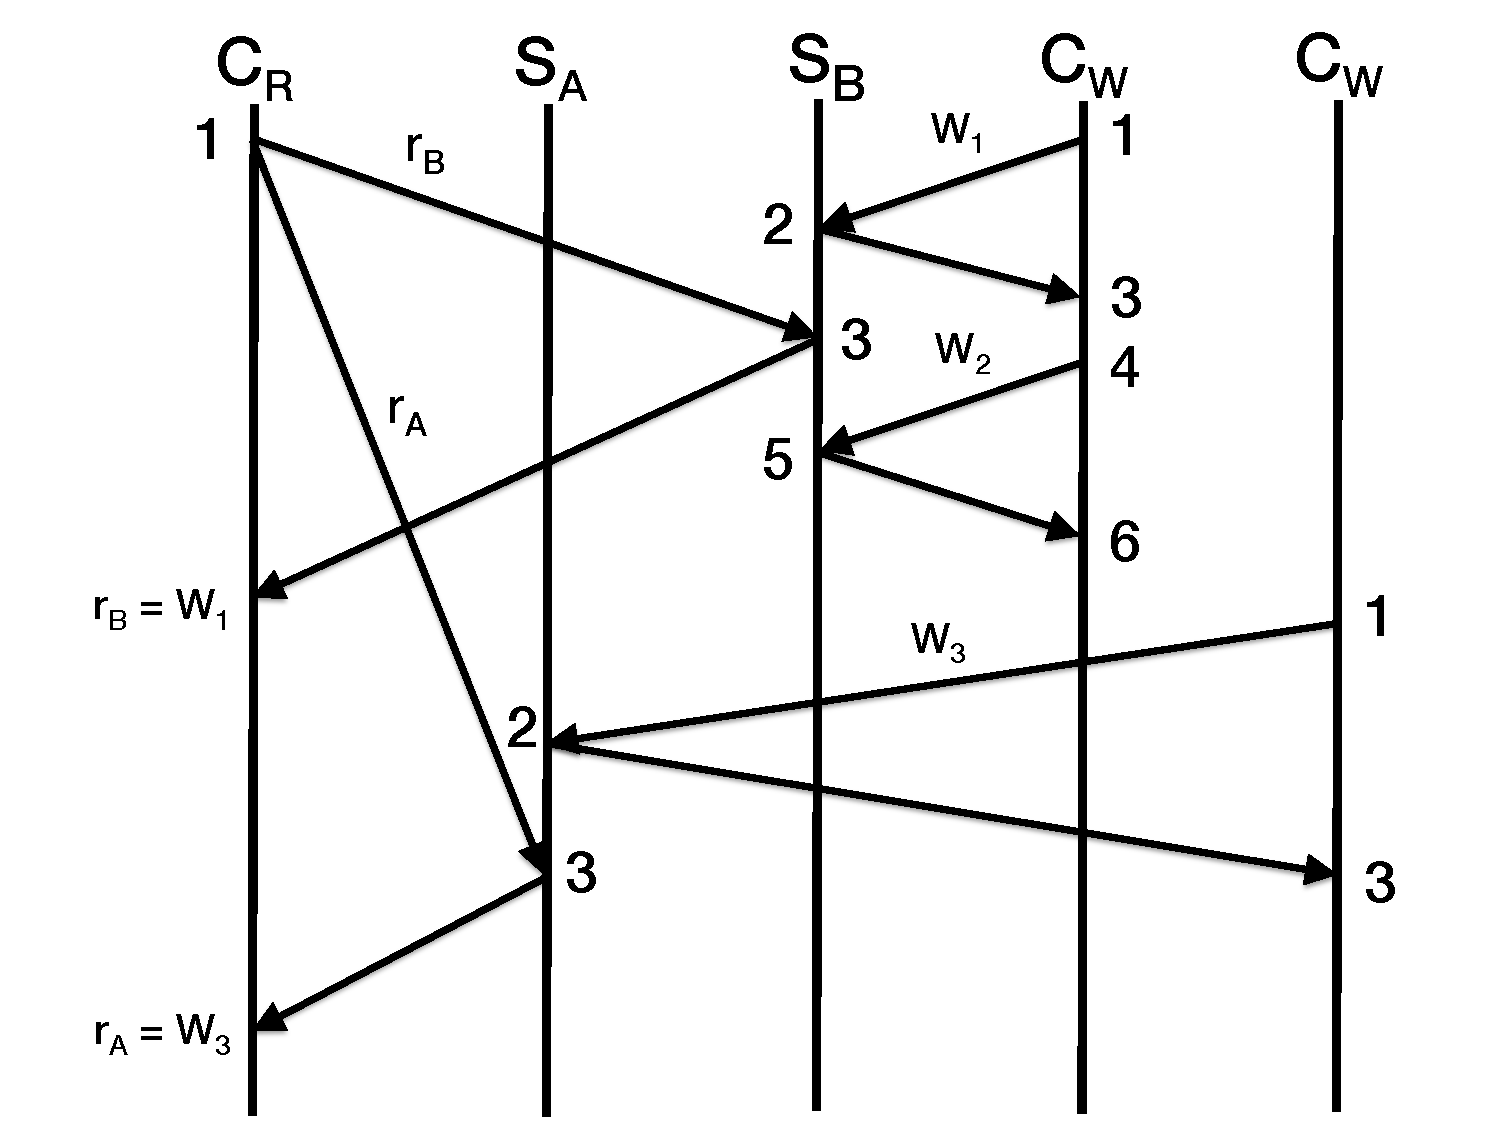
\includegraphics[width=1.0\columnwidth]{figures/eiger-example-2.pdf}
\caption{An example execution that shows Eiger's \textsc{READ} transaction algorithm is not strictly serializable. $w_1$, $w_2$, and $w_3$ are three writes, where $w_3$ is issued after $w_2$ finishes. $r_A$ and $r_B$ are read operations from the same \textsc{READ} transaction $R$, which is concurrent with all three writes. Each number is a value of the logical clock on the machine (process) as a result of message exchange.}
\label{fig:eigerrot}
\end{figure}


\section{Eiger's \rots{} are not Strictly Serializable}
\label{app:eiger_not_s}
%\label{sec:eigerrot}
Eiger~\cite{Lloyd:nsdi2013} targeted a geo-replicated setting, which provided causal consistency across wide areas with fast \textsc{READ} and \textsc{WRITE} transactions handled by each datacenter locally. While not focusing on making transactions strictly serializable, Eiger made a claim that its \textsc{READ} transactions within the local datacenter were strictly serializable. Thus, in SNOW, there was a claim that Eiger was the only system, which had bounded latency while providing the strongest guarantees, and the practical lower bound for property $O$ in existing SNW algorithms was three because Eiger's \textsc{READ} transactions required at most three rounds, i.e., the fewest in all examined existing work, were non-blocking, compatible with \textsc{WRITE} transactions, and were claimed to be strictly serializable. In this section, we correct this claim to be that there was no algorithm, which had bounded latency while providing the strongest guarantees by proving that Eiger's \textsc{READ} transactions are not strictly serializable. In Section~\ref{mwmr_snow_one_version, mwmr_snow_one_round, mwmr_snow_one_round}, we provide the first set of novel SNW algorithms that have bounded latency and prove they are correct.

The insight on why Eiger's \textsc{READ} transactions are not strictly serializable is that Eiger uses logical timestamps, i.e., Lamport clocks, to track the ordering of operations, and logical clocks are not able to identify the real-time ordering between operations that do not have causal relationship, i.e., operations from different processes. Strict serializability, however, requires the real-time ordering to be respected.

Figure~\ref{fig:eigerrot} is an example execution, which is allowed by Eiger but violates strict serializability. 
%$S_A$ and $S_B$ are two servers with initial values $old$. $w_1$ is a write operation that updates $S_A$ with value $new$. After $w_1$ finishes, $w_2$ is issued by another client different from the one who issued $w_1$, and updates $S_B$ with value $new$. Because $w_2$ starts after $w_1$ finishes, $w_2$ should be ordered after $w_1$ by the real-time ordering requirement of strict serializability, i.e., if a READ transaction sees $w_2$, it has to also observe the effect of $w_1$. Because $w_1$ and $w_2$ are from different clients and they do not have causal relationship, it is possible for $w_1$ to commit at the larger logical time than $w_2$, e.g., 10 as shown in Figure~\ref{fig:eigerrot}. $r_1$ and $r_2$ are from the same READ transaction and return $old$ from $S_A$ and $new$ from $S_B$. Because of the misordered logical timestamps, the result is acceptable to Eiger's READ transaction algorithm, but the result violates strict serializability because the READ transaction sees $w_2$ but not $w_1$.
Real time goes downwards in the diagram. Each number is a value of the Lamport clock on the machine (process) as a result of message exchange. Initially all processes have Lamport clock value $0$, and no messages happened before the execution in Figure~\ref{fig:eigerrot}. A \textsc{READ} transaction $R=\{r_A, r_B\}$ reads values on $S_A$ and $S_B$ respectively. Due to the asynchronous nature of the network, $r_B$ arrives on $S_B$ before $w_2$ and $r_A$ arrives after $w_3$. Following the \textsc{READ} transaction algorithm of Eiger, $r_A$ returns the value of $w_3$ and its valid logical duration, i.e., $[2,3]$. Similarly, $r_B$ returns the value of $w_1$ and its valid logical duration, i.e., $[2,3]$. Because the two logical durations overlap, Eiger claims the combined values of $r_A$ and $r_B$ are consistent and accept them. However, because $w_3$ starts after $w_2$ finishes, $w_3$ is in real time after $w_2$. By strict serializability, if a \textsc{READ} transaction sees the value of $w_3$, then it has to also observe the effect of $w_2$. Hence, $R$, which returns the values of $w_1$ and $w_3$, violates strict serializability.


\section{SNW + One version, MWMR setting}
\label{app:algrithmB}
\begin{algorithm*}[!ht]
  \begin{algorithmic}[2]
  
    \begin{multicols}{3}{\footnotesize
          \Statex  {\bf At writer $w$}
          \Part{{\it State Variables}}{   
          \Statex $z \in \mathbb N$, initially   $0$
            }\EndPart
%\Statex
    \Statex  {\bf  \Writetr{$(i_1, v_{i_1}), (i_2, v_{i_2}), \cdots, (i_p,  v_{i_p})$}   }
          \State $I\triangleq \{i_1, i_2, \cdots, i_p \}$
          %\State $S_{I}\triangleq \{s_{i_1}, s_{i_2}, \cdots, s_{i_p}\}$
        \Part{ \underline{\writeValue}} {
            %    \State $t_w \leftarrow (z +1,  \text{``id''})$; $z \leftarrow z +1 $
                \State ${\kappa} \leftarrow (z +1,  w)$; $z \leftarrow z +1 $
                 \For{$i \in I$} 
            \State Send \writeValueTag, $({\kappa}, v_{s_i})$ to server $s_i$
           \EndFor 
          \State  Await {\ackTag} from servers in  $S_I$.
        }\EndPart
        \Statex
            \Part{ \underline{\informSerializer}} {

                                      \For{$i \in [k]$} 
            \If{$i \in I$}
             \State $b_i \leftarrow 1$
             \Else
               \State $b_i \leftarrow 0$
            \EndIf
           \EndFor 
      %      \State $b_{i}\triangleq$   $v_i$ if  $i \in I$, otherwise $\bot$
                                            \State  Send  (\informSerializerTag, $({\kappa}, (b_{1}, \cdots, b_{k}))$) to   $s^*$

    %       \State $\tilde{o}_{i}\triangleq$   $o_i$ if  $i \in I$, otherwise $\bot$
                      %                      \State  Send  (\informSerializerTag, $(t_w, \tilde{o}_{1}, \cdots \tilde{o}_{k})$) to $s^*$
          %\State  Await {\ackTag} from reader $s^*$
          \State Receive ({\ackTag}, $t_w$) from  coordinator $s^*$
        }\EndPart
      }\end{multicols}
  % \end{algorithmic} 
  % \caption{Protocol for   ${\mathbf{write}(v^{(1)}, v^{(2)}, \cdots v^{(k)})_w}, w \in \mathcal{W}$ in  
  %   algorithm $C$.}
  % \label{fig:c-writer}
  %\end{algorithm}
  
  %\begin{algorithm}[!ht]
  % \begin{algorithmic}[1]  
\vspace{-1.5em}
 \\\hrulefill
\vspace{-1.5em}
      \begin{multicols}{3}{\footnotesize    
          \Statex  {\bf At reader $r$}
          \Statex  {\bf \Readtr{$ o_{i_1},  o_{i_2}, \cdots, o_{i_p}$}} 
          \State $I\triangleq \{i_1, i_2, \cdots, i_p \}$
          %\State $S_{I}\triangleq \{s_{i_1}, s_{i_2}, \cdots, s_{i_p}\}$
    % \Part{{\it State Variables}}{   
    %     \Statex $List$, an ordered from  $\mathcal{T} \times \{ o_1,\bot \} \times \cdots \times \{ o_k,\bot \} $,\\ ~~~~~initially  $List=[(t^0, o_1, \cdots o_k)]$
    %       }\EndPart
            \Part{ \underline{\getTagArray}} {
          \State  Send  (\getTagArrayTag) to server $s^*$
          \State  Receive response  $(t_r, ({\kappa}_1, {\kappa}_2, \cdots, {\kappa}_k))$ from  $s^*$
        }\EndPart 
            \Statex
          \Part{{\underline{{\readValue}}}}{ 
            % \State $\forall i, 1 \leq i \leq k$: $t_i^{max}  \leftarrow \max\{ t: (i, t) \in  Tags\}$
                     \For{$i \in  I$} 
            \State  Send (\readValueTag, ${\kappa}_i$) to $s_i$
           \EndFor 
            \State  Wait responses as $v_{i}$ for each $s_i\in S$
            \State Return  $(v_{i_1}, v_{i_2}, \cdots, v_{i_p})$
          }\EndPart
        }\end{multicols}
    % \end{algorithmic} 
    % \caption{The read protocol $\readd_r$,  for reader $r$ in  algorithm $C$.}
    % \label{fig:c-reader}
    %\end{algorithm}

%%%% ORIGINAL
%%%   \begin{algorithm}[!ht]
%%%     \begin{algorithmic}[1]
%%%       \begin{multicols}{2}{\footnotesize
    
  % \begin{algorithm*}[!ht]
  %   \begin{algorithmic}[2]
\vspace{-1.7em}
\\\hrulefill
\vspace{-1.5em}
      \begin{multicols}{3}{\footnotesize
          \Statex {\bf At server $s_i$ for any $i \in [k]$}
            \Part{{\it State Variables}}{ 
              \Statex $Vals\subset \mathcal{K} \times \mathcal{V}_i$, initially   $\{({\kappa}^0, v_i^0)\}$
              %\Statex $Vals_s \subset \mathcal{T} \times \mathcal{V}_s$, initially   $\{(t_0, v_s^0)\}$
              %             pair with a tag and a coded element, initially $(t_0, c_0)$.
              %\Statex $t_c$,  the commited tag, initially $t_0$
            %\Statex $List$, an ordered from  $\mathcal{T} \times \{ o_1,\bot \} \times \cdots \times \{ o_k,\bot \} $,\\ ~~~~~initially  $List=[(t^0, o_1, \cdots o_k)]$
\Statex $List$, a list  of  $\mathcal{K} \times \{ 0, 1 \}^k $, initially  $[({\kappa}^0, (1, \cdots 1))]$
            }\EndPart
            \Statex
            \Part {\underline{On recv (\writeValueTag, $({\kappa}, v)$) from  $w$}} {
                       \State   $Vals \gets   Vals \cup \{({\kappa}, v)\}$ 
              \State  Send {\ackTag} to writer $w$.
            }\EndPart
            \Statex
            \Part{{\underline{On recv  (\informSerializerTag, $({\kappa}, (b_{1}, \cdots b_{k}))$) from  $w$}}}{ 
                %   \State append $({\kappa}, (b_{1}, \cdots, b_{k}))$ to $List$
                                 \State $List  \leftarrow List \bigoplus~ ({\kappa}, (b_{1}, \cdots b_{k}))$ 
                   //$\bigoplus$ for append
          % \State Send {\ackTag} to  $w$
                  \State $tag \leftarrow |List|$ // $| \cdot |$ size of the list
            \State Send  ({\ackTag}, $tag$) to  $w$
          }\EndPart
                   
                        \Statex
            \Part{ \underline{On recv (\readValueTag, ${\kappa}$) from  $r$ }} {
              \State   Send $v_i$ s.t. $({\kappa}, v) \in Vals$  to  $r$
            }\EndPart 
          \Statex\Statex   /* used only by $s^*$ */
          
          \Part{ \underline{On recv {\getTagArrayTag} from  $r$ }} {
          \For{$i \in [k]$} 
                     \State $j^* \leftarrow \max \{ j : List[j].b_i =1 \}$
                     \State ${\kappa}_i = List[j^*].{\kappa}$
            %\State  send  ($t_1, t_2, \cdots, t_k$) to $s_i$
           \EndFor 
             \State  $t_r \triangleq \max_{1 \leq j \leq |List|} \{ j : List[j].b_i = 1 \wedge i \in I\}$ 
            \State  Send  ($t_r, ({\kappa}_1,{\kappa}_2, \cdots, {\kappa}_k)$) to $r$
            }\EndPart       
          }\end{multicols}
        \end{algorithmic} 
        \caption{The protocol for any  writer $w$, reader $r$ or server $s_i$ for  algorithm $B$.}\label{fig:algo_b}
      \end{algorithm*}
\begin{theorem} Any well-formed  and fair execution of algorithm $B$ is an implementation of  an object of type $\tilde{\mathcal{O}}_T$ in the MWMR setting, 
  with no client-to-client communication,  comprising of objects $o_1, o_2, \cdots o_k$ stored in servers $s_1, s_2, \cdots, s_k$, respectively; and it satisfies the SNoW  properties. %Algorithm $B$ also tolerates any client crash failures.
  \end{theorem}

\begin{proof} Below we show that algorithm $B$ satisfies the  SNoW properties. 
  
  \noindent{\emph{\underline{S property:}}} 
  Let $\beta$ be any fair execution  of  $B$ and 
 suppose all clients in $\beta$ behave in a well-formed
manner. Suppose $\beta$ contains no incomplete transactions and let  $\Pi$ be the set of transactions in $\beta$.  We define an irreflexive partial ordering ($\prec$) in $\Pi$ as follows:  if $\phi$ and $\pi$ are any two distinct transactions in $\Pi$ then we say 
  $\phi \prec \pi$ if either $(i)$ $tag(\phi) < tag(\pi)$ or $(ii)$ $tag(\phi) = tag(\pi)$ and $\phi$ is a \wot{} and $\pi$ is a \rot{}. Below we prove the $S$  property of $B$ by showing that  properties $P1$, $P2$, $P3$ and $P4$ of Lemma~\ref{lem:equivalence} hold for $\beta$. 
  
  \emph{P1:}   Clearly, from an inspection of the algorithm, 
   $tag(\pi) \in \mathbb{N}$. From inspection of the algorithm, each \wot{} increases the size of 
   $List$, and the value of the tags are  defined by the size of $List$. Therefore, there can be at 
   most a finite number of \wots{} such that can precede $\pi$ (w.r.t. $\prec$) in $\beta$.
    On the other hand, if $\pi$ is a \rot{} then since all \rot{}s are invoked by readers  in a well-formed manner,  and there are only finite number of readers 
  therefore, there cannot be an infinite number of \rot{}s such that they all 
  precede $\pi$ (w.r.t $\prec$).
  
   
    
  \emph{P2:}  Suppose $\phi$ and $ \pi$ are any two transactions in $\Pi$, such that, $\pi$ begins after $\phi$ completes. Then we show that we have  we cannot have $\pi \prec \phi$. Now, we consider four cases, depending on whether $\phi$ and $\pi$ are \rot{}s or \wots{}. 
  \begin{enumerate}
      \item [$(a)$] $\pi$ and $\phi$ are \wots{} invoked by writers $w_{\pi}$ and $w_{\phi}$, respectively. Since the size of $List$, in $s^*$ grows monotonically due to each \wot{}  hence  $w_{\pi}$ receives the  tag  from $s^*$ at least as high as $tag(\phi)$, so $\pi\not \prec \phi$.
        %
         \item [$(b)$] $\pi$ is a \rot{}, $\phi$ is a \wot{} invoked by reader  $r_{\pi}$ and writer $w_{\phi}$, respectively.  
          Since the size of $List$, in $s^*$,  grows monotonically,  because  $r_{\pi}$  invokes $\pi$ after $\phi$ completes hence $tag(\pi)$ is at least as high as $tag(\phi)$, so $\pi\not \prec \phi$.
        %
          \item[$(c)$]$\pi$ and $\phi$ are both \rot{}s  invoked by readers $r_{\pi}$ and $r_{\phi}$, respectively. 
             Since the size of $List$, in $s^*$, grows monotonically,  because   $w_{\pi}$ invokes $\pi$ after $\phi$ completes hence $tag(\pi)$ is at least as high as $tag(\phi)$, so $\pi\not \prec \phi$.
          %
           \item [$(d)$] $\pi$ is a \wot{}, $\phi$ is a \rot{}  invoked by writer $w_{\pi}$ and reader $r_{\phi}$, respectively.
           This case is simple because new values are added to $List$, in $s^*$,  only  by writers, and $tag(\pi)$  has to be larger than the tag of $\phi$ and hence   $\pi\not \prec \phi$. 
  \end{enumerate}
  
  
  \emph{P3:} This is from  the fact that any \wot{} always creates a unique tag and all tags are totally ordered since they all belong to $\mathbb{N}$
  
    \emph{P4:} Consider a \rot{} $\rho$ as $READ(o_{i_1}, o_{i_2}, \cdots, o_{i_q})$, in $\beta$. 
Let the returned value from $\rho$ be $\mathbf{v} \equiv $$(v_{i_1}, v_{i_2}, \cdots, v_{i_q})$ such that 
$1 \leq {i_1} <  {i_2} <  \cdots <  {i_q} \leq k$, where value  $v_{i_j}$ corresponds to $o_{i_j}$. 
  Suppose $tag(\rho) \in \mathbb{N}$ was created during some \wot{}, say $\phi$, i.e., $\phi$ is the \wot{} that 
  added the elements in index $(tag(\rho)-1)$ of $List$ at the coordinator $s^*$. Note that element in index $0$ contains the initial value.
  %because \rots{} do not generate new tags as they do not add any new item to the $Vals$ of any server.
   Now we consider two cases:
   
  \emph{Case $tag(\rho) = 1$.} We  know that it corresponds the initial default value $v_i^0$ at each sub-object $o_i$, and this equates to $\rho$ returning the default initial value for each sub-object.
   %
  % Therefore, $tag(\rho) = tag(\phi)$. 
   
   \emph{Case $tag(\rho) > 1$.} Then we argue that there exists no \wot{}, say $\pi$, that updated object $o_{i_j}$,   in $\beta$, such that,  $\pi \neq \phi$ and $\rho$ returns values written by $\pi$ and $\phi \prec \pi \prec \rho$. Suppose we assume the  contrary, which means $tag(\phi) < tag(\pi) < tag(\rho)$. The latter implies $tag(\phi)  = tag(\pi)$ which is not possible because 
  this contradicts the fact that for any two distinct \wots{} $tag(\phi) \neq tag(\pi)$  in any execution of   $B$.

  \noindent{\emph{\underline{N, o and W properties:}}}  Evident from an inspection of the algorithm.
  % for the  response steps  of the servers to the reader.
  \end{proof}



\section{SNW + One round, MWMR setting}
\label{app:algrithmC}
\begin{algorithm*}[!ht]
  \begin{algorithmic}[2]
  
    \begin{multicols}{3}{\footnotesize
          \Statex  {\bf At writer $w$}
          \Part{{\it State Variables}}{   
          \Statex $z \in \mathbb N$, initially   $0$
            }\EndPart
%\Statex
    \Statex  {\bf  \Writetr{$(i_1, v_{i_1}), (i_2, v_{i_2}), \cdots, (i_p,  v_{i_p})$}   }
          \State $I\triangleq \{i_1, i_2, \cdots, i_p \}$
          %\State $S_{I}\triangleq \{s_{i_1}, s_{i_2}, \cdots, s_{i_p}\}$
        \Part{ \underline{\writeValue}} {
            %    \State $t_w \leftarrow (z +1,  \text{``id''})$; $z \leftarrow z +1 $
                \State ${\kappa} \leftarrow (z +1,  w)$; $z \leftarrow z +1 $
                 \For{$i \in I$} 
            \State Send \writeValueTag, $({\kappa}, v_{s_i})$ to server $s_i$
           \EndFor 
          \State  Await {\ackTag} from servers in  $S_I$.
        }\EndPart
        \Statex
            \Part{ \underline{\informSerializer}} {

                                      \For{$i \in [k]$} 
            \If{$i \in I$}
             \State $b_i \leftarrow 1$
             \Else
               \State $b_i \leftarrow 0$
            \EndIf
           \EndFor 
      %      \State $b_{i}\triangleq$   $v_i$ if  $i \in I$, otherwise $\bot$
                                            \State  Send  (\informSerializerTag, $({\kappa}, (b_{1}, \cdots, b_{k}))$) to   $s^*$

    %       \State $\tilde{o}_{i}\triangleq$   $o_i$ if  $i \in I$, otherwise $\bot$
                      %                      \State  Send  (\informSerializerTag, $(t_w, \tilde{o}_{1}, \cdots \tilde{o}_{k})$) to $s^*$
          %\State  Await {\ackTag} from reader $s^*$
          \State Receive ({\ackTag}, $t_w$) from  coordinator $s^*$
        }\EndPart
      }\end{multicols}
  % \end{algorithmic} 
  % \caption{Protocol for   ${\mathbf{write}(v^{(1)}, v^{(2)}, \cdots v^{(k)})_w}, w \in \mathcal{W}$ in  
  %   algorithm $C$.}
  % \label{fig:c-writer}
  %\end{algorithm}
  
  %\begin{algorithm}[!ht]
  % \begin{algorithmic}[1]  
\vspace{-1.5em}
 \\\hrulefill
\vspace{-1.5em}
      \begin{multicols}{3}{\footnotesize    
          \Statex  {\bf At reader $r$}
          \Statex  {\bf \Readtr{$ o_{i_1},  o_{i_2}, \cdots, o_{i_p}$}} 
          \State $I\triangleq \{i_1, i_2, \cdots, i_p \}$
          %\State $S_{I}\triangleq \{s_{i_1}, s_{i_2}, \cdots, s_{i_p}\}$
    % \Part{{\it State Variables}}{   
    %     \Statex $List$, an ordered from  $\mathcal{T} \times \{ o_1,\bot \} \times \cdots \times \{ o_k,\bot \} $,\\ ~~~~~initially  $List=[(t^0, o_1, \cdots o_k)]$
    %       }\EndPart
            \Part{ \underline{\readValuesAndTags}} {
          \State  Send  (\getTagArrayTag) to server $s^*$
           \For{$i \in  I$} 
            \State  Send (\readValuesTag) to $s_i$
             \EndFor 
             
          \State  Receive response  $(t_r, ({\kappa}_1, {\kappa}_2, \cdots, {\kappa}_k))$ from  $s^*$
            % \State $\forall i, 1 \leq i \leq k$: $t_i^{max}  \leftarrow \max\{ t: (i, t) \in  Tags\}$
            \State  Wait responses as $Vals_{i}$ from each $s_i\in S_I$
            \State Return  $(v_{i_1}, v_{i_2}, \cdots, v_{i_p})$ s.t.  $({\kappa}_{j}, v_{j}) \in Vals_{j}$, $j\in I$
          }\EndPart
        }\end{multicols}
    % \end{algorithmic} 
    % \caption{The read protocol $\readd_r$,  for reader $r$ in  algorithm $C$.}
    % \label{fig:c-reader}
    %\end{algorithm}

%%%% ORIGINAL
%%%   \begin{algorithm}[!ht]
%%%     \begin{algorithmic}[1]
%%%       \begin{multicols}{2}{\footnotesize
    
  % \begin{algorithm*}[!ht]
  %   \begin{algorithmic}[2]
\vspace{-1.7em}
\\\hrulefill
\vspace{-1.5em}
      \begin{multicols}{3}{\footnotesize
          \Statex {\bf At server $s_i$ for any $i \in [k]$}
            \Part{{\it State Variables}}{ 
              \Statex $Vals\subset \mathcal{K} \times \mathcal{V}_i$, initially   $\{({\kappa}^0, v_i^0)\}$
              %\Statex $Vals_s \subset \mathcal{T} \times \mathcal{V}_s$, initially   $\{(t_0, v_s^0)\}$
              %             pair with a tag and a coded element, initially $(t_0, c_0)$.
              %\Statex $t_c$,  the commited tag, initially $t_0$
            %\Statex $List$, an ordered from  $\mathcal{T} \times \{ o_1,\bot \} \times \cdots \times \{ o_k,\bot \} $,\\ ~~~~~initially  $List=[(t^0, o_1, \cdots o_k)]$
\Statex $List$, a list  of  $\mathcal{K} \times \{ 0, 1 \}^k $, initially  $[({\kappa}^0, (1, \cdots 1))]$
            }\EndPart
            \Statex
            \Part {\underline{On recv (\writeValueTag, $({\kappa}, v)$) from  $w$}} {
                       \State   $Vals \gets   Vals \cup \{({\kappa}, v)\}$ 
              \State  Send {\ackTag} to writer $w$.
            }\EndPart
            \Statex
            \Part{{\underline{On recv  (\informSerializerTag, $({\kappa}, (b_{1}, \cdots b_{k}))$) from  $w$}}}{ 
                %   \State append $({\kappa}, (b_{1}, \cdots, b_{k}))$ to $List$
                                 \State $List  \leftarrow List \bigoplus~ ({\kappa}, (b_{1}, \cdots b_{k}))$ 
                   //$\bigoplus$ for append
          % \State Send {\ackTag} to  $w$
                  \State $tag \leftarrow |List|$ // $| \cdot |$ size of the list
            \State Send  ({\ackTag}, $tag$) to  $w$
          }\EndPart
                   
                        \Statex
            \Part{ \underline{On recv ({\readValuesTag}) from  $r$ }} {
              \State   Send $Vals$  to  $r$
            }\EndPart 
          \Statex\Statex   /* used only by $s^*$ */
          
          \Part{ \underline{On recv {\getTagArrayTag} from  $r$ }} {
          \For{$i \in [k]$} 
                     \State $j^* \leftarrow \max \{ j : List[j].b_i =1 \}$
                     \State ${\kappa}_i = List[j^*].{\kappa}$
            %\State  send  ($t_1, t_2, \cdots, t_k$) to $s_i$
           \EndFor 
             \State  $t_r \triangleq \max_{1 \leq j \leq |List|} \{ j : List[j].b_i = 1 \wedge i \in I\}$ 
            \State  Send  ($t_r, ({\kappa}_1,{\kappa}_2, \cdots, {\kappa}_k)$) to $r$
            }\EndPart       
          }\end{multicols}
        \end{algorithmic} 
        \caption{The protocol for any  writer $w$, reader $r$ or server $s_i$ for  algorithm $C$.}\label{fig:algo_c}
      \end{algorithm*}


      
\begin{theorem} Any well-formed  and fair execution of algorithm $B$ is an implementation of  an object of type $\tilde{\mathcal{O}}_T$ in the MWMR setting, 
  with no client-to-client communication,  comprising of objects $o_1, o_2, \cdots o_k$ stored in servers $s_1, s_2, \cdots, s_k$, respectively; and it satisfies the SNoW  properties. %Algorithm $B$ also tolerates any client crash failures.
  \end{theorem}

\begin{theorem} Any well-formed  and fair execution of algorithm $C$ is an implementation of  an object of type $\bar{\mathcal{O}}_T$ in the MWMR setting, 
  with no client-to-client communication,  comprising of objects $o_1, o_2, \cdots o_k$ stored in servers $s_1, s_2, \cdots, s_k$, respectively; and it satisfies the SN$\bar{o}$W  properties. %Algorithm $B$ also tolerates any client crash failures.
\end{theorem}
%In algorihtm C, when a server $s_i$ responds to a reader with the entire history of  update values $Vals_i$ for object $o_i$. This impractical behavior 
%can be circuvented by sending only the $W$ latest values of $o_i$ to a read request, where $W$ is the maximum number of possible {\sc write}s concurrent with any {\sc read}.

\begin{proof} Below we show that algorithm $C$ satisfies the  SN$\bar{o}$W properties. 
  
  \noindent{\emph{\underline{S property:}}} 
  Let $\beta$ be any fair execution  of  $B$ and 
 suppose all clients in $\beta$ behave in a well-formed
manner. Suppose $\beta$ contains no incomplete transactions and let  $\Pi$ be the set of transactions in $\beta$.  We define an irreflexive partial ordering ($\prec$) in $\Pi$ as follows:  if $\phi$ and $\pi$ are any two distinct transactions in $\Pi$ then we say 
  $\phi \prec \pi$ if either $(i)$ $tag(\phi) < tag(\pi)$ or $(ii)$ $tag(\phi) = tag(\pi)$ and $\phi$ is a {\sc write} and $\pi$ is a {\sc read}. Below we prove the $S$  property of $B$ by showing that  properties $P1$, $P2$, $P3$ and $P4$ of Lemma~\ref{lem:equivalence} hold for $\beta$.  The properties $P1$-$P4$ can be proved to hold in a manner very similar to algorithm $B$ (Section~\ref{mwmr_snow_one_version}). Therefore, we avoid repeating them. 

  \noindent{\emph{\underline{N, $\bar{o}$ and W properties:}}}  Evident from an inspection of the algorithm.
  % for the  response steps  of the servers to the reader.
  \end{proof}







\end{document}
